% Options for packages loaded elsewhere
\PassOptionsToPackage{unicode}{hyperref}
\PassOptionsToPackage{hyphens}{url}
\PassOptionsToPackage{dvipsnames,svgnames*,x11names*}{xcolor}
%
\documentclass[
  english,
  man, donotrepeattitle,floatsintext]{apa7}
\usepackage{lmodern}
\usepackage{amssymb,amsmath}
\usepackage{ifxetex,ifluatex}
\ifnum 0\ifxetex 1\fi\ifluatex 1\fi=0 % if pdftex
  \usepackage[T1]{fontenc}
  \usepackage[utf8]{inputenc}
  \usepackage{textcomp} % provide euro and other symbols
\else % if luatex or xetex
  \usepackage{unicode-math}
  \defaultfontfeatures{Scale=MatchLowercase}
  \defaultfontfeatures[\rmfamily]{Ligatures=TeX,Scale=1}
\fi
% Use upquote if available, for straight quotes in verbatim environments
\IfFileExists{upquote.sty}{\usepackage{upquote}}{}
\IfFileExists{microtype.sty}{% use microtype if available
  \usepackage[]{microtype}
  \UseMicrotypeSet[protrusion]{basicmath} % disable protrusion for tt fonts
}{}
\makeatletter
\@ifundefined{KOMAClassName}{% if non-KOMA class
  \IfFileExists{parskip.sty}{%
    \usepackage{parskip}
  }{% else
    \setlength{\parindent}{0pt}
    \setlength{\parskip}{6pt plus 2pt minus 1pt}}
}{% if KOMA class
  \KOMAoptions{parskip=half}}
\makeatother
\usepackage{xcolor}
\IfFileExists{xurl.sty}{\usepackage{xurl}}{} % add URL line breaks if available
\IfFileExists{bookmark.sty}{\usepackage{bookmark}}{\usepackage{hyperref}}
\hypersetup{
  pdftitle={Project Similarity Bias and Variance Neglect in Forecast Metric Evaluation},
  pdfauthor={Shir Dekel1, Micah Goldwater1, Dan Lovallo2, \& Bruce Burns1},
  pdflang={en-EN},
  pdfkeywords={structural alignment, similarity, variance neglect, Net Present Value, capital allocation},
  colorlinks=true,
  linkcolor=Blue,
  filecolor=Maroon,
  citecolor=Blue,
  urlcolor=Blue,
  pdfcreator={LaTeX via pandoc}}
\urlstyle{same} % disable monospaced font for URLs
\usepackage{graphicx}
\makeatletter
\def\maxwidth{\ifdim\Gin@nat@width>\linewidth\linewidth\else\Gin@nat@width\fi}
\def\maxheight{\ifdim\Gin@nat@height>\textheight\textheight\else\Gin@nat@height\fi}
\makeatother
% Scale images if necessary, so that they will not overflow the page
% margins by default, and it is still possible to overwrite the defaults
% using explicit options in \includegraphics[width, height, ...]{}
\setkeys{Gin}{width=\maxwidth,height=\maxheight,keepaspectratio}
% Set default figure placement to htbp
\makeatletter
\def\fps@figure{htbp}
\makeatother
\setlength{\emergencystretch}{3em} % prevent overfull lines
\providecommand{\tightlist}{%
  \setlength{\itemsep}{0pt}\setlength{\parskip}{0pt}}
\setcounter{secnumdepth}{-\maxdimen} % remove section numbering
% Make \paragraph and \subparagraph free-standing
\ifx\paragraph\undefined\else
  \let\oldparagraph\paragraph
  \renewcommand{\paragraph}[1]{\oldparagraph{#1}\mbox{}}
\fi
\ifx\subparagraph\undefined\else
  \let\oldsubparagraph\subparagraph
  \renewcommand{\subparagraph}[1]{\oldsubparagraph{#1}\mbox{}}
\fi
% Manuscript styling
\usepackage{upgreek}
\captionsetup{font=singlespacing,justification=justified}

% Table formatting
\usepackage{longtable}
\usepackage{lscape}
% \usepackage[counterclockwise]{rotating}   % Landscape page setup for large tables
\usepackage{multirow}		% Table styling
\usepackage{tabularx}		% Control Column width
\usepackage[flushleft]{threeparttable}	% Allows for three part tables with a specified notes section
\usepackage{threeparttablex}            % Lets threeparttable work with longtable

% Create new environments so endfloat can handle them
% \newenvironment{ltable}
%   {\begin{landscape}\begin{center}\begin{threeparttable}}
%   {\end{threeparttable}\end{center}\end{landscape}}
\newenvironment{lltable}{\begin{landscape}\begin{center}\begin{ThreePartTable}}{\end{ThreePartTable}\end{center}\end{landscape}}

% Enables adjusting longtable caption width to table width
% Solution found at http://golatex.de/longtable-mit-caption-so-breit-wie-die-tabelle-t15767.html
\makeatletter
\newcommand\LastLTentrywidth{1em}
\newlength\longtablewidth
\setlength{\longtablewidth}{1in}
\newcommand{\getlongtablewidth}{\begingroup \ifcsname LT@\roman{LT@tables}\endcsname \global\longtablewidth=0pt \renewcommand{\LT@entry}[2]{\global\advance\longtablewidth by ##2\relax\gdef\LastLTentrywidth{##2}}\@nameuse{LT@\roman{LT@tables}} \fi \endgroup}

% \setlength{\parindent}{0.5in}
% \setlength{\parskip}{0pt plus 0pt minus 0pt}

% Overwrite redefinition of paragraph and subparagraph by the default LaTeX template
% See https://github.com/crsh/papaja/issues/292
\makeatletter
\renewcommand{\paragraph}{\@startsection{paragraph}{4}{\parindent}%
  {0\baselineskip \@plus 0.2ex \@minus 0.2ex}%
  {-1em}%
  {\normalfont\normalsize\bfseries\itshape\typesectitle}}

\renewcommand{\subparagraph}[1]{\@startsection{subparagraph}{5}{1em}%
  {0\baselineskip \@plus 0.2ex \@minus 0.2ex}%
  {-\z@\relax}%
  {\normalfont\normalsize\itshape\hspace{\parindent}{#1}\textit{\addperi}}{\relax}}
\makeatother

% \usepackage{etoolbox}
\makeatletter
\patchcmd{\HyOrg@maketitle}
  {\section{\normalfont\normalsize\abstractname}}
  {\section*{\normalfont\normalsize\abstractname}}
  {}{\typeout{Failed to patch abstract.}}
\patchcmd{\HyOrg@maketitle}
  {\section{\protect\normalfont{\@title}}}
  {\section*{\protect\normalfont{\@title}}}
  {}{\typeout{Failed to patch title.}}
\makeatother
\shorttitle{Project Similarity Bias and Variance Neglect}
\keywords{structural alignment, similarity, variance neglect, Net Present Value, capital allocation\newline\indent Word count: 7040}
\usepackage{csquotes}
\raggedbottom
\renewcommand\author[1]{}
\renewcommand\affiliation[1]{}
\authorsnames[1, 1, 2, 1]{Shir Dekel, Micah Goldwater, Dan Lovallo, Bruce Burns}
\authorsaffiliations{{The University of Sydney, School of Psychology}, {The University of Sydney, Business School}}
\usepackage{pdflscape}
\newcommand{\blandscape}{\begin{landscape}}
\newcommand{\elandscape}{\end{landscape}}
\ifxetex
  % Load polyglossia as late as possible: uses bidi with RTL langages (e.g. Hebrew, Arabic)
  \usepackage{polyglossia}
  \setmainlanguage[]{english}
\else
  \usepackage[shorthands=off,main=english]{babel}
\fi
\ifluatex
  \usepackage{selnolig}  % disable illegal ligatures
\fi
\newlength{\cslhangindent}
\setlength{\cslhangindent}{1.5em}
\newenvironment{cslreferences}%
  {\setlength{\parindent}{0pt}%
  \everypar{\setlength{\hangindent}{\cslhangindent}}\ignorespaces}%
  {\par}

\title{Project Similarity Bias and Variance Neglect in Forecast Metric Evaluation}
\author{Shir Dekel\textsuperscript{1}, Micah Goldwater\textsuperscript{1}, Dan Lovallo\textsuperscript{2}, \& Bruce Burns\textsuperscript{1}}
\date{}


\authornote{

Shir Dekel \url{https://orcid.org/0000-0003-1773-2446}.

Portions of this work comprised Shir Dekel's doctoral dissertation.

Correspondence concerning this article should be addressed to Shir Dekel, Brennan MacCallum Building (A18) Camperdown, NSW 2006, Australia. E-mail: \href{mailto:shir.dekel@sydney.edu.au}{\nolinkurl{shir.dekel@sydney.edu.au}}

}

\affiliation{\vspace{0.5cm}\textsuperscript{1} The University of Sydney, School of Psychology\\\textsuperscript{2} The University of Sydney, Business School}

\abstract{
Business executives often have to allocate resources across very
dissimilar projects. They use financial measures, such as Net Present Value
(NPV) that simplify this difficult comparison because they aim to be equally
applicable to any kind of project, but these measures vary in their reliability.
Psychological research suggests that comparing alignable objects will be easier
than comparing non-alignable objects (Markman \& Gentner, \protect\hyperlink{ref-markman1993}{1993}; Markman \& Medin, \protect\hyperlink{ref-markman1995}{1995}). However, it
is unclear how alignment might moderate people's use of financial measure such
as NPV. We found that laypeople accommodate their use of a financial measure
(NPV) based on its reliability (as explicitly described in the introduction to
the task) when allocating resources to a set of alignable projects, but use it
regardless of reliability when allocating to a set of non-alignable projects.
However, when NPV reliability information was presented numerically using
ranges, participants' allocation did not depend on the ranges---participants
used NPV even when they had an opportunity to use the intrinsic features of the
project. Overall, however, participants relied on NPV more when projects were
low in alignment than when they were high in alignment. The result with
numerical reliability was replicated with Masters of Management students. Our
results demonstrate that considering dissimilar choices may hinder people's
ability to evaluate their importance, and that people might not be using useful
variance information in their decisions.
}



\usepackage{amsthm}
\newtheorem{theorem}{Theorem}
\newtheorem{lemma}{Lemma}
\newtheorem{corollary}{Corollary}
\newtheorem{proposition}{Proposition}
\newtheorem{conjecture}{Conjecture}
\theoremstyle{definition}
\newtheorem{definition}{Definition}
\theoremstyle{definition}
\newtheorem{example}{Example}
\theoremstyle{definition}
\newtheorem{exercise}{Exercise}
\theoremstyle{definition}
\newtheorem{hypothesis}{Hypothesis}
\theoremstyle{remark}
\newtheorem*{remark}{Remark}
\newtheorem*{solution}{Solution}
\begin{document}
\maketitle






















\hypertarget{project-similarity-bias-and-variance-neglect-in-forecast-metric-evaluation}{%
\section{Project Similarity Bias and Variance Neglect in Forecast Metric Evaluation}\label{project-similarity-bias-and-variance-neglect-in-forecast-metric-evaluation}}

One of the most important tasks faced by executives is the allocation of capital
within their companies. This requires the ranking of projects by importance and
predicted success, and allocating the limited capital accordingly (not unlike a
scientific funding agency). Ranking of projects necessitates comparing them
across a number of dimensions. For example, the executive of an oil company may
have received multiple oil exploration proposals. Determining what makes one oil
exploration project better than another is relatively simple. However, consider
a different scenario in which the executive must allocate capital between an oil
exploration project and an oil refinery project. The dimensions of oil refinery
projects that distinguish superior from inferior projects may be totally
different from those of oil exploration projects. Consider a funding agency
having to decide between two cognitive scientists or between a cognitive
scientist and a physicist in awarding a fellowship. What makes a physics
proposal better for the field of physics than a cognitive science proposal for
cognitive science?

Structure-mapping theory (Gentner, \protect\hyperlink{ref-gentner1983}{1983}; Gentner \& Markman, \protect\hyperlink{ref-gentner1997}{1997}) provides a model of
comparison that psychologically distinguishes these two kinds of allocation
tasks. This framework models comparison as a process of mapping and alignment of
the shared dimensions of two conceptual structures. This mapping process reveals
the shared dimensions of the two structures as well as the differences in those
shared dimensions (known as \emph{alignable differences}). For example, when
comparing two oil exploration projects, the process for measuring the quantity
of hydrocarbons in a prospective oil field may be identical, but the specific
quantities measured will differ. This is known as an alignable difference; that
is, the difference constrained within the same dimension. However, when
comparing an oil field and a refinery, there will be a significantly higher
number of \emph{non-alignable differences}, because the two domains do not share
component dimensions. That is, the dimensional structure of processes in the
exploration project will be substantially different from that of processes in
the refinery project, making it difficult to find meaningful alignments. With a
higher number of non-alignable differences, there are fewer opportunities to
make meaningful comparisons, leading to greater difficulty in predicting project
success and ranking projects. The present study experimentally examined project
comparisons and how such comparisons may affect capital allocation decisions.
The working hypothesis is that projects that have a higher number of alignable
differences will lead to more precise and informed project predictions and
rankings compared with projects with non-alignable differences.

However, what happens when a task demands that two domains be aligned but they
are too disparate to align? Experimentally, this territory is somewhat
uncharted. It is expected that, when required, people will grasp at any piece of
information available and attempt to abstract and infer that which is reasonable
to ease the alignment. This occurs frequently in business settings. Because
corporate enterprises continue to embrace diversification strategies in their
investments, they must constantly make capital allocation decisions involving
highly disparate domains. To overcome these difficult comparisons, executives
rely on various financial measures that, in theory, may be applied to any
project or business proposal. These financial measures work well to ease the
burden of difficult comparisons because they ignore the complexities of
individual projects and focus solely on financial information such as total cost
and projected profits. Therefore, projects that are difficult to compare may be
evaluated more easily by comparing individual numerical measures.

The most common financial measure that is used by executives in order to value
business project proposals is NPV (Graham et al., \protect\hyperlink{ref-graham2015}{2015}; Graham \& Harvey, \protect\hyperlink{ref-graham2001}{2001}; Remer et al., \protect\hyperlink{ref-remer1993}{1993}). NPV is
the difference between the forecasted revenue of a project and the initial
investment in its development (accounting for the time value of money), as shown
in Equation~\eqref{eq:npv}:

\begin{equation}
\text{NPV}=\sum_{t=0}^n \frac{R_t}{(1+i)^t}, \label{eq:npv}
\end{equation}

where \(t\) is the time of the cash flow, \(i\) is the discount rate, \(R_t\) is the
net cash flow, and \(n\) is the total number of periods. NPV is commonly used in
decisions about capital allocation and investment. The basic rule is that if a
project has a positive NPV, it is financially viable, and if it has a negative
NPV, it is not. However, the use of NPV has been criticised, by both academics
and practitioners (Fox, \protect\hyperlink{ref-fox2008}{2008}; Willigers et al., \protect\hyperlink{ref-willigers2017}{2017}). The main criticism is that there
can be underlying sources of variance in NPV that are not reflected in the final
measure, which is expressed as a single numerical value. For instance, NPV is
dependent on the projected cash inflows for each year of the project. However,
financial forecasting is frequently inaccurate and prone to optimism bias
(Lovallo \& Kahneman, \protect\hyperlink{ref-lovallo2003}{2003}; Puri \& Robinson, \protect\hyperlink{ref-puri2007}{2007}). Therefore, there is bound to be variation in the
reliability of NPV measures as a function of the forecasting error in the cash
flow calculations. Project duration and the discount rate are further sources of
variance that may be hidden by the single numerical value of NPV.

The secondary goal of this research is to investigate the extent to which people
are sensitive to variance information (from financial forecasting) when making
capital allocation decisions. This consideration is especially important in the
capital allocation situations illustrated above, when executives need to compare
projects with disparate domains and must, therefore, rely on NPV. This matters
because the NPV of different domains may have different underlying forecasting
error, potentially compromising the utility of using NPV as the basis of
comparison. Do executives sufficiently account for the inherent sources of
variance in the measure on which they rely so heavily? Research shows that
people are effective at extracting variance information when exposed to
numerical sequences (Rosenbaum et al., \protect\hyperlink{ref-rosenbaum2020}{2020}). However, they struggle to use variance
information when it is represented numerically (Batteux et al., \protect\hyperlink{ref-batteux2020}{2020}; Galesic \& Garcia-Retamero, \protect\hyperlink{ref-galesic2010}{2010}; Konold et al., \protect\hyperlink{ref-konold1993}{1993}; Vivalt \& Coville, \protect\hyperlink{ref-vivalt2021}{2021}).

\hypertarget{experiment-summary}{%
\subsection{Experiment Summary}\label{experiment-summary}}

Experiment~1 investigated the effect of project alignment on the decision-making
of naive participants asked to allocate capital to a set of fictional projects.
Naive participants were assumed to have no requisite knowledge about NPV
reliability; thus, NPV reliability level was manipulated by directly telling
participants whether or not the given NPV was reliable. For this experiment, it
was predicted that when projects are alignable, participants who are told NPV is
reliable would use it in their decision-making, while participants who are told
that NPV was unreliable would not use it in their decision-making. However, when
projects are not alignable, it was predicted that participants would use NPV,
regardless of the stated NPV reliability level.

Experiment~2 investigated the decision-making of management students in a
similar situation to Experiment~1. The main difference was that instead of
telling participants whether or not the NPV was reliable, the level of
\emph{numerical} NPV reliability---that is, the width of the numerical range around
the average NPV---was manipulated. Similar to Experiment~1, it was predicted
that participants would rely more on NPV in non-alignable projects than in
alignable projects. However, it was predicted that numerical reliability level
would have no effect because there is little evidence that people are sensitive
to variance information when it is shown numerically.

Experiment~3 also tested the effects of project alignment and reliability level
in a non-business population but manipulated both verbal and numerical
reliability to enable a direct comparison. The term \emph{reliability level} is used
to describe the manipulation of whether NPV was expressed as a reliable measure
or not, while \emph{reliability type} is used to describe the manipulation of whether
reliability was expressed verbally or numerically. Experiment~3 predicted a
reliability level effect for the verbal reliability condition but not the
numerical reliability condition. Further, this experiment used project
descriptions with clearer profitability indicators and added a larger selection
of business industries.

\hypertarget{alignment-2}{%
\section{Experiment~1}\label{alignment-2}}

Experiment~1 investigated the effects of project alignment and explicit NPV
reliability information on capital allocation decisions. The structural
alignment literature suggests that people place more weight on alignable
differences than they do on non-alignable differences. It was expected that
participants would rely more on NPV than on other product attributes in their
decision-making because NPV may be applied to every product. However, this
effect should vary with participants' perceived NPV reliability level. That is,
if other project dimensions are alignable, the use of NPV may depend on its
reliability. However, it was predicted that in projects with low alignment,
there will be a greater reliance on NPV as the sole alignable difference,
regardless of its stated reliability. These effects were measured by considering
the linear relationship between NPV and the money allocated to each project.
Critically, the NPV and intrinsic features of each project shown to participants
were inversely related. Therefore, a positive NPV trend will indicate a heavier
reliance on NPV, whereas a negative trend will indicate a heavier reliance on
the intrinsic project features. First, Experiment~1 tested the following omnibus
hypothesis:

\begin{hypothesis}[overall effect]
\protect\hypertarget{hyp:three-way-alignment-2}{}{\label{hyp:three-way-alignment-2} \iffalse (overall effect) \fi{} }The alignment \(\times\) reliability level \(\times\) NPV interaction is
significant.
\end{hypothesis}

Initially, specific effects were tested by excluding the no NPV condition (in
which participants were not given NPV information). Given the difficulty of
comparing dissimilar projects, participants were expected to rely more heavily
on NPV when project attributes are not alignable compared with when they are
alignable. Therefore, Experiment~1 tested the following hypothesis:

\begin{hypothesis}[alignment effect]
\protect\hypertarget{hyp:allocation-alignment-alignment-2}{}{\label{hyp:allocation-alignment-alignment-2} \iffalse (alignment effect) \fi{} }The linear NPV trend will be stronger for projects with low alignment than for
projects with high alignment.
\end{hypothesis}

Participants' budget allocations were expected to depend on the provided NPV
reliability information. However, this is more likely when there are multiple
aligned metrics from which to choose compared with when NPV only is alignable.
Therefore, Experiment~1 tested the following hypothesis:

\begin{hypothesis}[the NPV reliability level effect depends on alignment]
\protect\hypertarget{hyp:allocation-alignment-reliability-npv-alignment-2}{}{\label{hyp:allocation-alignment-reliability-npv-alignment-2} \iffalse (the NPV reliability level effect depends on alignment) \fi{} }The NPV \(\times\) reliability level interaction will be stronger in the high
alignment than in low alignment.
\end{hypothesis}

Specifically, when projects are similar, it is expected that participants will
rely more on NPV if they are told that NPV is reliable (leading to a positive
NPV trend) but more on the intrinsic features of projects if they are told that
NPV is unreliable (leading to a negative NPV trend). However, when projects are
dissimilar, it is expected that participants will rely solely on NPV, regardless
of what they are told about its reliability. Therefore, Experiment~1 tested the
following hypotheses:

\begin{hypothesis}[NPV reliability level in high alignment]
\protect\hypertarget{hyp:allocation-alignment-high-alignment-2}{}{\label{hyp:allocation-alignment-high-alignment-2} \iffalse (NPV reliability level in high alignment) \fi{} }When projects have high alignment, the NPV trend will be stronger when NPV
reliability is high compared with when NPV reliability is low.
\end{hypothesis}

\begin{hypothesis}[NPV reliability level in low alignment]
\protect\hypertarget{hyp:allocation-alignment-low-alignment-2}{}{\label{hyp:allocation-alignment-low-alignment-2} \iffalse (NPV reliability level in low alignment) \fi{} }When projects have low alignment, the NPV trend will not differ significantly
between the two reliability level conditions.
\end{hypothesis}

A no NPV condition was used to gain a better understanding of participants'
baseline response to materials when they had no information about NPV. The
extent of participants' reliance on NPV was determined by comparing this no NPV
condition to the conditions in which NPV was present. When projects are similar,
this condition was expected to be equivalent to the low NPV reliability
condition because in this condition participants should disregard NPV. When
projects are dissimilar, this condition was expected to show the average
participant value judgements of the project descriptions, because they only had
the intrinsic project features for their evaluations. This was expected to
result in a flat NPV trend. Therefore, Experiment~1 tested the following
hypotheses:

\begin{hypothesis}[effect of NPV information for projects with high alignment]
\protect\hypertarget{hyp:allocation-alignment-high-no-NPV-alignment-2}{}{\label{hyp:allocation-alignment-high-no-NPV-alignment-2} \iffalse (effect of NPV information for projects with high alignment) \fi{} }For projects with high alignment, the positive NPV trend will be stronger for
projects with high NPV reliability compared with projects with no NPV
information.
\end{hypothesis}

\begin{hypothesis}[effect of NPV information for projects with low alignment]
\protect\hypertarget{hyp:allocation-alignment-low-no-NPV-alignment-2}{}{\label{hyp:allocation-alignment-low-no-NPV-alignment-2} \iffalse (effect of NPV information for projects with low alignment) \fi{} }For projects with low alignment, the positive NPV trend will be stronger for
projects with both low and high NPV reliability compared with projects with no
NPV information.
\end{hypothesis}

\hypertarget{method}{%
\subsection{Method}\label{method}}

\hypertarget{participants}{%
\subsubsection{Participants}\label{participants}}

One hundred and eighteen participants (55 female) were recruited from the online recruitment platform Prolific. Participants were compensated at a rate of \pounds 5 an hour (Prolific is based in the UK). The average age was 29.42 years (\emph{SD} = 9.25, \emph{min.} = 18, \emph{max.} = 73).~Table~\ref{tab:condition-allocation-alignment-2}
shows the allocation of participants to the different conditions. NPV was varied
within subjects.

\begin{table}[tbp]

\begin{center}
\begin{threeparttable}

\caption{\label{tab:condition-allocation-alignment-2}Experiment 1 group allocation.}

\begin{tabular}{lll}
\toprule
Project alignment & \multicolumn{1}{c}{Reliability level of net present value (NPV)} & \multicolumn{1}{c}{N}\\
\midrule
High & High & 26\\
High & Low & 17\\
High & No NPV & 17\\
Low & High & 21\\
Low & Low & 16\\
Low & No NPV & 21\\
Total &  & 118\\
\bottomrule
\end{tabular}

\end{threeparttable}
\end{center}

\end{table}

\hypertarget{materials-alignment-2}{%
\subsubsection{Materials}\label{materials-alignment-2}}

\hypertarget{instructions-materials-alignment-2}{%
\paragraph{Instructions}\label{instructions-materials-alignment-2}}

Participants, who did not necessarily have business experience, were first shown
an instructions page with information about the task and NPV. These instructions
also informed participants about whether NPV as a financial measure was reliable
or unreliable for the specific project. Participants in the low NPV reliability
level conditions were told that NPV was an unreliable metric, while those in the
high NPV reliability level conditions were told that NPV was a reliable metric.
Instructions provided to participants in the no NPV condition did not include an
explanation of NPV or its reliability. Critically, participants were asked to
invest in products with a high objective value (because a higher-quality product
is not always better in the consumer goods market). Given that participants may
not use this instruction when directly viewing the projects, Experiment~3 used
projects whose attributes inherently expressed their quality.
Appendix~\ref{instructions-materials-alignment-2-appendix} shows the
instructions used in Experiment~1.

\hypertarget{projects-materials-alignment-2}{%
\paragraph{Project Display}\label{projects-materials-alignment-2}}

Participants were provided with a set of fictional business projects to which
they were asked to allocate capital. Alignment manipulation was reinforced
through visual presentation. Projects with high alignment were displayed in a
table listing their various attributes (see
Figure~\ref{fig:projects-alignment-high-materials-alignment-2}). In this group,
each project involved the same product type with consistent concrete attributes.
The table format was more appropriate for the high alignment condition because
all dimensions were shared. In contrast, projects with low alignment were
presented as paragraphs describing their relevant attributes (see
Figure~\ref{fig:projects-alignment-low-materials-alignment-2}). In this group,
each project was a different product with concrete attributes specific to that
product. In both alignment conditions, each project description included an NPV.
Critically, the values of the concrete attributes were always in conflict with
the NPV. For instance, Project 4 always had the lowest value for each concrete
attribute but always had the highest NPV. This meant that participants'
allocations could be used as a proxy for their degree of dependence on NPV.

Presentation style was potentially a confounding factor. This was addressed in
Experiment~3 by using the table format for both alignment conditions.



\begin{figure}
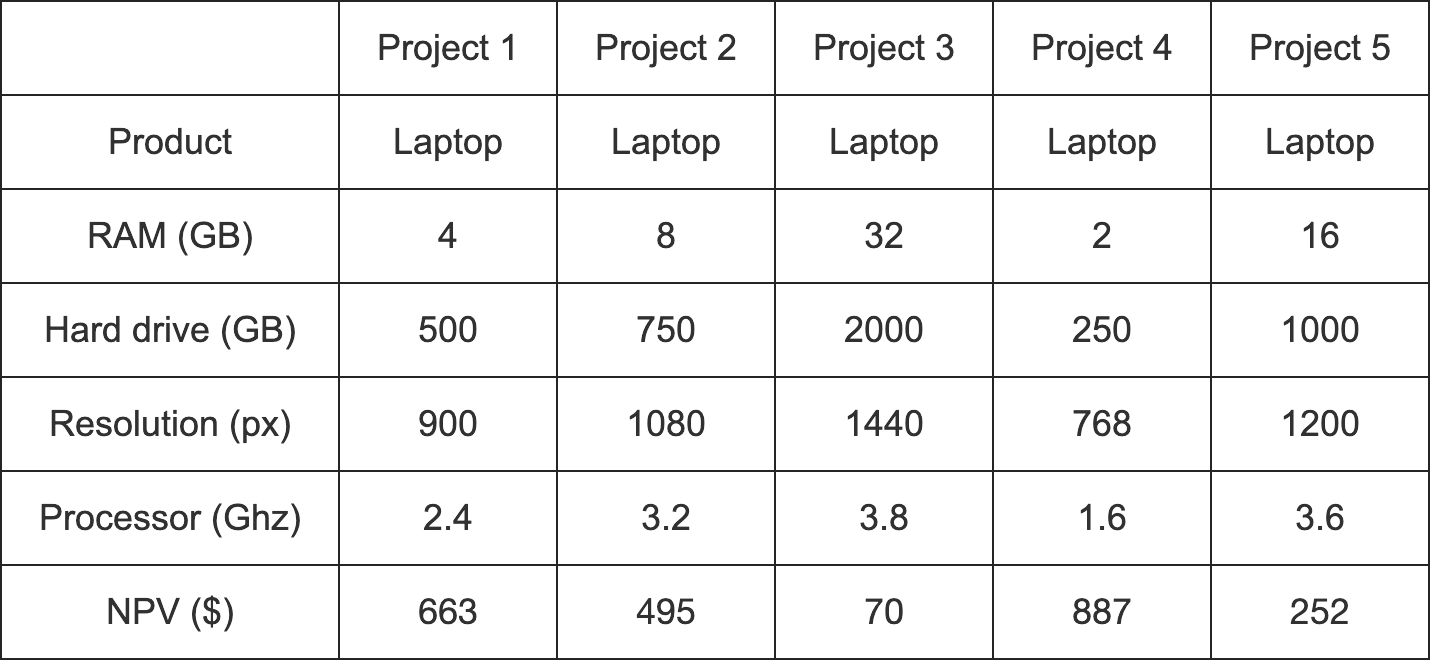
\includegraphics[width=1\linewidth]{project-similarity-bias-and-variance-neglect_files/figure-latex/projects-alignment-high-materials-alignment-2-1} \caption{An example of a high alignment display in Experiment~1.}\label{fig:projects-alignment-high-materials-alignment-2}
\end{figure}



\begin{figure}
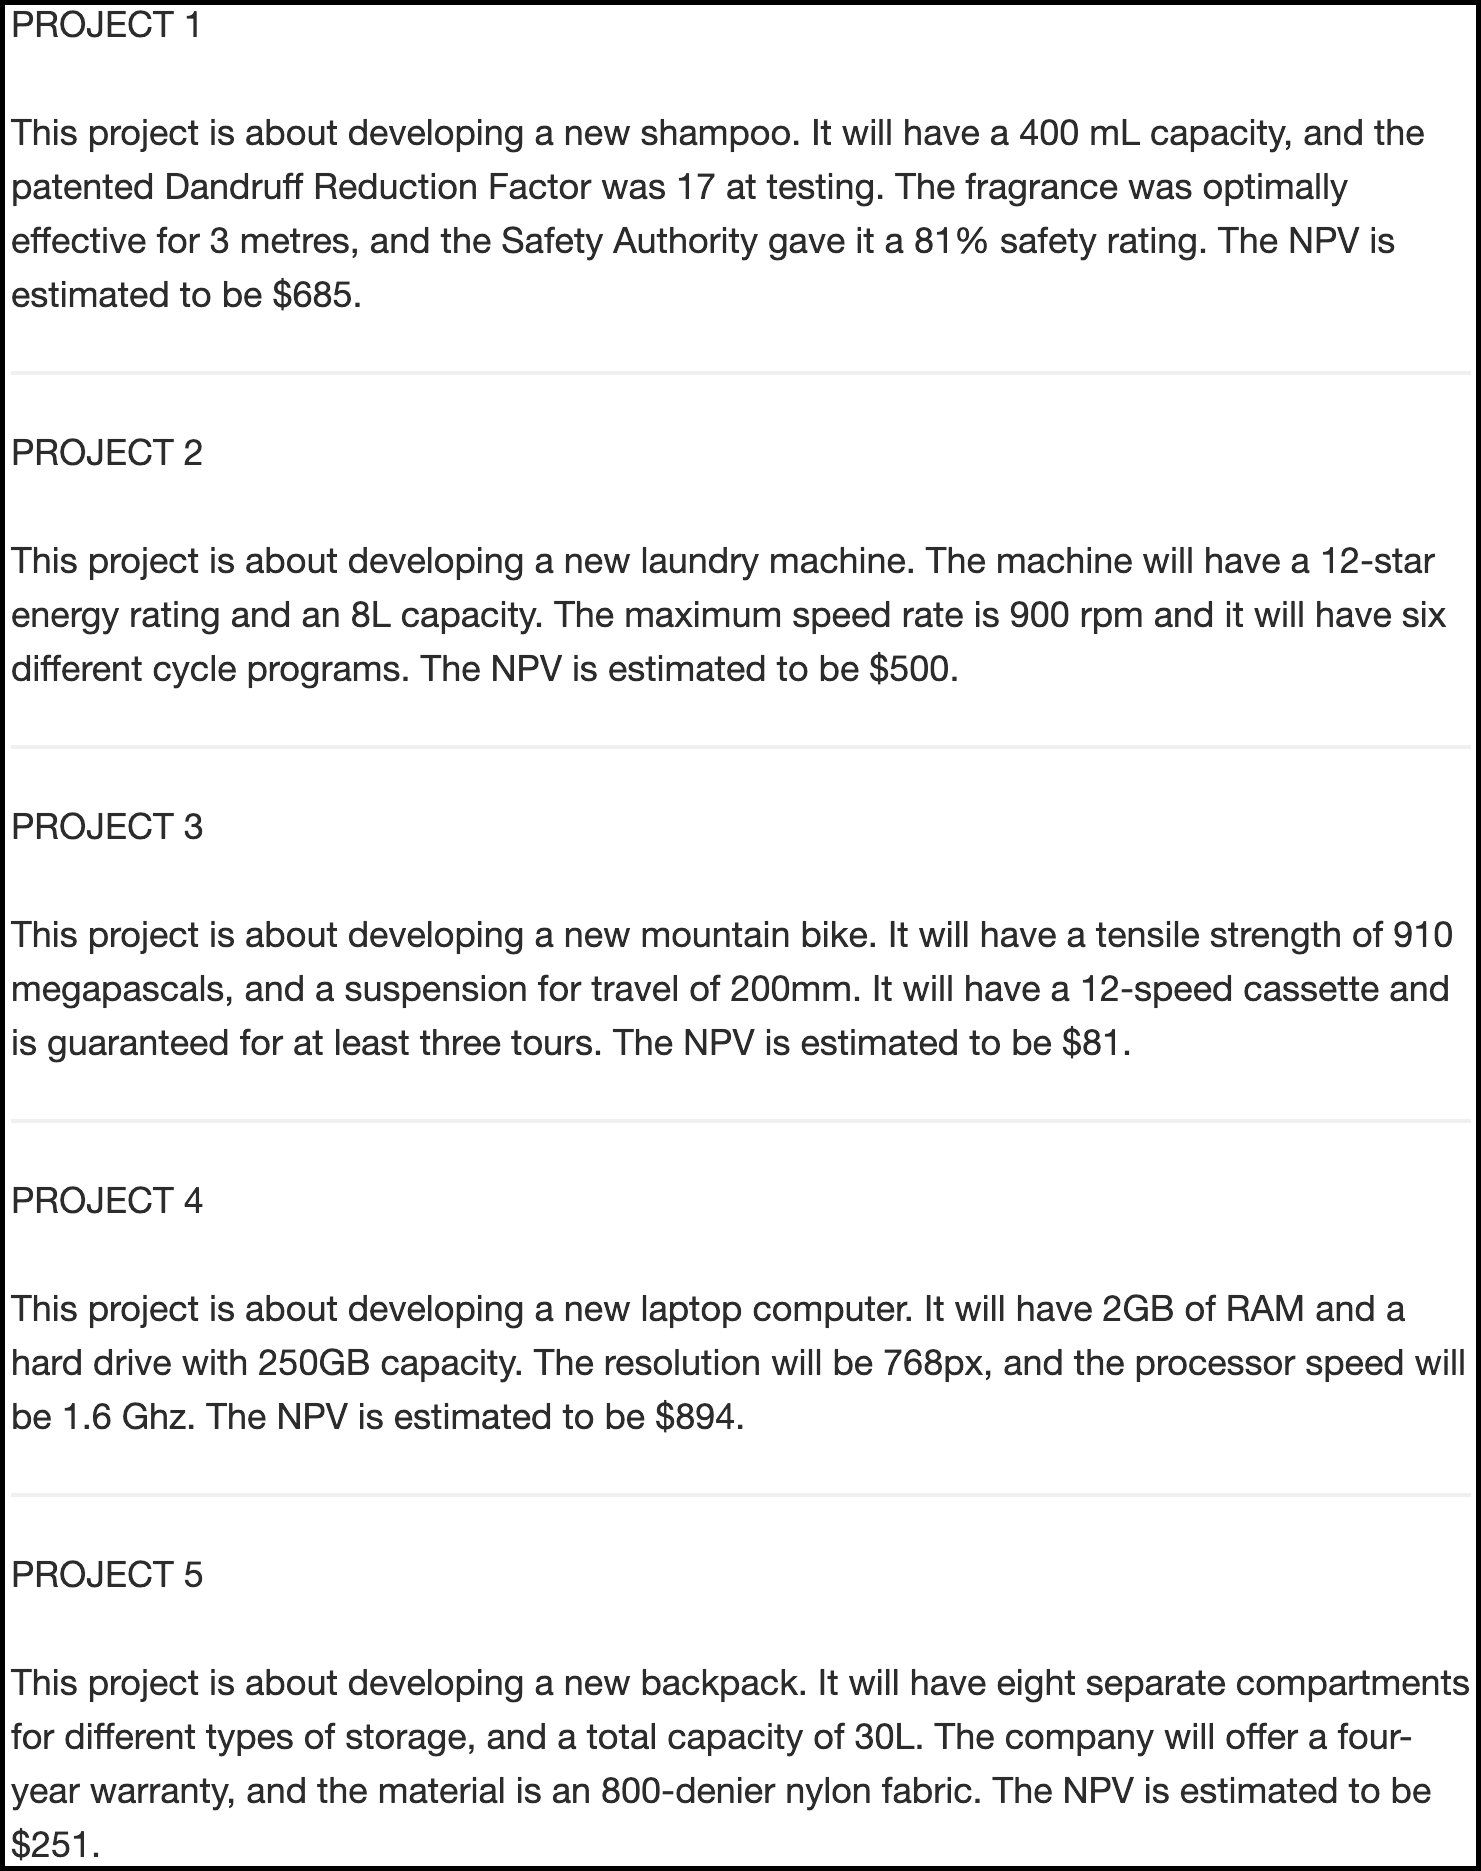
\includegraphics[width=1\linewidth]{project-similarity-bias-and-variance-neglect_files/figure-latex/projects-alignment-low-materials-alignment-2-1} \caption{An example of a low alignment display in Experiment~1.}\label{fig:projects-alignment-low-materials-alignment-2}
\end{figure}

\hypertarget{allocation}{%
\paragraph{Allocation}\label{allocation}}

Participants completed a capital allocation task (see
Figure~\ref{fig:allocation-alignment-2}) adapted from Bardolet et al. (\protect\hyperlink{ref-bardolet2011}{2011}) in which
they were asked to allocate a hypothetical yearly budget across the given five
projects.



\begin{figure}
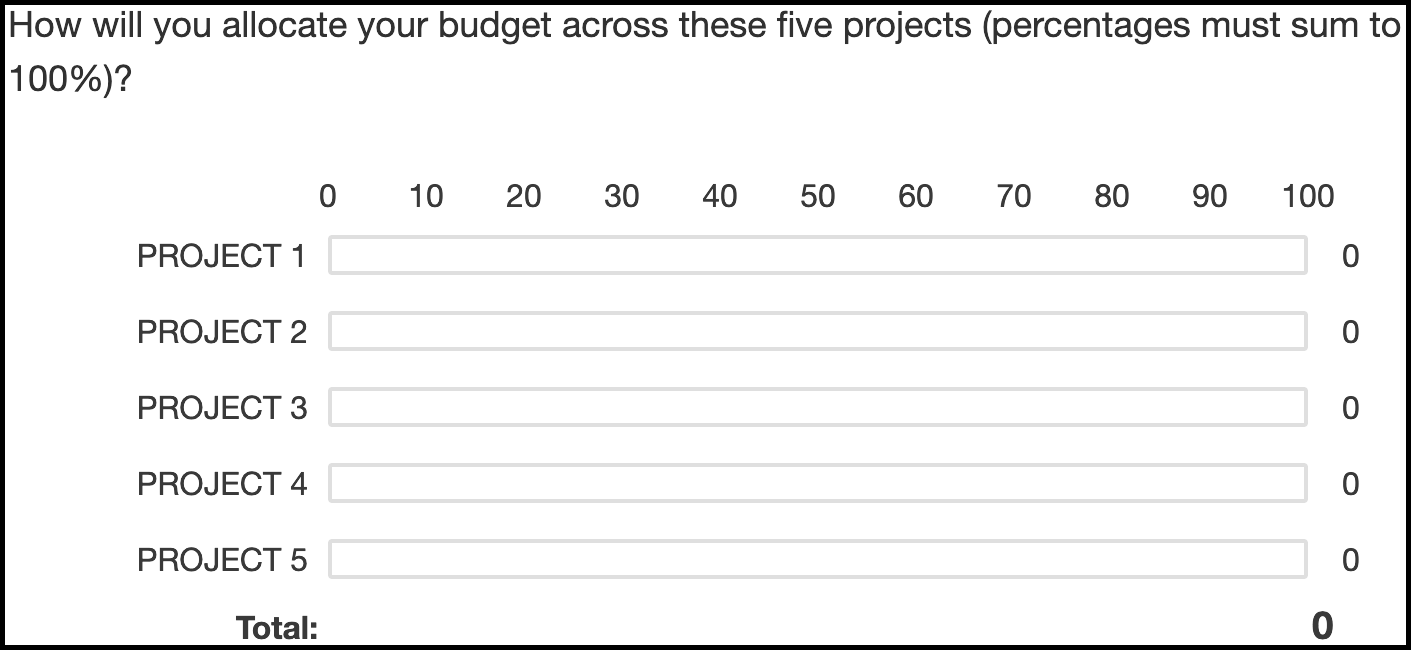
\includegraphics[width=1\linewidth]{project-similarity-bias-and-variance-neglect_files/figure-latex/allocation-alignment-2-1} \caption{The allocation task.}\label{fig:allocation-alignment-2}
\end{figure}

\hypertarget{additional-measures}{%
\paragraph{Additional Measures}\label{additional-measures}}

Other measures apart from allocation were included. The stimuli for and analyses
of these measures are reported in
Appendix~\ref{alignment-2-appendix}. Specifically,
participants were asked to forecast the future returns of the projects (see
Figure~\ref{fig:forecasting-materials-alignment-2}), rank the projects (see
Figure~\ref{fig:ranking-materials-alignment-2}), indicate their confidence in
their decisions (see Figure~\ref{fig:confidence-materials-alignment-2}), and
justify their decisions (see
Figure~\ref{fig:justification-materials-alignment-2}).

\hypertarget{procedure}{%
\subsubsection{Procedure}\label{procedure}}

After reading the relevant instruction page, participants allocated to the low
alignment conditions completed the forecasting task directly beneath each
project display. For the high alignment conditions, this was done directly
beneath all projects. Participants were then asked to rank the projects and
subsequently answer the allocation, confidence, and justification questions.

\hypertarget{results}{%
\subsection{Results}\label{results}}

A mixed factorial ANOVA was conducted to investigate the effects of project
alignment and NPV reliability level on participants' budget allocations. As
shown in Figure~\ref{fig:plot-alignment-2-allocation}, the alignment \(\times\)
NPV reliability level \(\times\) NPV interaction was significant,
\(F(6.57, 367.76) = 2.18\), \(p = .039\), \(\hat{\eta}^2_p = .038\). The
analyses excluding the no NPV condition showed the expected results. The NPV
trend averaged across both reliability level conditions was stronger for the low
alignment conditions than for the high alignment conditions,
\(\Delta M = 61.70\), 95\% CI \([33.02, 90.37]\), \(t(76) = 4.29\), \(p < .001\). This shows that people
relied more on NPV when projects were dissimilar than when they were similar.

Further, the NPV \(\times\) NPV reliability level interaction was stronger in the high
alignment conditions than in the low alignment conditions,
\(\Delta M = 67.81\), 95\% CI \([10.47, 125.16]\), \(t(76) = 2.36\), \(p = .021\). Specifically, in
the high alignment conditions, the NPV trend was stronger in the high NPV
reliability condition than in the low NPV reliability condition,
\(\Delta M = -63.47\), 95\% CI \([-100.00, -26.94]\), \(t(112) = -3.44\), \(p = .001\). In the low alignment
conditions, there was no significant difference between the two
reliability conditions, \(\Delta M = 4.35\), 95\% CI \([-34.52, 43.21]\), \(t(112) = 0.22\), \(p = .825\).
This shows that participants only used the NPV reliability information in their
allocation decisions when projects were similar, not when they were dissimilar.

The comparison with the no NPV condition revealed the expected pattern. For the
high alignment group, the linear NPV trend was significantly weaker in the no
NPV condition than in the high NPV reliability condition,
\(\Delta M = 75.70\), 95\% CI \([39.17, 112.24]\), \(t(112) = 4.11\), \(p < .001\), but not the low
NPV reliability condition, \(\Delta M = 12.24\), 95\% CI \([-27.94, 52.41]\), \(t(112) = 0.60\), \(p = .547\).
However, in the low alignment group, the linear NPV trend was significantly
weaker for the no NPV condition compared with both the low NPV reliability
condition, \(\Delta M = 64.63\), 95\% CI \([25.76, 103.50]\), \(t(112) = 3.29\), \(p = .001\),
and the high NPV reliability condition,
\(\Delta M = 60.29\), 95\% CI \([24.14, 96.43]\), \(t(112) = 3.30\), \(p = .001\).



\begin{figure}
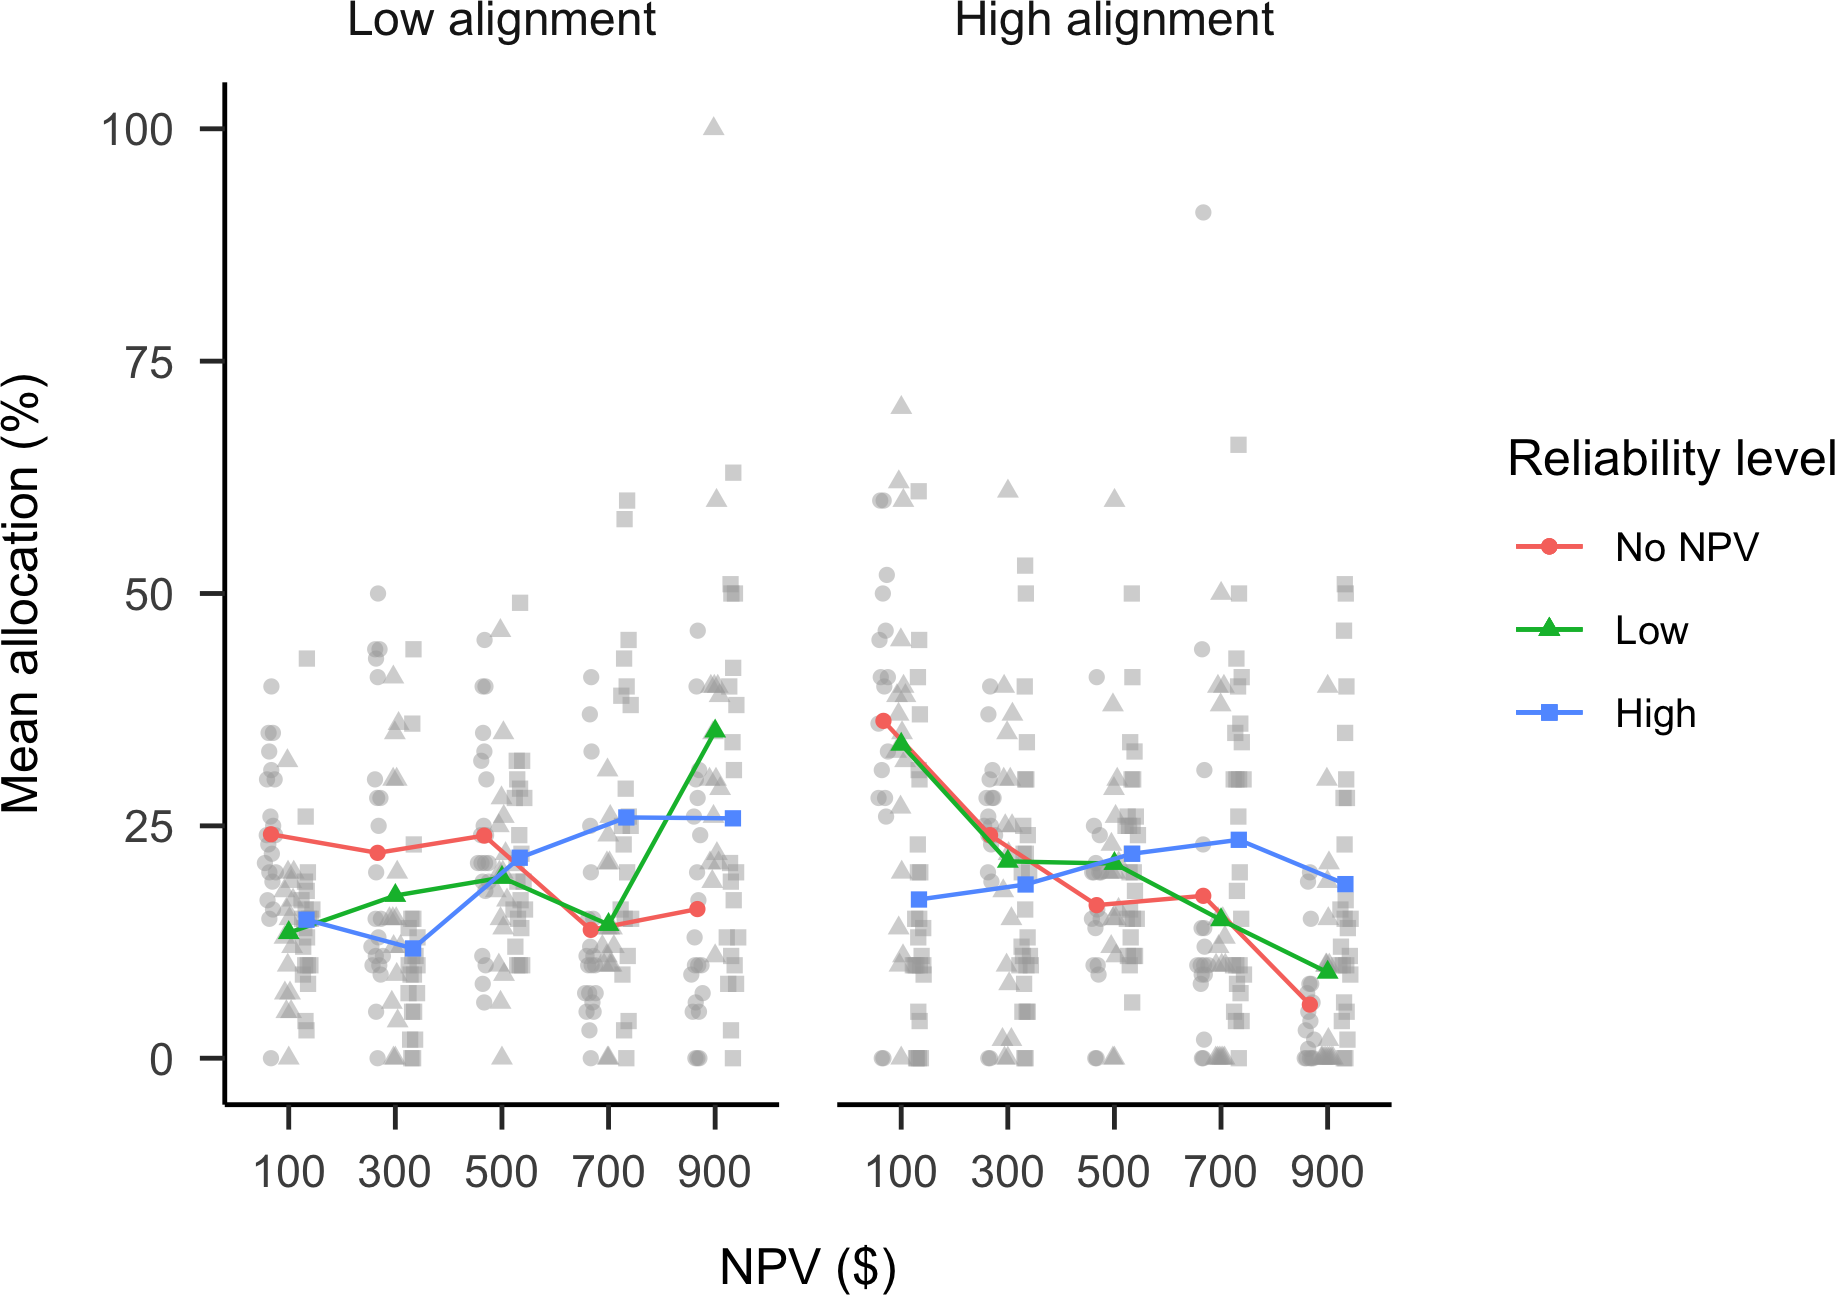
\includegraphics[width=1\linewidth]{project-similarity-bias-and-variance-neglect_files/figure-latex/plot-alignment-2-allocation-1} \caption{Mean allocation across NPV, by project alignment and reliability level conditions. In mixed factorial designs, error bars cannot be used to make inferences by ``eye'' across all conditions. Therefore, error bars are not included. Raw data are plotted in the background. When interpreting this figure, consider the linear trends in NPV.}\label{fig:plot-alignment-2-allocation}
\end{figure}

The mean ranking, confidence, and forecast data were all largely congruent with
the allocation findings (see Appendix~\ref{results-alignment-2-appendix}). The
results also show that the forecasts of those in the low alignment condition had
higher standard deviations than those in the high alignment condition (see
Appendix~\ref{forecast-sd-alignment-2}). However, this was not replicated in
follow-up experiments (Dekel, \protect\hyperlink{ref-dekel2021b}{2021}, Appendix B.5, \protect\hyperlink{ref-dekel2021b}{2021}, Appendix B.6).

\hypertarget{discussion}{%
\subsection{Discussion}\label{discussion}}

Experiment~1 found evidence for the effect of project alignment on laypeople's
decision-making in capital allocation scenarios. Specifically, when projects
were comparable, participants used NPV when they were told that it was reliable, but
did not when they were told that it was unreliable. However, they used NPV
regardless of its reliability when it was the only shared dimension across products.

Experiment~1 manipulated \emph{verbal} NPV reliability. That is, participants were
explicitly told whether NPV was considered to be a reliable metric or not.
However, in the real-world the reliability of a metric is more commonly
expressed in numerical form, such as a range around an estimate. Experiment~2
attempted to replicate the alignment effects, while manipulating the \emph{numerical}
NPV reliability associated with each project, rather than the verbal reliability
as used in Experiment~1. Further, people with sufficient experience with
financial theory and analysis may be able to successfully draw inferences from
such information. Therefore, Experiment~2 used a sample of students enrolled in
a Master of Management degree, instead of the laypeople used in Experiment~1.

\hypertarget{alignment-3}{%
\section{Experiment~2}\label{alignment-3}}

Experiment~2 investigated the effects of project alignment and
numerically-expressed NPV reliability information on capital allocation
decisions. In Experiment~1, the information about NPV reliability level was
communicated explicitly (e.g., ``NPV is unreliable''). However, in Experiment~2,
only the actual NPV information itself was communicated without the conclusion
about its reliability. Specifically, participants were given a range of
predicted values (akin to a confidence interval). Therefore, while Experiment~1
manipulated \emph{verbal} NPV reliability, Experiment~2 manipulated \emph{numerical} NPV
reliability. Further, Experiment~2 included participants with more business
experience. This experiment tested whether the previous findings of an alignment
effect would be replicated using participants with more business experience. The
experiment also tested whether this population is sensitive to variance in
forecasts.

Hypothesis~\ref{hyp:allocation-alignment-alignment-2} was again tested to
investigate the alignment effect in the new sample. However, the other
hypotheses tested in Experiment~1 were not retested because Experiment~2
manipulated numerical reliability and did not include a no NPV condition.
Research has shown that people are poor at reasoning with numerical variance
information (Batteux et al., \protect\hyperlink{ref-batteux2020}{2020}; Galesic \& Garcia-Retamero, \protect\hyperlink{ref-galesic2010}{2010}; Konold et al., \protect\hyperlink{ref-konold1993}{1993}; Vivalt \& Coville, \protect\hyperlink{ref-vivalt2021}{2021}). Therefore,
Experiment~2 tested the following hypothesis:

\begin{hypothesis}[no effect of numerical reliability]
\protect\hypertarget{hyp:allocation-npv-reliability-alignment-3}{}{\label{hyp:allocation-npv-reliability-alignment-3} \iffalse (no effect of numerical reliability) \fi{} }The NPV \(\times\) reliability level interaction is not significant in either
alignment condition.
\end{hypothesis}

Experiment~2 also investigated the ability to quickly change participants'
understanding, if they did not initially use numerical NPV reliability in their
allocations. Therefore, participants were presented with a short lecture on the
importance of paying attention to variance in financial decision-making.
However, this lecture was not sufficient to inform participants' use of
numerical reliability (see Appendix~\ref{alignment-3-appendix}). Further,
Experiment~2 investigated whether participants would be over-confident in their
understanding of NPV (as in Long et al., \protect\hyperlink{ref-long2018}{2018}). These results are also reported in
Appendix~\ref{alignment-3-appendix} because they are not highly relevant to
the present study.

\hypertarget{method-alignment-2}{%
\subsection{Method}\label{method-alignment-2}}

\hypertarget{participants-1}{%
\subsubsection{Participants}\label{participants-1}}

Fifty-four participants (28 female) were recruited from a Master of Management degree at an Australian university. Age information was not recorded.~Both the reliability level (low and high) and
project alignment (low and high) conditions were presented to subjects, and the
order of presentation was counterbalanced.

\hypertarget{materials}{%
\subsubsection{Materials}\label{materials}}

\hypertarget{instructions}{%
\paragraph{Instructions}\label{instructions}}

Participants were shown similar instructions to those used in Experiment~1.
However, they were given more NPV information (including discount rate and
initial investment). Appendix~\ref{instructions-materials-alignment-3-appendix}
shows the full instructions.

\hypertarget{npv-test}{%
\paragraph{NPV Test}\label{npv-test}}

Participants were asked to complete a short, simple test to check their
understanding of NPV (see Appendix~\ref{npv-test-materials-alignment-3}).

\hypertarget{project-display}{%
\paragraph{Project Display}\label{project-display}}

As shown in Figures~\ref{fig:projects-alignment-low-materials-alignment-3}
and~\ref{fig:projects-alignment-high-materials-alignment-3}, projects were
displayed as they were in Experiment~1. However, a second set of projects with
different product types and descriptions was added to enable within-subjects
manipulation. Along with the single numerical NPV, participants were provided
with the forecasted cash flow ranges used to calculate the NPV. In the low NPV
reliability condition, ranges were \(\pm85\)\% around the mean (e.g., \$150--\$1,850
if forecast mean was \$1,000); while in the high NPV reliability condition,
ranges were \(\pm5\)\% around the mean (e.g., \$950--\$1,050 if the forecast mean was
\$1,000). A wide range indicated that the measure had low reliability, while a
narrow range indicated that the measure had high reliability. Participants were
told to treat each set of projects independently.



\begin{figure}
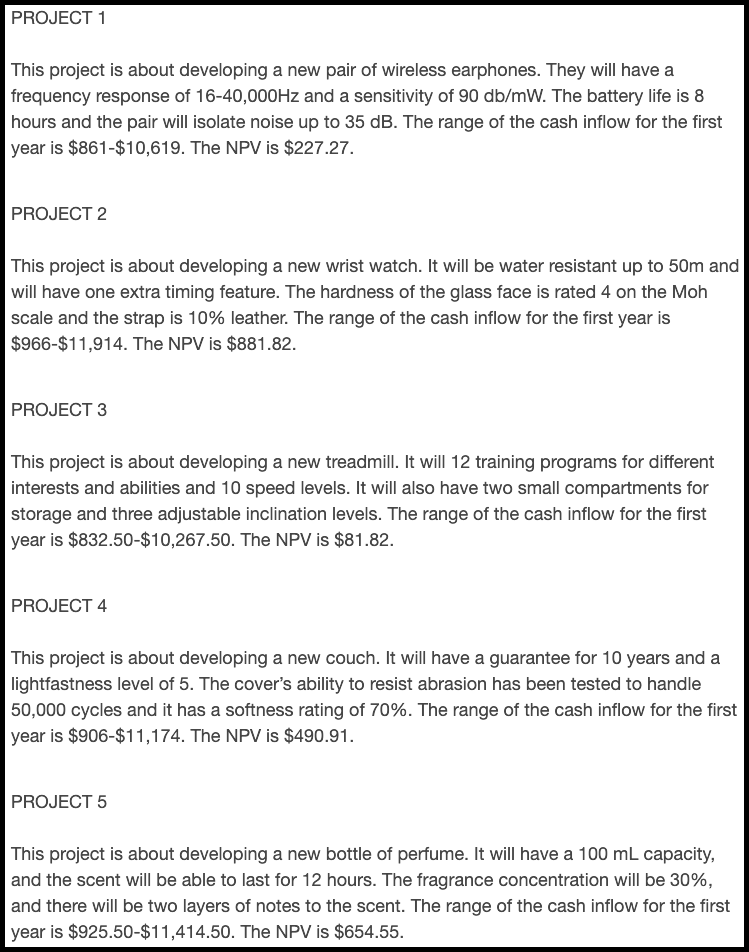
\includegraphics[width=1\linewidth]{project-similarity-bias-and-variance-neglect_files/figure-latex/projects-alignment-low-materials-alignment-3-1} \caption{An example of a low alignment, low reliability display in Experiment~2.}\label{fig:projects-alignment-low-materials-alignment-3}
\end{figure}



\begin{figure}
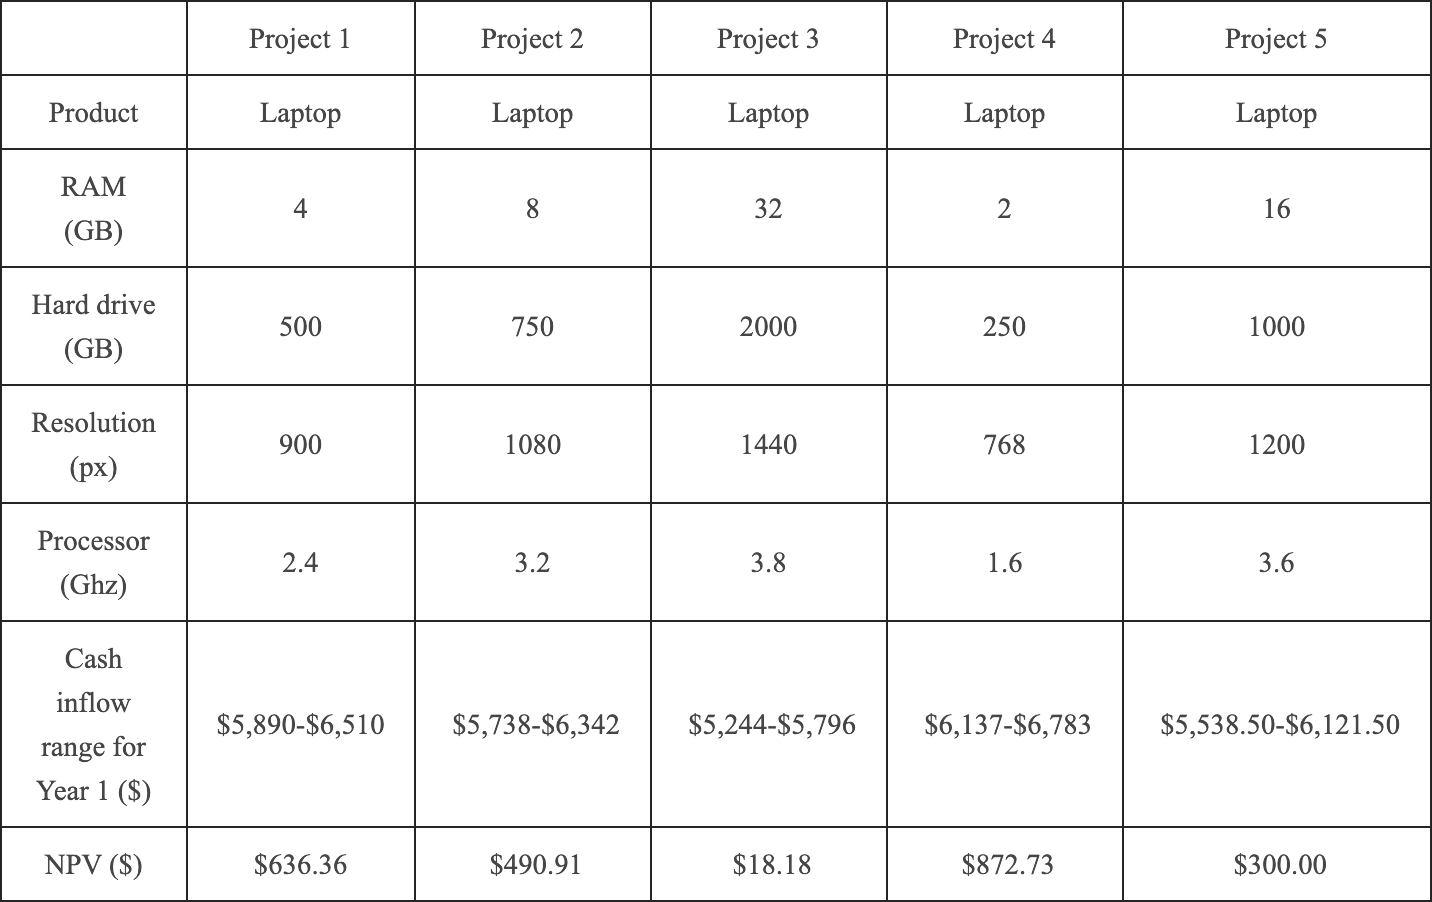
\includegraphics[width=1\linewidth]{project-similarity-bias-and-variance-neglect_files/figure-latex/projects-alignment-high-materials-alignment-3-1} \caption{An example of a high alignment, high reliability display in Experiment~2.}\label{fig:projects-alignment-high-materials-alignment-3}
\end{figure}

\hypertarget{npv-knowledge-ratings}{%
\paragraph{NPV Knowledge Ratings}\label{npv-knowledge-ratings}}

Participants were asked to rate their confidence in knowledge of NPV at multiple
points in the experiment. Appendix~\ref{npv-knowledge-materials-alignment-3}
shows an example of this display.

\hypertarget{variance-lecture}{%
\paragraph{Variance Lecture}\label{variance-lecture}}

Participants were given a short lecture on the importance of paying attention to
variance information in an attempt to increase their use of numerical
reliability information in their allocations (see
Appendix~\ref{variance-lecture-materials-alignment-3} for more details and the
lecture slides).

\hypertarget{procedure-alignment-3}{%
\subsubsection{Procedure}\label{procedure-alignment-3}}

Participants were provided with the instructions and an explanation of NPV
before completing a simple test to demonstrate their understanding of NPV. They
then completed four counterbalanced capital allocation trials (one for each
condition combination) before viewing a brief presentation on the importance of
paying attention to variance in financial decision-making. Participants then
repeated two of the trials that they had completed earlier. They were shown the
allocation values they had provided earlier and were given the opportunity to
change them. Participants rated their knowledge of NPV before and after
completing the NPV test and then rated it again after completing the four
project displays. They were then asked to rate their knowledge of NPV before and
after the variance presentation.

\hypertarget{results-alignment-2}{%
\subsection{Results}\label{results-alignment-2}}

A within-subjects factorial ANOVA was conducted to investigate the effects of
NPV, project alignment, and numerical NPV reliability on participants' project
allocations (see Figure~\ref{fig:plot-alignment-3-allocation}). The alignment
\(\times\) NPV reliability level \(\times\) NPV interaction was significant,
\(F(2.81, 148.75) = 3.95\), \(p = .011\), \(\hat{\eta}^2_p = .069\).
However, this appeared to be driven by the difference between alignment
conditions in the interaction between the quadratic NPV trend and NPV
reliability level,
\(\Delta M = -42.28\), \(95\%\ \mathrm{CI}_\mathrm{\scriptsize Sidak(5)}\) \([-76.96, -7.59]\), \(t(53) = -3.14\), \(p_\mathrm{\scriptsize Sidak(5)} = .011\), even after
applying a \v{S}idák correction. The same interaction but using a the linear NPV
trend was not significant,
\(\Delta M = -6.13\), \(95\%\ \mathrm{CI}_\mathrm{\scriptsize Sidak(5)}\) \([-31.50, 19.25]\), \(t(53) = -0.62\), \(p_\mathrm{\scriptsize Sidak(5)} = .954\). Further, the linear
NPV trend did not differ between the reliability level conditions in either the
low alignment condition, \(\Delta M = -3.19\), 95\% CI \([-18.77, 12.40]\), \(t(53) = -0.41\), \(p = .683\)
or the high alignment condition,
\(\Delta M = 2.94\), 95\% CI \([-12.63, 18.52]\), \(t(53) = 0.38\), \(p = .706\). However, averaged
across reliability level, the linear NPV trend was stronger in the low alignment
condition than in the high alignment condition,
\(\Delta M = 28.19\), 95\% CI \([5.57, 50.81]\), \(t(53) = 2.50\), \(p = .016\). This suggests that
participants relied more on NPV when projects were dissimilar compared with when
they were similar.



\begin{figure}
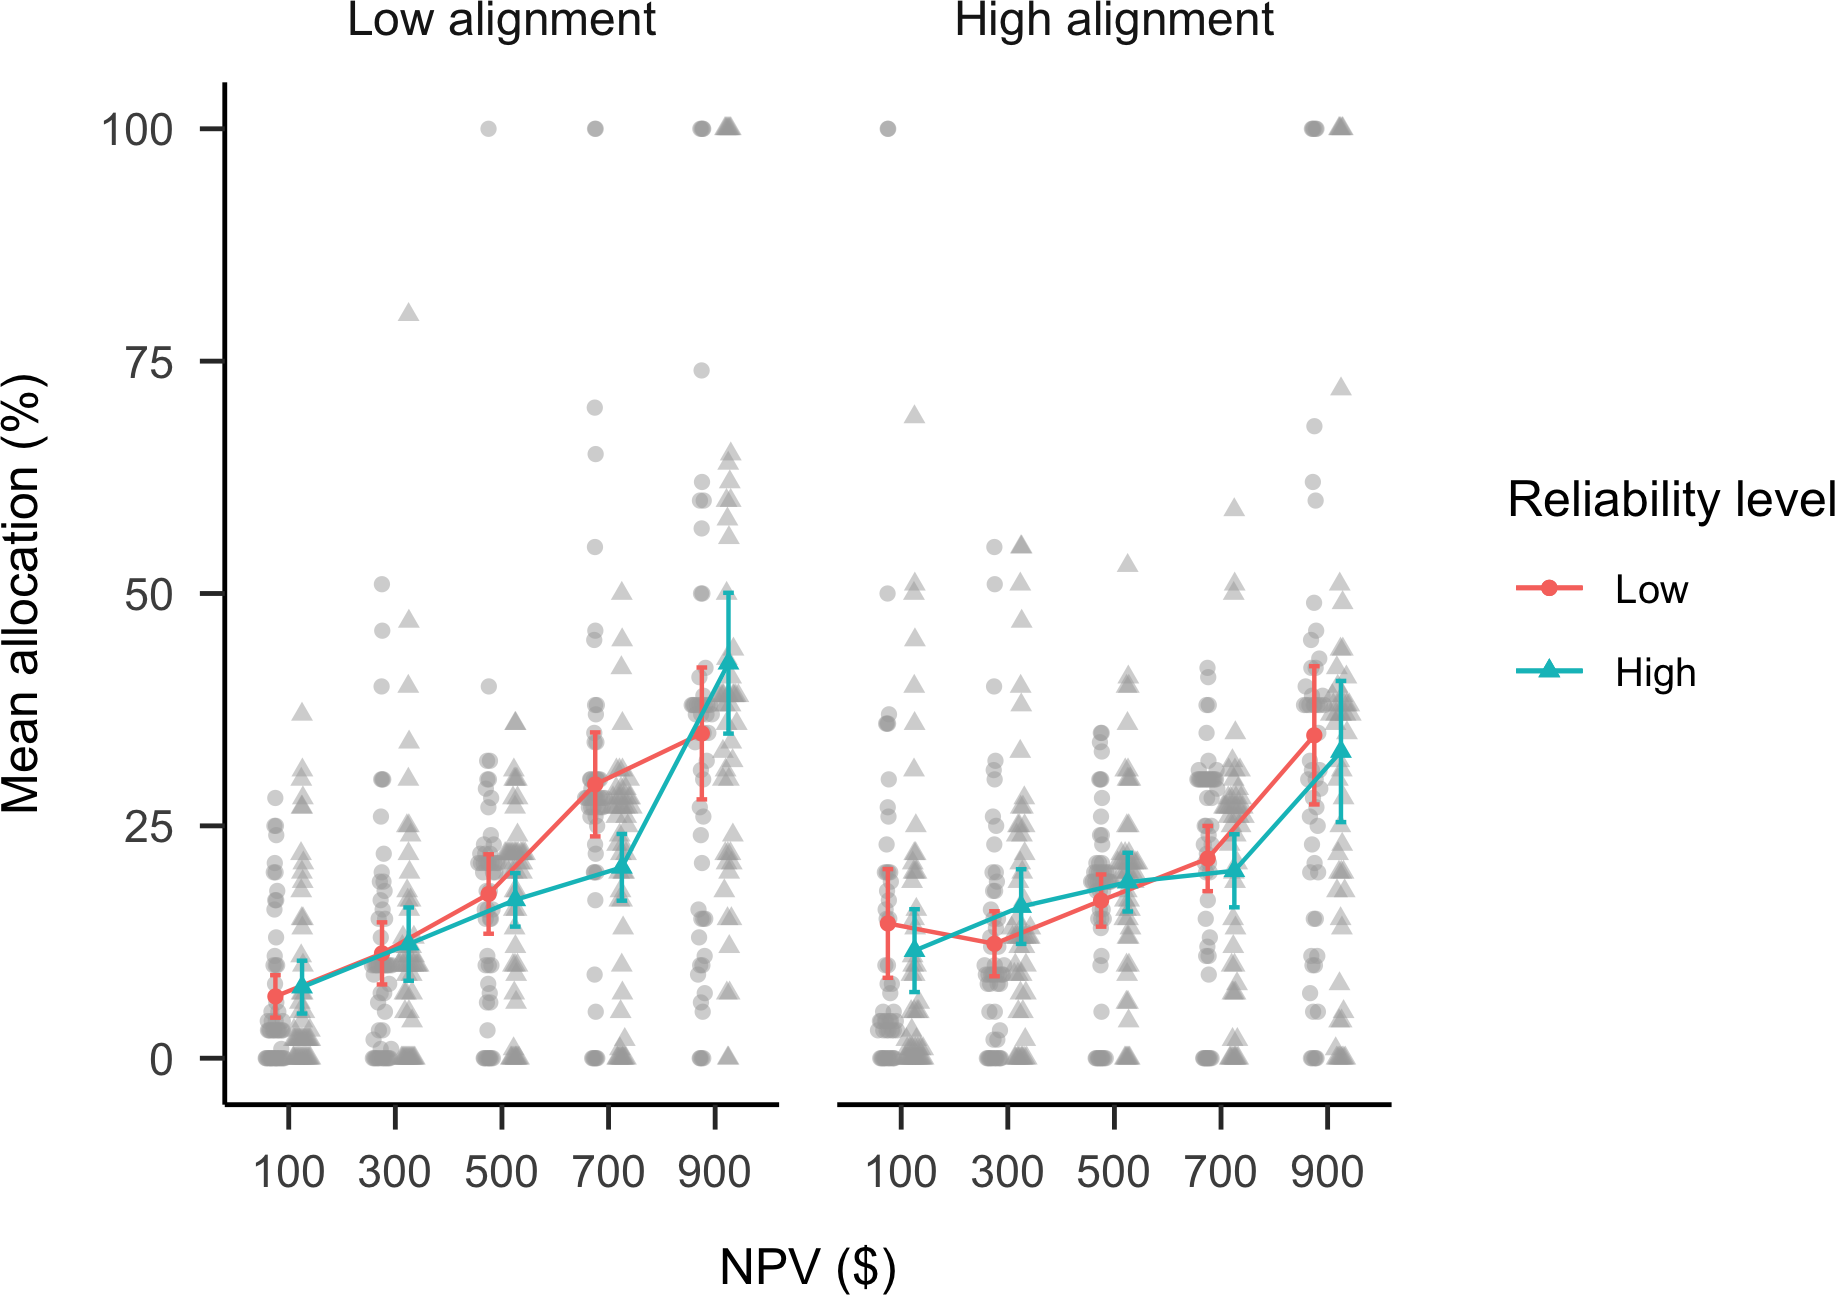
\includegraphics[width=1\linewidth]{project-similarity-bias-and-variance-neglect_files/figure-latex/plot-alignment-3-allocation-1} \caption{Mean allocation across NPV, by project alignment and reliability level conditions. Error bars represent 95\% confidence intervals, calculated from the within-subjects standard errors using the method from Cousineau and O'Brien (\protect\hyperlink{ref-cousineau2014}{2014}). Raw data are plotted in the background.}\label{fig:plot-alignment-3-allocation}
\end{figure}

The ranking data were congruent with these results, while the confidence data
were less so. Further, the findings on over-confidence from Long et al. (\protect\hyperlink{ref-long2018}{2018} Study~1)
were not replicated with NPV knowledge, and the variance lecture did not
facilitate participants' use of numerical reliability information. These
analyses are reported in Appendix~\ref{results-alignment-3-appendix}.

\hypertarget{discussion-1}{%
\subsection{Discussion}\label{discussion-1}}

Based on participants with real-world business experience, Experiment 2
replicated the alignment effect found in Experiment 1. That is, participants
relied more on NPV when faced with a set of dissimilar projects than when faced
with similar projects, supporting
Hypothesis~\ref{hyp:allocation-alignment-alignment-2}. Experiment~2 also found
evidence for Hypothesis~\ref{hyp:allocation-npv-reliability-alignment-3}, with
no significant differences between the numerical reliability conditions. While
Experiment~2 did not replicate the interaction found in Experiment~1, it should
be emphasised that these are two different effects. In Experiment~1,
participants were explicitly told whether the NPV measure was reliable, while in
Experiment~2, they were provided with variance information that merely implied
NPV reliability. Thus, the results of Experiment~2 show that business students
were affected by the comparability of projects but not by numerical NPV
reliability information. Specifically, participants appeared to focus only on
the NPV itself for a specific project, not on the underlying noisiness of the
measure.

The participants in Experiment~2 seemed to rely on NPV more than those in
Experiment~1. This was seen by the steeper linear trends in Experiment~2. This
discrepancy may be due to the difference in domain experience and exposure to
financial metrics in formal study. However, the extra explanation and testing of
NPV for the management students may have also increased its salience. In sum,
the Experiment~2 sample showed clearer trends of NPV reliance, but importantly
was still affected by similarity even when it was manipulated within-subjects.

Experiment~1 tested NPV reliability expressed verbally, while Experiment~2
tested NPV reliability expressed numerically. However, the difference in
findings was confounded by the different populations that were sampled. Further,
in both experiments, the business projects consisted of a limited number of
domains. It is unclear to what extent these specific domains influenced the
results. These projects were centred around consumer products, which were chosen
to be more easily accessible to participants without business experience.
However, the individual features of a project do not necessarily indicate its
profitability. For instance, a laptop with a low storage capacity may be more
profitable than one with a high storage capacity because of consumer goods
markets. Experiment~3 addressed these limitations.

Another limitation of Experiments~1 and~2 was the potential confounding effect
of presentation style. The two alignment conditions differed in the number of
alignable differences, but also in the way that the information was presented.
The information in the low alignment condition was presented as paragraphs,
while the information in the high alignment condition was presented as a table.
While it is likely that these data types would be presented in this way in the
business setting, it is important to rule out that this difference did not
unnecessarily increase task difficulty. Therefore, Experiment~3 attempted to
replicate this effect while controlling for presentation style

\hypertarget{alignment-8}{%
\section{Experiment~3}\label{alignment-8}}

Experiment~3 investigated the effects of project alignment, NPV, NPV reliability
type and NPV reliability level on participants' budget allocations. Experiment~1
manipulated NPV reliability level using verbal prompts. That is, participants
were explicitly told whether or not NPV was reliable for a certain project.
Experiment~2 investigated whether people were able to extract the same
reliability information using numerical prompts. That is, participants were
provided with NPVs with either wide or narrow ranges, indicating either low or
high reliability, respectively. Moreover, given that laypeople were sampled for
Experiment~1, and Master of Management students were sampled for Experiment~2,
it was not possible to compare the two reliability types (verbal and numerical)
without ruling out the potential confounding effect of population type. Thus,
similar to Experiments~1 and~2, Experiment~3 manipulated project alignment, NPV
and NPV reliability level but also added reliability type. Further, presentation
style was a possible confounding factor in the previous experiments. That is,
projects in the high alignment condition were always displayed in a table, while
projects in the low alignment condition were always displayed as paragraphs.
This possible confounder was excluded in Experiment~3 by using the same
presentation style for both alignment conditions.

In Experiment~3, the expected results for the verbal reliability condition
replicated those of Experiment~1. The numerical reliability condition may
replicate the findings of Experiment~2. However, a pilot experiment
(Dekel, \protect\hyperlink{ref-dekel2021b}{2021}, Appendix B.8) found no significant differences between numerical
reliability conditions. Appendix~\ref{alignment-8-appendix} shows a simulation
of the hypothesised effects, with the numerical reliability effects based on the
findings of the pilot experiment. Therefore, Experiment~3 retested
Hypotheses~\ref{hyp:three-way-alignment-2},~\ref{hyp:allocation-alignment-alignment-2},~\ref{hyp:allocation-alignment-reliability-npv-alignment-2},~\ref{hyp:allocation-alignment-high-alignment-2},
and~\ref{hyp:allocation-alignment-low-alignment-2} for the verbal reliability
condition, but was agnostic between whether the numerical reliability condition
will look more like the pattern found in the pilot experiment or the pattern
found in Experiment~2.

\hypertarget{method-1}{%
\subsection{Method}\label{method-1}}

\hypertarget{participants-2}{%
\subsubsection{Participants}\label{participants-2}}

Four hundred and forty-eight participants (176 female) were recruited from the online recruitment platform Prolific. Participants were compensated at a rate of \pounds 5 an hour (Prolific is based in the UK). The average age was 41.65 years (\emph{SD} = 10.3, \emph{min.} = 29, \emph{max.} = 78). Participants reported an average of 6.94 years (\emph{SD} = 8.23, \emph{min.} = 0, \emph{max.} = 43) working in a business setting, and an average of 3.73 years (\emph{SD} = 6.27, \emph{min.} = 0, \emph{max.} = 45) of business education. The mean completion time of the task was 11.35 min (\emph{SD} = 10.79, \emph{min.} = 1.92, \emph{max.} = 183.7).~Table~\ref{tab:condition-allocation-alignment-8}
shows the allocation of participants to the different conditions. The two
reliability level conditions (low and high) were presented within subjects and
the order of their presentation was randomised. Similar to the previous
experiments, NPV varied within subjects. Therefore, each participant saw two
separate project displays. Appendix~\ref{power-analysis-alignment-8} describes
the power analysis conducted to arrive at the sample size.

\begin{table}[tbp]

\begin{center}
\begin{threeparttable}

\caption{\label{tab:condition-allocation-alignment-8}Experiment 3 group allocation.}

\begin{tabular}{lll}
\toprule
Project alignment & \multicolumn{1}{c}{Reliability type} & \multicolumn{1}{c}{N}\\
\midrule
High & Explicit & 112\\
High & Implicit & 112\\
Low & Explicit & 112\\
Low & Implicit & 112\\
Total &  & 448\\
\bottomrule
\end{tabular}

\end{threeparttable}
\end{center}

\end{table}

\hypertarget{materials-1}{%
\subsubsection{Materials}\label{materials-1}}

\hypertarget{instructions-1}{%
\paragraph{Instructions}\label{instructions-1}}

Participants were given instructions similar to those in the previous
experiments, with an added explanation about the NPV reliability information for
each reliability type (see
Appendix~\ref{instructions-materials-alignment-8-appendix}). Further, they
completed a test of basic NPV understanding. Further, they completed a test on
basic NPV understanding, which also functioned as an attention check.

\hypertarget{project-display-1}{%
\paragraph{Project Display}\label{project-display-1}}

The project displays were similar to those used in the previous experiments.
However, participants were given the same presentation style for both alignment
conditions. Each display had a table describing the projects in the set,
including ranking and allocation inputs. Project details were presented as
bullet points within the relevant cells of the table.
Figure~\ref{fig:projects-alignment-low-reliability-explicit-low-materials-alignment-8}
shows an example of a low alignment, low verbal reliability display; and
Figure~\ref{fig:projects-alignment-high-reliability-implicit-high-materials-alignment-8}
shows an example of a high alignment, high numerical reliability display.



\begin{figure}
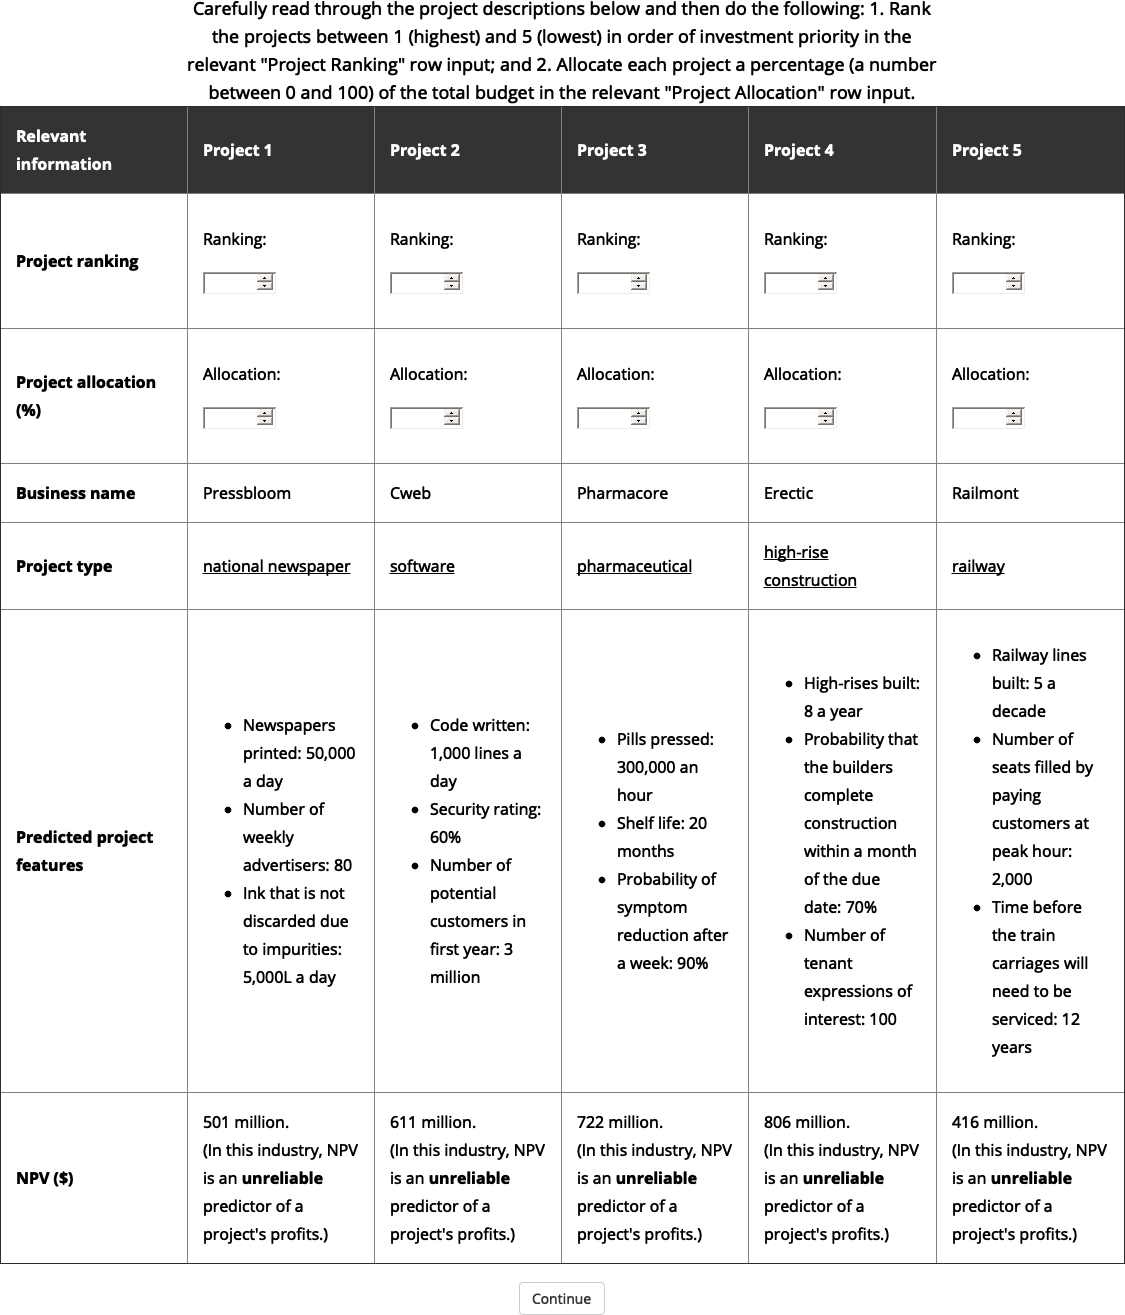
\includegraphics[width=1\linewidth]{project-similarity-bias-and-variance-neglect_files/figure-latex/projects-alignment-low-reliability-explicit-low-materials-alignment-8-1} \caption{An example of a low alignment, low verbal reliability display in Experiment~3.}\label{fig:projects-alignment-low-reliability-explicit-low-materials-alignment-8}
\end{figure}



\begin{figure}
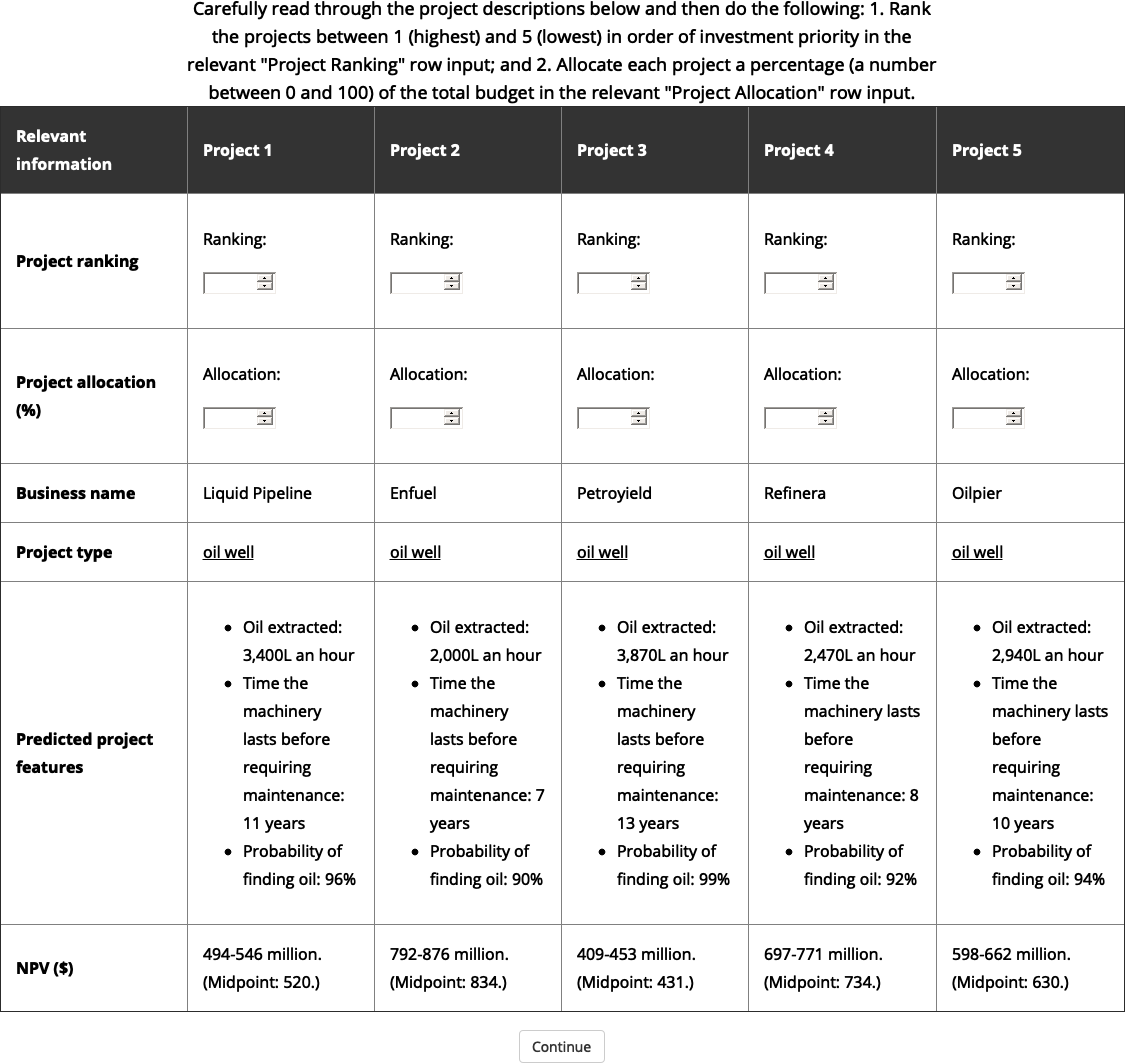
\includegraphics[width=1\linewidth]{project-similarity-bias-and-variance-neglect_files/figure-latex/projects-alignment-high-reliability-implicit-high-materials-alignment-8-1} \caption{An example of a high alignment, high numerical reliability display in Experiment~3.}\label{fig:projects-alignment-high-reliability-implicit-high-materials-alignment-8}
\end{figure}

Three elements were counterbalanced: (a) the association between reliability
level and project set (two variations), (b) the association between business
name and NPV (five latin square variations), and (c) project variation (five
variations per alignment condition). When counterbalancing for the high
alignment group, projects varied by project type (e.g., whether the five
projects all described oil wells or microchips). When counterbalancing for the
low alignment group, projects varied by their intrinsic features (e.g., whether
the oil well project in the set indicated a probability of finding oil of 96\% or
90\%). Table column order and project display order were both randomised.

\hypertarget{interstitial-page}{%
\paragraph{Interstitial Page}\label{interstitial-page}}

Prior to each project being displayed, participants were shown an interstitial
page, which was used to (a) introduce the next display, and (b) check the
participant's attention (given that no input was required, participants could
easily skip the page without reading the text). See
Appendix~\ref{interstitial-materials-alignment-8} for an example.

\hypertarget{results-1}{%
\subsection{Results}\label{results-1}}

A mixed factorial ANOVA was conducted to investigate the effects of NPV, project
alignment, NPV reliability level, and NPV reliability type on participants'
project allocations (see Figure~\ref{fig:plot-alignment-8-allocation} for the
main results and Appendix~\ref{results-alignment-8-allocation} for the
remainder of the hypothesised allocation effects). The four-way interaction
(alignment \(\times\) reliability level \(\times\) NPV \(\times\) reliability type)
was not significant, \(F(3.20, 1,420.19) = 0.71\), \(p = .555\), \(\hat{\eta}^2_p = .002\). Regardless,
the primary hypotheses were supported.

\hypertarget{verbal-reliability}{%
\subsubsection{Verbal Reliability}\label{verbal-reliability}}

The three-way interaction (alignment \(\times\) reliability level \(\times\) NPV
amount) in the verbal reliability condition was not significant,
\(\Delta M = 13.42\), 95\% CI \([-1.27, 28.11]\), \(t(444) = 1.80\), \(p = .073\). This is
because NPV reliability level interacted with NPV in both alignment conditions.
This is a different pattern from Experiment~1 where there was no effect of NPV
reliability level in the low alignment condition. In the high alignment
condition, the interaction between the linear NPV trend and NPV reliability
level was significant,
\(\Delta M = -36.63\), 95\% CI \([-47.02, -26.25]\), \(t(444) = -6.93\), \(p < .001\).
Specifically, the trend was stronger for the high reliability condition,
\(\Delta M = 27.26\), 95\% CI \([17.69, 36.83]\), \(t(444) = 5.60\), \(p < .001\),
compared with the low reliability condition,
\(\Delta M = -9.38\), 95\% CI \([-18.86, 0.11]\), \(t(444) = -1.94\), \(p = .053\).
This shows that, similar to Experiment~1, participants' allocations depended on
verbally expressed NPV reliability. In low alignment, there was also an
interaction between the linear NPV trend and NPV reliability level,
\(\Delta M = -23.21\), 95\% CI \([-33.60, -12.83]\), \(t(444) = -4.39\), \(p < .001\).
This suggests that allocations also depended on verbal reliability in the low
alignment condition.

However, another aspect of the data suggests a greater use of NPV in the low
alignment condition. The linear NPV trend was stronger in the low
alignment condition than in the high alignment condition when averaged over
reliability level,
\(\Delta M = 28.97\), 95\% CI \([17.68, 40.26]\), \(t(444) = 5.04\), \(p < .001\). This
suggests that when NPV reliability was expressed verbally, similar to
Experiment~1, participants relied more on NPV when projects were dissimilar than
when they were similar.

Overall, participants used NPV less when it was described as less reliable in
both high and low alignment conditions, and further, used NPV more when projects
were less alignable regardless of how reliable NPV was described to be.

\hypertarget{numerical-reliability}{%
\subsubsection{Numerical Reliability}\label{numerical-reliability}}

The numerical reliability data were analysed differently to the verbal
reliability data because the effects of interest here were the alignment and
reliability level effects. The linear NPV trend was stronger in the low
alignment condition, averaged over reliability level (with Bonferroni
adjustment),
\(\Delta M = 15.19\), \(95\%\ \mathrm{CI}_\mathrm{\scriptsize Bonferroni(5)}\) \([0.78, 29.60]\), \(t(444) = 2.64\), \(p_\mathrm{\scriptsize Bonferroni(5)} = .034\). This
pattern was the same as that found for the verbal reliability condition above
and in Experiment~2. Further, the linear NPV trend was not significantly
different between the reliability level conditions for both the low alignment
condition,
\(\Delta M = 1.64\), \(95\%\ \mathrm{CI}_\mathrm{\scriptsize Bonferroni(5)}\) \([-11.61, 14.90]\), \(t(444) = 0.31\), \(p_\mathrm{\scriptsize Bonferroni(5)} > .999\),
and high alignment condition,
\(\Delta M = -1.21\), \(95\%\ \mathrm{CI}_\mathrm{\scriptsize Bonferroni(5)}\) \([-14.46, 12.05]\), \(t(444) = -0.23\), \(p_\mathrm{\scriptsize Bonferroni(5)} > .999\).
This indicates that participants did not use numerical NPV reliability to inform
their allocations.



\begin{figure}[!htbp]
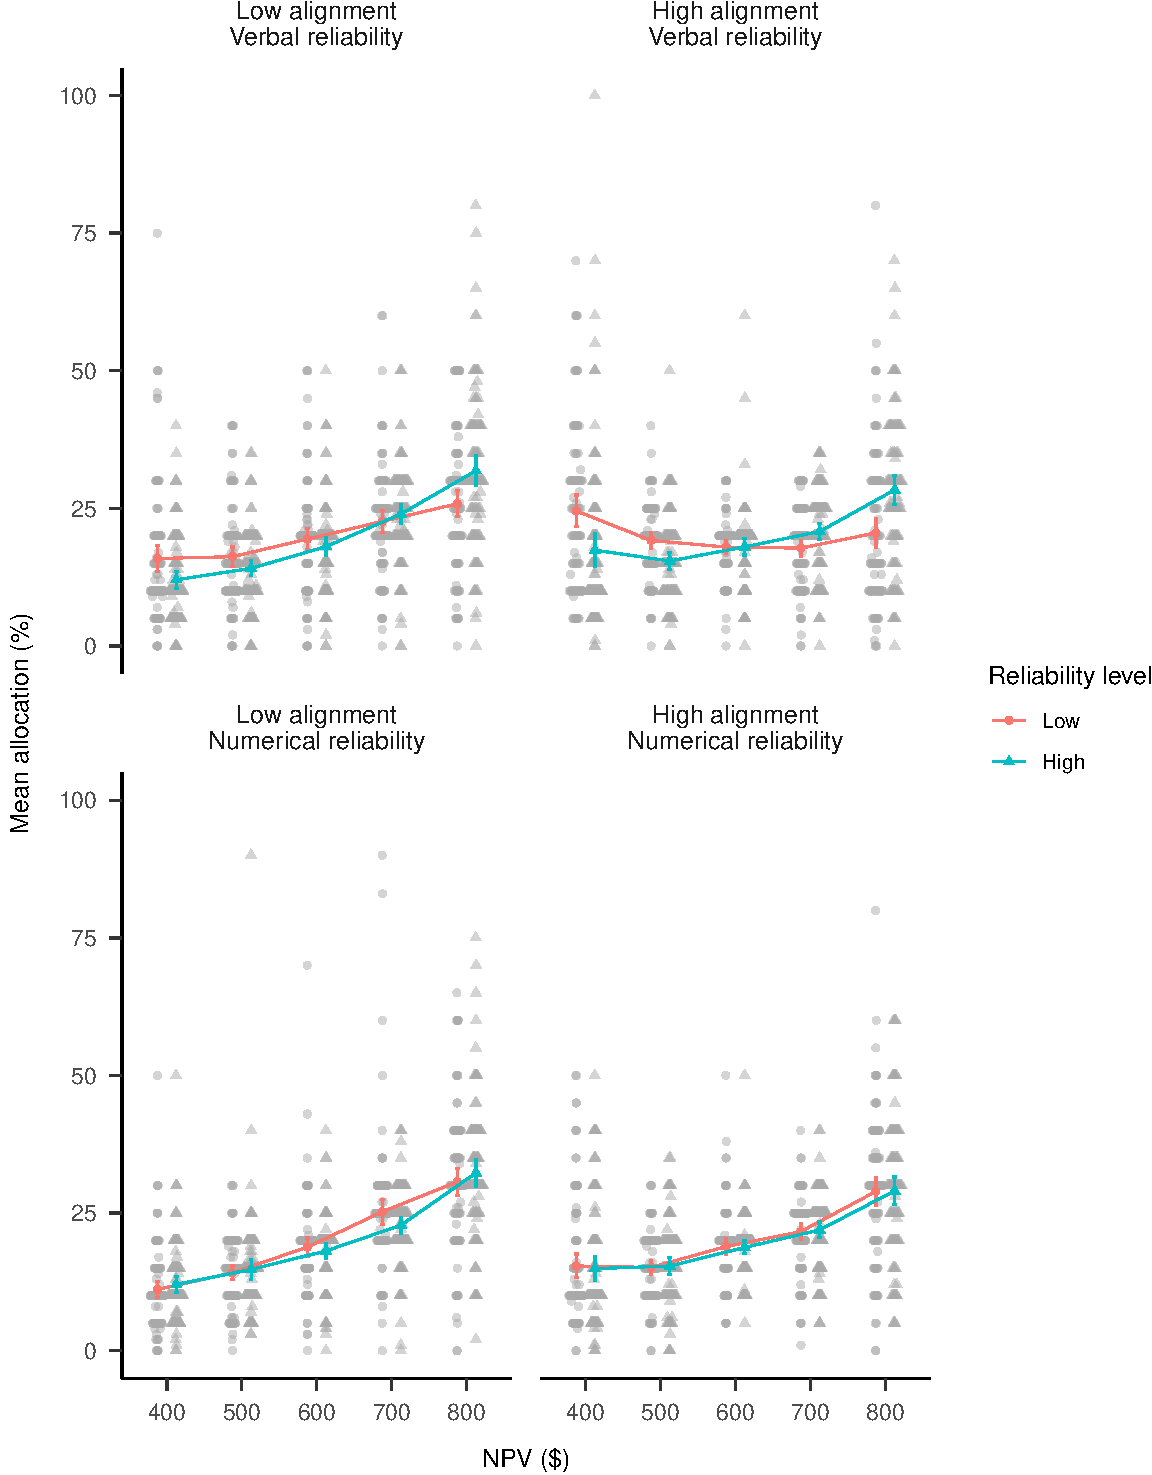
\includegraphics[width=1\linewidth]{project-similarity-bias-and-variance-neglect_files/figure-latex/plot-alignment-8-allocation-1} \caption{Mean allocation across NPV, by alignment, reliability level, and reliability type conditions. Error bars represent 95\% confidence intervals, calculated from the within-subjects standard errors using the method from Cousineau and O'Brien (\protect\hyperlink{ref-cousineau2014}{2014}). Raw data are plotted in the background.}\label{fig:plot-alignment-8-allocation}
\end{figure}

Similar to the verbal reliability condition, the use of NPV was stronger in the
low alignment condition than it was in the high alignment condition. However,
unlike the verbal reliability condition, allocations did not depend on numerical
reliability in either the low or the high alignment condition. In the verbal
reliability condition, allocations depended on NPV reliability level in both
alignment conditions.

\hypertarget{discussion-2}{%
\subsection{Discussion}\label{discussion-2}}

Hypotheses~\ref{hyp:three-way-alignment-2},~\ref{hyp:allocation-alignment-alignment-2},~\ref{hyp:allocation-alignment-reliability-npv-alignment-2},
and~\ref{hyp:allocation-alignment-high-alignment-2} were supported in the
verbal reliability condition. This shows that, while overall participants
preferred to use NPV as a proxy for project quality in their allocations, they
still used verbal reliability information. Specifically, when projects were
similar, participants used NPV when they were told that it was reliable, and
used alternative metrics when told that it was not reliable. However, in
Experiment~3, no support was found for
Hypothesis~\ref{hyp:allocation-alignment-low-alignment-2}. It was expected that
participants in the low alignment condition would use NPV regardless of the
reliability level conditions, as in Experiment~1. Rather, they used NPV less
when told that it was unreliable. However, they primarily used NPV overall, as
shown by the positive NPV trend in both reliability level conditions.

Further, Experiment~3 replicated the finding of Experiment~2 for the numerical
reliability condition. Specifically, participants relied more on NPV when
projects were dissimilar but, critically, did not use numerical range
information to influence their allocations. A pilot study (Dekel, \protect\hyperlink{ref-dekel2021b}{2021},
Appendix B.8) replicated the results of Experiment~1 in the verbal reliability
condition, but did not replicate the results of Experiment~2 in the numerical
reliability condition. That is, when faced with numerical ranges as the NPV
reliability information, participants did not even use the midpoint in their
decisions. The results of Experiment~3 suggest that the finding in the pilot
experiment may have been spurious or due to an unexplored component of the
experimental design, but this can only be deteremined with future research.

\hypertarget{general-discussion}{%
\section{General Discussion}\label{general-discussion}}

Across three experiments there were two main findings: (a) NPV is used more when
options are difficult to compare in the low alignment conditions; and (b) people
do not consider numerical variance information, despite this being important to
the reliability of the NPV forecasts. This pattern with numerical reliability
information contrasted with the frequent use of verbal indicators of reliability
level. This numerical variance neglect is surprising, since other work showed
that people can readily extract variance information when experiencing numerical
sequences (Rosenbaum et al., \protect\hyperlink{ref-rosenbaum2020}{2020}). Both the verbal and numerical effects were
consistent for both naive and experienced participants, indicating their
persistence. People make use of metrics with alignable differences when required
to compare disparate options. However, they do not always use alternative
metrics, even when they are available.

Experiment~1 found that participants did not use NPV in their allocation
decisions when they were told that it was unreliable but did use it when told it
was reliable. Experiment~2 found that participants with some business experience
relied more on NPV for capital allocation when the rest of the information was
non-alignable compared with when it was alignable. However, they did not take
into account numerical reliability information when making these decisions.
Experiment~3 found further evidence of these effects within one experimental
design.

Alignable differences have been shown to be important into decision-making in
many settings (Markman \& Loewenstein, \protect\hyperlink{ref-markman2010}{2010}; Markman \& Medin, \protect\hyperlink{ref-markman1995}{1995}). The experiments presented in the
present study are novel in terms of the effects of project alignment on capital
allocation. Further, these experiments considered the extent to which the
reliability of an alignable measure (NPV) affects the way in which it is used.
This depended on the availability of other alignable differences in the set of
choices. If other alignable differences were available, then participants were
willing to reduce their use of a reportedly unreliable alignable measure (or use
it when told that it was reliable). However, when no other alignable differences
were available, then the alignable, albeit unreliable, measure was more likely
to be used. This was found in both Experiments~1 and~3, as well as in a pilot
study to a lesser extent (reported in Dekel, \protect\hyperlink{ref-dekel2021b}{2021}, Appendix B.4).

Financial measures such as NPV are useful because of their alignability. That
is, they may serve as an alignable difference, regardless of the inherent
similarities between a set of projects. Psychologically, these measures are
useful because they allow for relevant inferences (Lassaline, \protect\hyperlink{ref-lassaline1996}{1996}) and because
they offer an abstraction of concrete details (Doumas \& Hummel, \protect\hyperlink{ref-doumas2013}{2013}). However, the
structural alignment account does not directly speak to real-world implications
when there is a need for non-alignable comparisons. NPV is a type of abstraction
that facilitates the comparison of different aspects of a company. For instance,
the use of NPV may facilitate the comparison of an oil field project with a
refinery project. However, this increased alignment could actually hide
important information because it does not consider the finer complexities
inherent in each business unit. The forecasts used to calculate NPV for each
business unit are based on different indicators, and there are likely to be
differences between each unit's estimates. Thus, one can imagine a continuum of
comparisons in which the usefulness of comparison increases with the level of
alignability but depends on the level of abstraction that is required to achieve
the alignment.

The finding that participants, even those with some business experience, did not
sufficiently consider variance information is surprising but understandable. It
is surprising because financial decision-making largely depends on the
consideration of different sources of variance (e.g., risk, volatility, and
uncertainty). At the same time, it is understandable because research from
psychology and statistics education shows that statistics students and people in
general have a poor ability to draw statistical inferences (e.g., Galesic \& Garcia-Retamero, \protect\hyperlink{ref-galesic2010}{2010}; Konold et al., \protect\hyperlink{ref-konold1993}{1993}). Future research should investigate the conditions under which
individuals' sensitivity to variance information may be facilitated. For
instance, it is unclear whether it is merely salience that is lacking, meaning
that visual aids could be useful, or whether a further explicit explanation of
statistical inference is necessary. The findings of a pilot experiment suggest
that participants struggle to use numerical NPV reliability information, even
when given explicit instructions (Dekel, \protect\hyperlink{ref-dekel2021b}{2021}, Appendix B.7).

A possible limitation of these experiments is the use of NPV as the only
financial metric. In the business world, there are many metrics that serve
similar functions and are used as tools to deal with non-alignable options.
Therefore, future research should attempt to replicate the current findings
using different financial measures.

Future research should also investigate the boundary conditions of the
reliability type effect. That is, people appear to respond to explicit
reliability information but not to variance information that only implies
reliability. Future research should attempt to identify the minimal variance
information that participants need to understand the relevant implications for
reliability. Participants may simply not notice the variance information or
assume that it is irrelevant. For instance, future research could test
participants in a condition in which the variance information is more salient.

\newpage

\newpage

\hypertarget{references}{%
\section{References}\label{references}}

\begingroup
\setlength{\parindent}{-0.5in}
\setlength{\leftskip}{0.5in}

\hypertarget{refs}{}
\begin{cslreferences}
\leavevmode\hypertarget{ref-bardolet2011}{}%
Bardolet, D., Fox, C. R., \& Lovallo, D. (2011). Corporate capital allocation: A behavioral perspective. \emph{Strategic Management Journal}, \emph{32}(13), 1465--1483. \url{https://doi.org/10/cn6xsb}

\leavevmode\hypertarget{ref-batteux2020}{}%
Batteux, E., Bilovich, A., Johnson, S., \& Tuckett, D. (2020). \emph{Impressed by Numbers: The Extent to Which Novice Investors Favor Precise Numerical Information in a Context of Uncertainty} (SSRN Scholarly Paper ID 3595409). Social Science Research Network. \url{https://doi.org/10.2139/ssrn.3595409}

\leavevmode\hypertarget{ref-cousineau2014}{}%
Cousineau, D., \& O'Brien, F. (2014). Error bars in within-subject designs: A comment on Baguley (2012). \emph{Behavior Research Methods}, \emph{46}(4), 1149--1151. \url{https://doi.org/10/f6vdsw}

\leavevmode\hypertarget{ref-dekel2021b}{}%
Dekel, S. (2021). \emph{The Psychology of Managerial Capital Allocation} {[}Doctoral dissertation, The University of Sydney{]}. \url{https://thesis.shirdekel.com/}

\leavevmode\hypertarget{ref-doumas2013}{}%
Doumas, L. A. A., \& Hummel, J. E. (2013). Comparison and Mapping Facilitate Relation Discovery and Predication. \emph{PLoS ONE}, \emph{8}(6), 1--8. \url{https://doi.org/10/gjscsn}

\leavevmode\hypertarget{ref-fox2008}{}%
Fox, R. (2008). A brief critical history of NPV. \emph{BAA Conference}, 16. \url{http://usir.salford.ac.uk/id/eprint/9291/2/NPV_paper.pdf}

\leavevmode\hypertarget{ref-galesic2010}{}%
Galesic, M., \& Garcia-Retamero, R. (2010). Statistical Numeracy for Health: A Cross-cultural Comparison With Probabilistic National Samples. \emph{Arch Intern Med}, \emph{170}(5), 462--468. \url{https://doi.org/10/fmj7q3}

\leavevmode\hypertarget{ref-gentner1983}{}%
Gentner, D. (1983). Structure-Mapping: A Theoretical Framework for Analogy. \emph{Cognitive Science}, \emph{7}(2), 155--170. \url{https://doi.org/10/dw52z8}

\leavevmode\hypertarget{ref-gentner1997}{}%
Gentner, D., \& Markman, A. B. (1997). Structure mapping in analogy and similarity. \emph{American Psychologist}, \emph{52}(1), 45--56. \url{https://doi.org/10/fm4rrb}

\leavevmode\hypertarget{ref-graham2001}{}%
Graham, J. R., \& Harvey, C. R. (2001). The theory and practice of corporate finance: Evidence from the field. \emph{Journal of Financial Economics}, \emph{60}(2), 187--243. \url{https://doi.org/10/fpdzrj}

\leavevmode\hypertarget{ref-graham2015}{}%
Graham, J. R., Harvey, C. R., \& Puri, M. (2015). Capital allocation and delegation of decision-making authority within firms. \emph{Journal of Financial Economics}, \emph{115}(3), 449--470. \url{https://doi.org/10/gfvz8d}

\leavevmode\hypertarget{ref-konold1993}{}%
Konold, C., Pollatsek, A., Well, A., Lohmeier, J., \& Lipson, A. (1993). Inconsistencies in Students' Reasoning about Probability. \emph{Journal for Research in Mathematics Education}, \emph{24}(5), 392. \url{https://doi.org/10/bq4hvm}

\leavevmode\hypertarget{ref-lakens2018}{}%
Lakens, D., Scheel, A. M., \& Isager, P. M. (2018). Equivalence Testing for Psychological Research: A Tutorial. \emph{Advances in Methods and Practices in Psychological Science}, \emph{1}(2), 259--269. \url{https://doi.org/10/gdj7s9}

\leavevmode\hypertarget{ref-lassaline1996}{}%
Lassaline, M. E. (1996). Structural alignment in induction and similarity. \emph{Journal of Experimental Psychology: Learning, Memory, and Cognition}, \emph{22}(3), 754--770. \url{https://doi.org/10/fq9fww}

\leavevmode\hypertarget{ref-long2018}{}%
Long, A. R., Fernbach, P. M., \& De Langhe, B. (2018). Circle of Incompetence: Sense of Understanding as an Improper Guide to Investment Risk. \emph{Journal of Marketing Research}, \emph{55}(4), 474--488. \url{https://doi.org/10/gjscr7}

\leavevmode\hypertarget{ref-lovallo2003}{}%
Lovallo, D., \& Kahneman, D. (2003). Delusions of Success: How Optimism Undermines Executives' Decisions. \emph{Harvard Business Review}, \emph{81}(7).

\leavevmode\hypertarget{ref-markman1993}{}%
Markman, A. B., \& Gentner, D. (1993). Structural Alignment during Similarity Comparisons. \emph{Cognitive Psychology}, \emph{25}(4), 431--467. \url{https://doi.org/10/cqtx7q}

\leavevmode\hypertarget{ref-markman2010}{}%
Markman, A. B., \& Loewenstein, J. (2010). Structural comparison and consumer choice. \emph{Journal of Consumer Psychology}, \emph{20}(2), 126--137. \url{https://doi.org/10/d7b49c}

\leavevmode\hypertarget{ref-markman1995}{}%
Markman, A. B., \& Medin, D. L. (1995). Similarity and Alignment in Choice. \emph{Organizational Behavior and Human Decision Processes}, \emph{63}(2), 117--130. \url{https://doi.org/10/c8z7r9}

\leavevmode\hypertarget{ref-puri2007}{}%
Puri, M., \& Robinson, D. T. (2007). Optimism and economic choice. \emph{Journal of Financial Economics}, \emph{86}(1), 71--99. \url{https://doi.org/10/c9839j}

\leavevmode\hypertarget{ref-remer1993}{}%
Remer, D. S., Stokdyk, S. B., \& Van Driel, M. (1993). Survey of project evaluation techniques currently used in industry. \emph{International Journal of Production Economics}, \emph{32}(1), 103--115. \url{https://doi.org/10/bsc6bs}

\leavevmode\hypertarget{ref-rosenbaum2020}{}%
Rosenbaum, D. M., Glickman, M., \& Usher, M. (2020). \emph{Extracting summary statistics of rapid numerical sequences} {[}Preprint{]}. PsyArXiv. \url{https://doi.org/10.31234/osf.io/6scav}

\leavevmode\hypertarget{ref-vivalt2021}{}%
Vivalt, E., \& Coville, A. (2021). \emph{How Do Policy-Makers Update Their Beliefs?} (p. 51). \url{http://evavivalt.com/wp-content/uploads/How-Do-Policymakers-Update.pdf}

\leavevmode\hypertarget{ref-willigers2017}{}%
Willigers, B. J. A., Jones, B., \& Bratvold, R. B. (2017). The Net-Present-Value Paradox: Criticized by Many, Applied by All. \emph{SPE Economics \& Management}, \emph{9}(04), 090--102. \url{https://doi.org/10/gjscsx}
\end{cslreferences}

\endgroup

\hypertarget{appendix-appendix}{%
\appendix}


\hypertarget{alignment-2-appendix}{%
\section{Experiment 1}\label{alignment-2-appendix}}

\hypertarget{instructions-materials-alignment-2-appendix}{%
\subsection{Instructions}\label{instructions-materials-alignment-2-appendix}}

Figures~\ref{fig:instructions-reliability-low-alignment-2},~\ref{fig:instructions-reliability-high-alignment-2},
and~\ref{fig:instructions-reliability-no-npv-alignment-2} show the instructions
given to those in the low NPV reliability, high NPV reliability, and no NPV
condition, respectively.



\begin{figure}
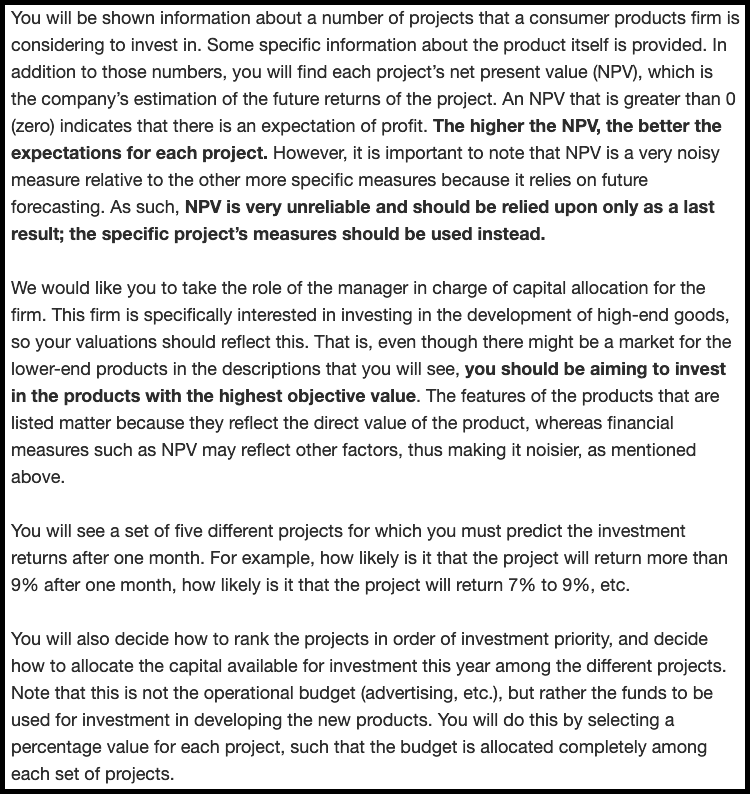
\includegraphics[width=1\linewidth]{project-similarity-bias-and-variance-neglect_files/figure-latex/instructions-reliability-low-alignment-2-1} \caption{Experiment~1 low reliability instructions.}\label{fig:instructions-reliability-low-alignment-2}
\end{figure}



\begin{figure}
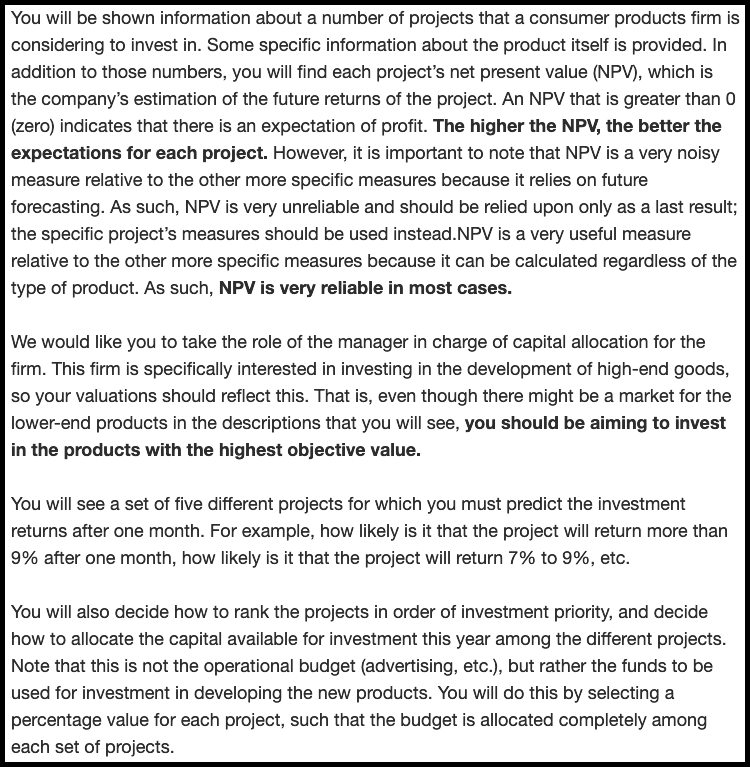
\includegraphics[width=1\linewidth]{project-similarity-bias-and-variance-neglect_files/figure-latex/instructions-reliability-high-alignment-2-1} \caption{Experiment~1 high reliability instructions.}\label{fig:instructions-reliability-high-alignment-2}
\end{figure}



\begin{figure}
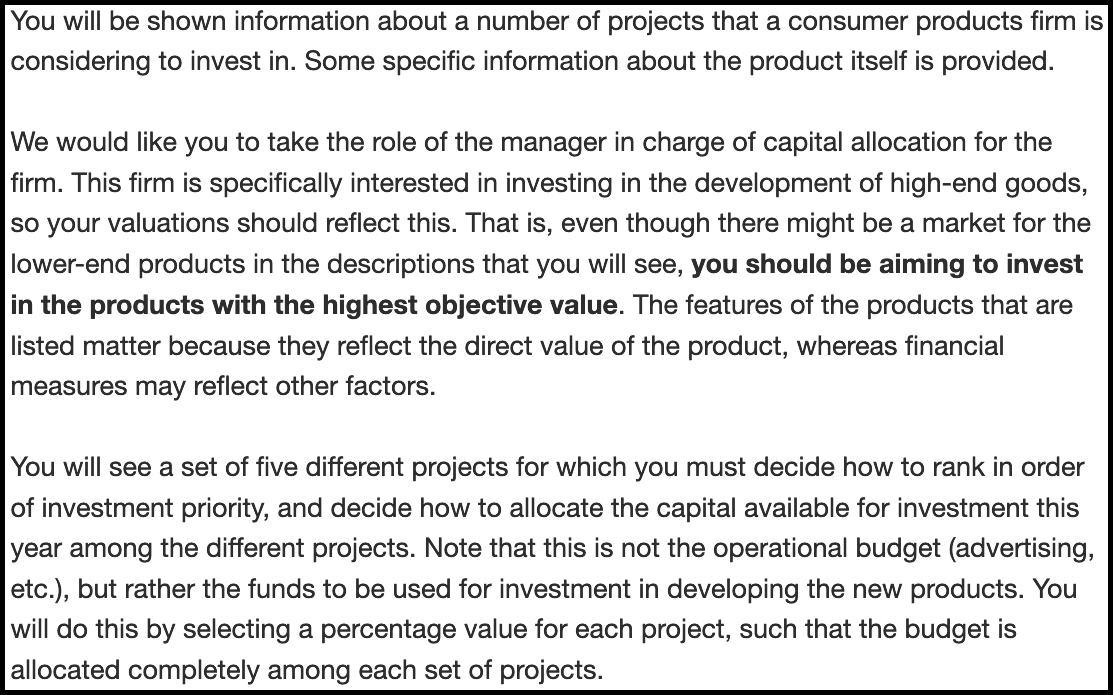
\includegraphics[width=1\linewidth]{project-similarity-bias-and-variance-neglect_files/figure-latex/instructions-reliability-no-npv-alignment-2-1} \caption{The instructions for the no NPV condition in Experiment~1.}\label{fig:instructions-reliability-no-npv-alignment-2}
\end{figure}

\hypertarget{forecasting-materials-alignment-2}{%
\subsection{Forecasting}\label{forecasting-materials-alignment-2}}

Participants were asked to respond to a forecasting task (adapted from Long et al., \protect\hyperlink{ref-long2018}{2018}), seen in Figure~\ref{fig:forecasting-materials-alignment-2}.
Participants were asked to predict each project's rate of return after one
month. This allowed to calculate each participant's forecasting mean and
standard deviation (the latter as inversely proportional to forecasting
precision).



\begin{figure}
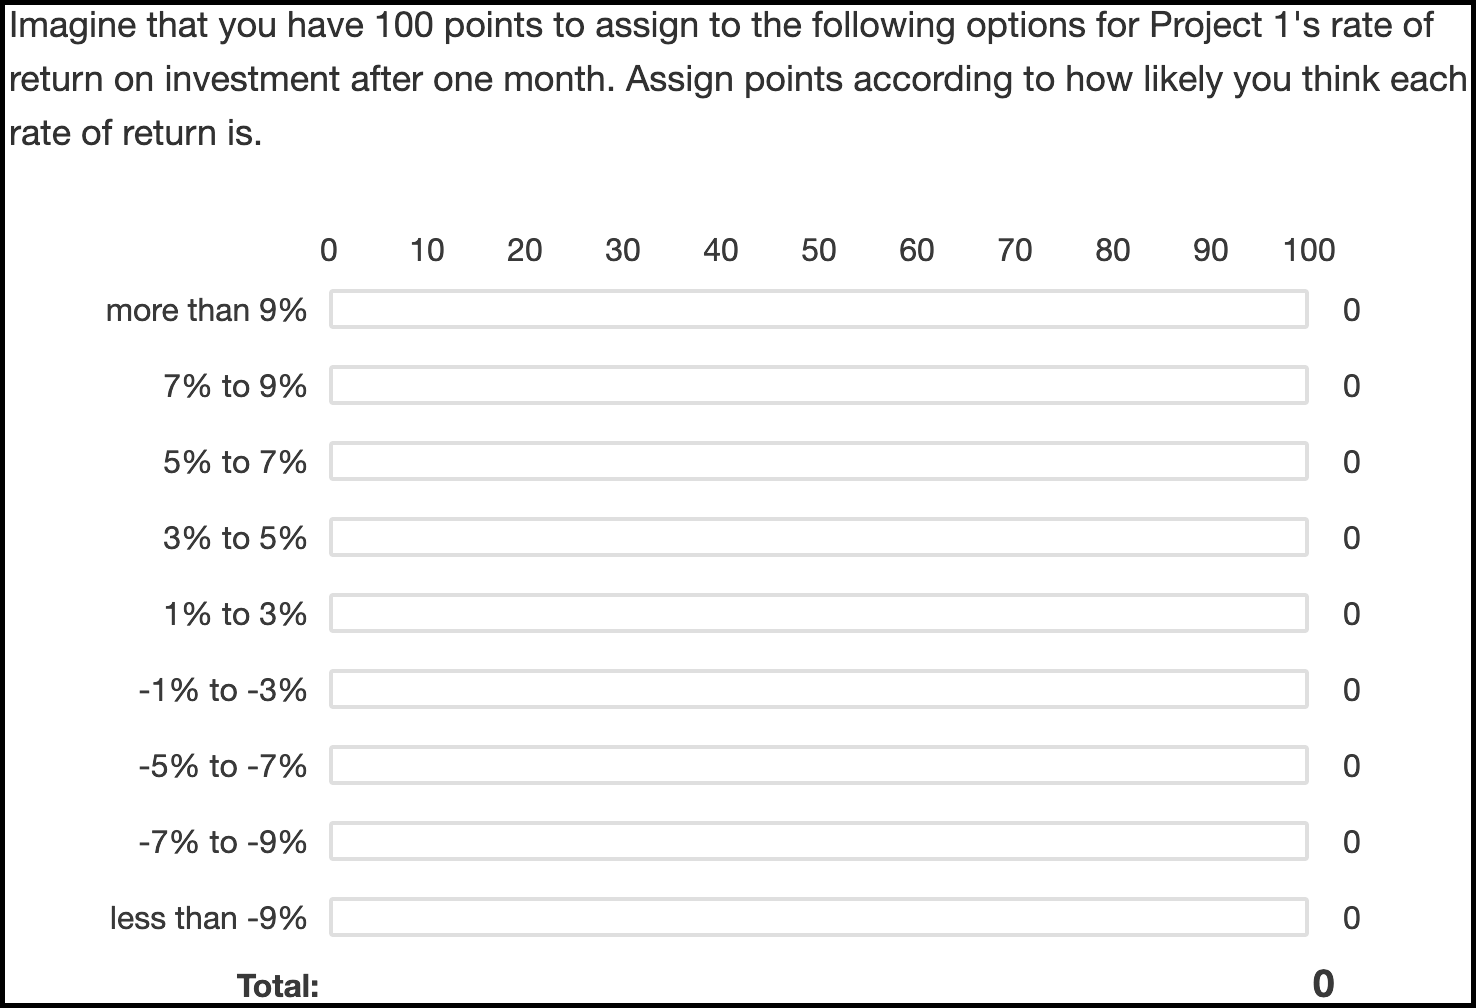
\includegraphics[width=1\linewidth]{project-similarity-bias-and-variance-neglect_files/figure-latex/forecasting-materials-alignment-2-1} \caption{The forecasting task.}\label{fig:forecasting-materials-alignment-2}
\end{figure}

\hypertarget{ranking-materials-alignment-2}{%
\subsection{Ranking}\label{ranking-materials-alignment-2}}

As shown in Figure~\ref{fig:ranking-materials-alignment-2}, participants were
asked to rank the projects in order of investment priority.



\begin{figure}
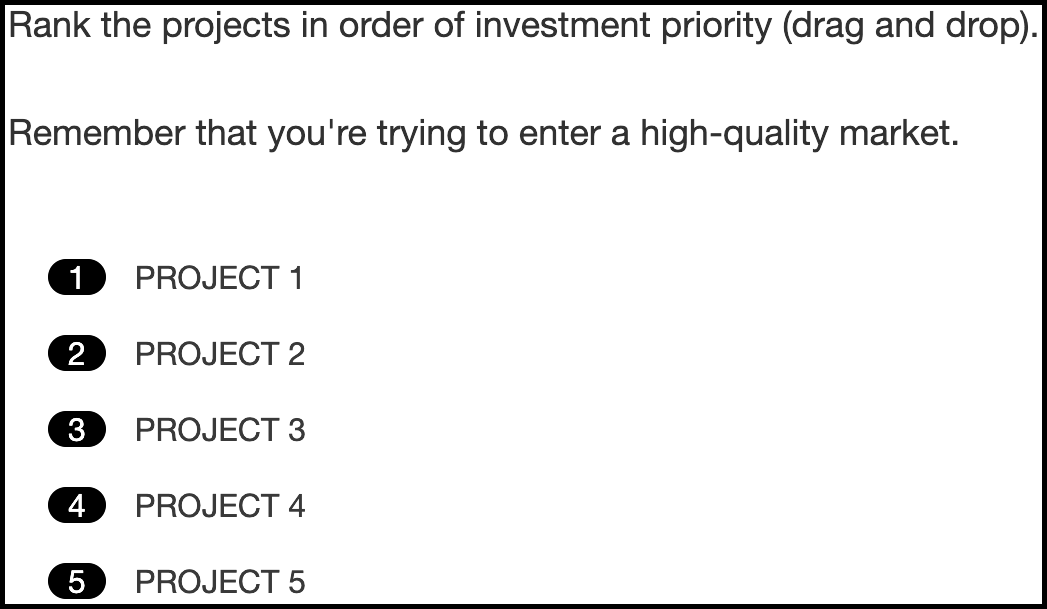
\includegraphics[width=1\linewidth]{project-similarity-bias-and-variance-neglect_files/figure-latex/ranking-materials-alignment-2-1} \caption{The ranking task.}\label{fig:ranking-materials-alignment-2}
\end{figure}

\hypertarget{confidence-materials-alignment-2}{%
\subsection{Confidence}\label{confidence-materials-alignment-2}}

As Figure~\ref{fig:confidence-materials-alignment-2} shows, participants were
asked to indicate how confident they were about each of their allocation
decisions on a scale from 0 (``Not confident at all'') to 100 (``Extremely
confident'').



\begin{figure}
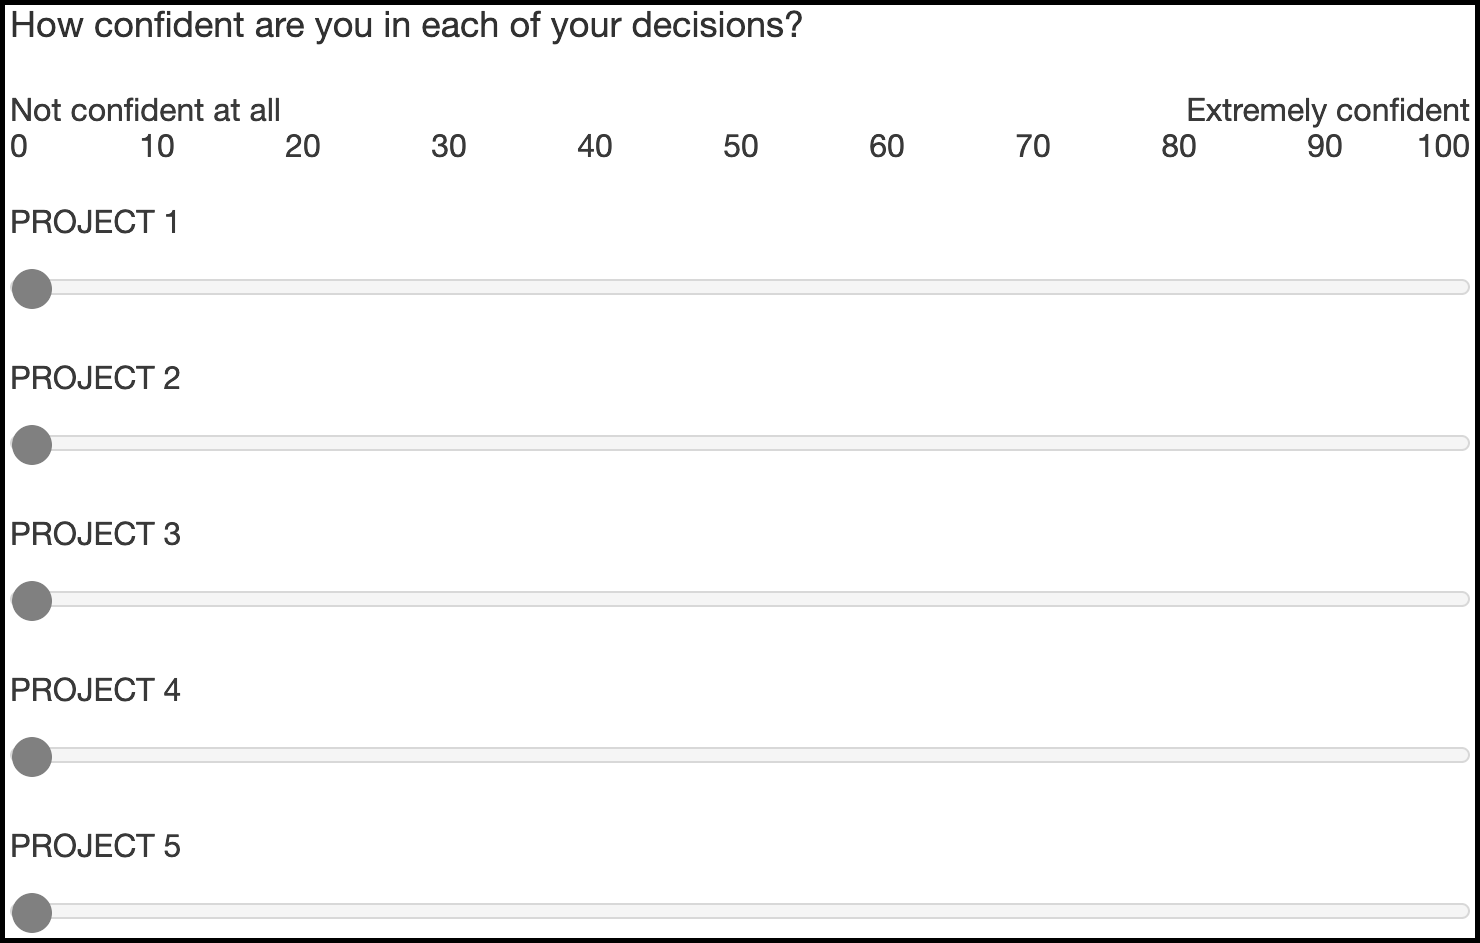
\includegraphics[width=1\linewidth]{project-similarity-bias-and-variance-neglect_files/figure-latex/confidence-materials-alignment-2-1} \caption{The confidence task.}\label{fig:confidence-materials-alignment-2}
\end{figure}

\hypertarget{justification-materials-alignment-2}{%
\subsection{Justification}\label{justification-materials-alignment-2}}

As Figure~\ref{fig:justification-materials-alignment-2} shows, participants
were asked to justify their allocation decision in a free-response text-box.



\begin{figure}
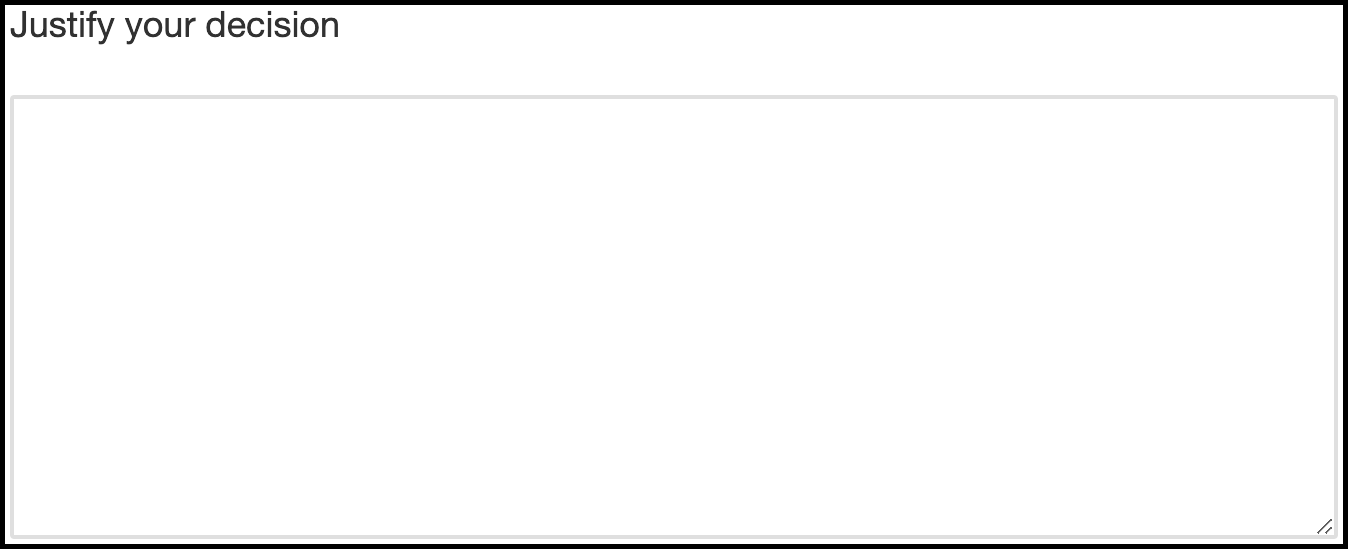
\includegraphics[width=1\linewidth]{project-similarity-bias-and-variance-neglect_files/figure-latex/justification-materials-alignment-2-1} \caption{The justification task.}\label{fig:justification-materials-alignment-2}
\end{figure}

\hypertarget{results-alignment-2-appendix}{%
\subsection{Additional Analyses}\label{results-alignment-2-appendix}}

\hypertarget{ranking}{%
\subsubsection{Ranking}\label{ranking}}

A mixed factorial ANOVA was conducted to investigate the effects of alignment
and verbally-instructed NPV reliability on participants' rankings of the
target project. As shown in Figure~\ref{fig:plot-alignment-2-ranking}, the
alignment \(\times\) reliability level \(\times\) NPV interaction was
significant,
\(F(6.62, 370.54) = 2.70\), \(p = .011\), \(\hat{\eta}^2_p = .046\). This
effect seems to be driven by the differences between the no NPV condition and
the conditions with NPV across the two alignment conditions. Specifically, in
the low alignment condition, the linear NPV trend was significantly lower in the
no NPV condition than both the low reliability condition,
\(\Delta M = -6.56\), 95\% CI \([-10.26, -2.85]\), \(t(112) = -3.50\), \(p = .001\), and the high
reliability condition, \(\Delta M = -7.38\), 95\% CI \([-10.83, -3.93]\), \(t(112) = -4.24\), \(p < .001\).
However, in the high alignment condition, the linear NPV trend was only
significantly lower in the no NPV condition than the high reliability condition,
\(\Delta M = -8.37\), 95\% CI \([-11.85, -4.88]\), \(t(112) = -4.76\), \(p < .001\), and not the low
reliability condition, \(\Delta M = -1.71\), 95\% CI \([-5.54, 2.13]\), \(t(112) = -0.88\), \(p = .380\).



\begin{figure}
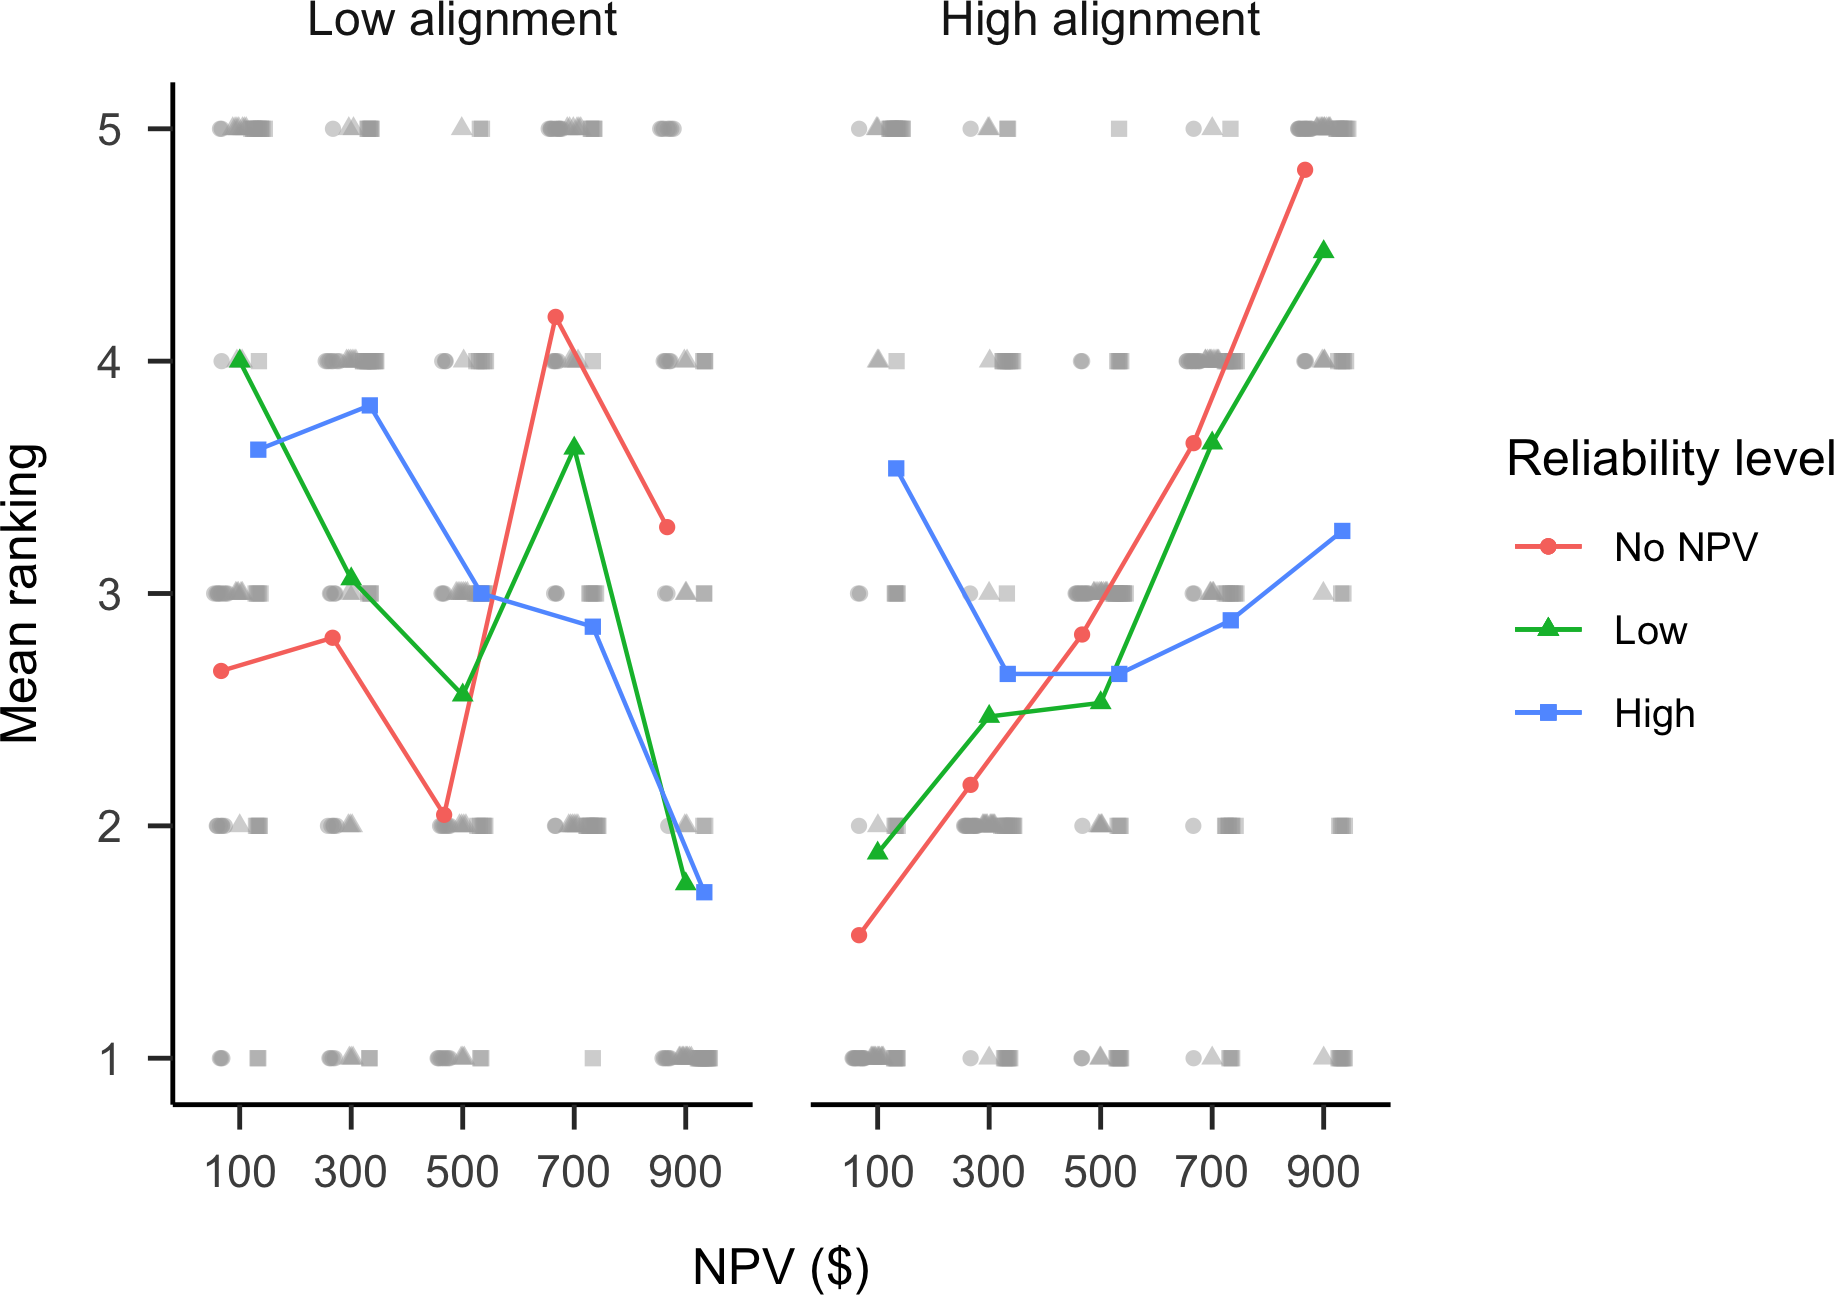
\includegraphics[width=1\linewidth]{project-similarity-bias-and-variance-neglect_files/figure-latex/plot-alignment-2-ranking-1} \caption{Mean ranking.}\label{fig:plot-alignment-2-ranking}
\end{figure}

\hypertarget{confidence}{%
\subsubsection{Confidence}\label{confidence}}

A mixed factorial ANOVA was conducted to investigate the effects of alignment
and verbally-instructed NPV reliability on participants' confidence rating of
their decisions. As shown in Figure~\ref{fig:plot-alignment-2-confidence}, the
alignment \(\times\) reliability level \(\times\) NPV interaction was not
significant,
\(F(7.47, 418.08) = 1.26\), \(p = .267\), \(\hat{\eta}^2_p = .022\).
Contrary to the allocation and ranking data, in
the low alignment condition, there were no significant differences in the linear
NPV trend between the no NPV condition and low reliability condition,
\(\Delta M = 10.73\), 95\% CI \([-30.15, 51.61]\), \(t(112) = 0.52\), \(p = .604\), nor the high
reliability condition, \(\Delta M = 13.05\), 95\% CI \([-24.97, 51.07]\), \(t(112) = 0.68\), \(p = .498\).
However, as above, in the high alignment condition, the linear NPV trend was
significantly lower in the no NPV condition than the high reliability condition,
\(\Delta M = 65.14\), 95\% CI \([26.72, 103.57]\), \(t(112) = 3.36\), \(p = .001\), and not the low
reliability condition, \(\Delta M = 31.88\), 95\% CI \([-10.38, 74.14]\), \(t(112) = 1.49\), \(p = .138\).



\begin{figure}
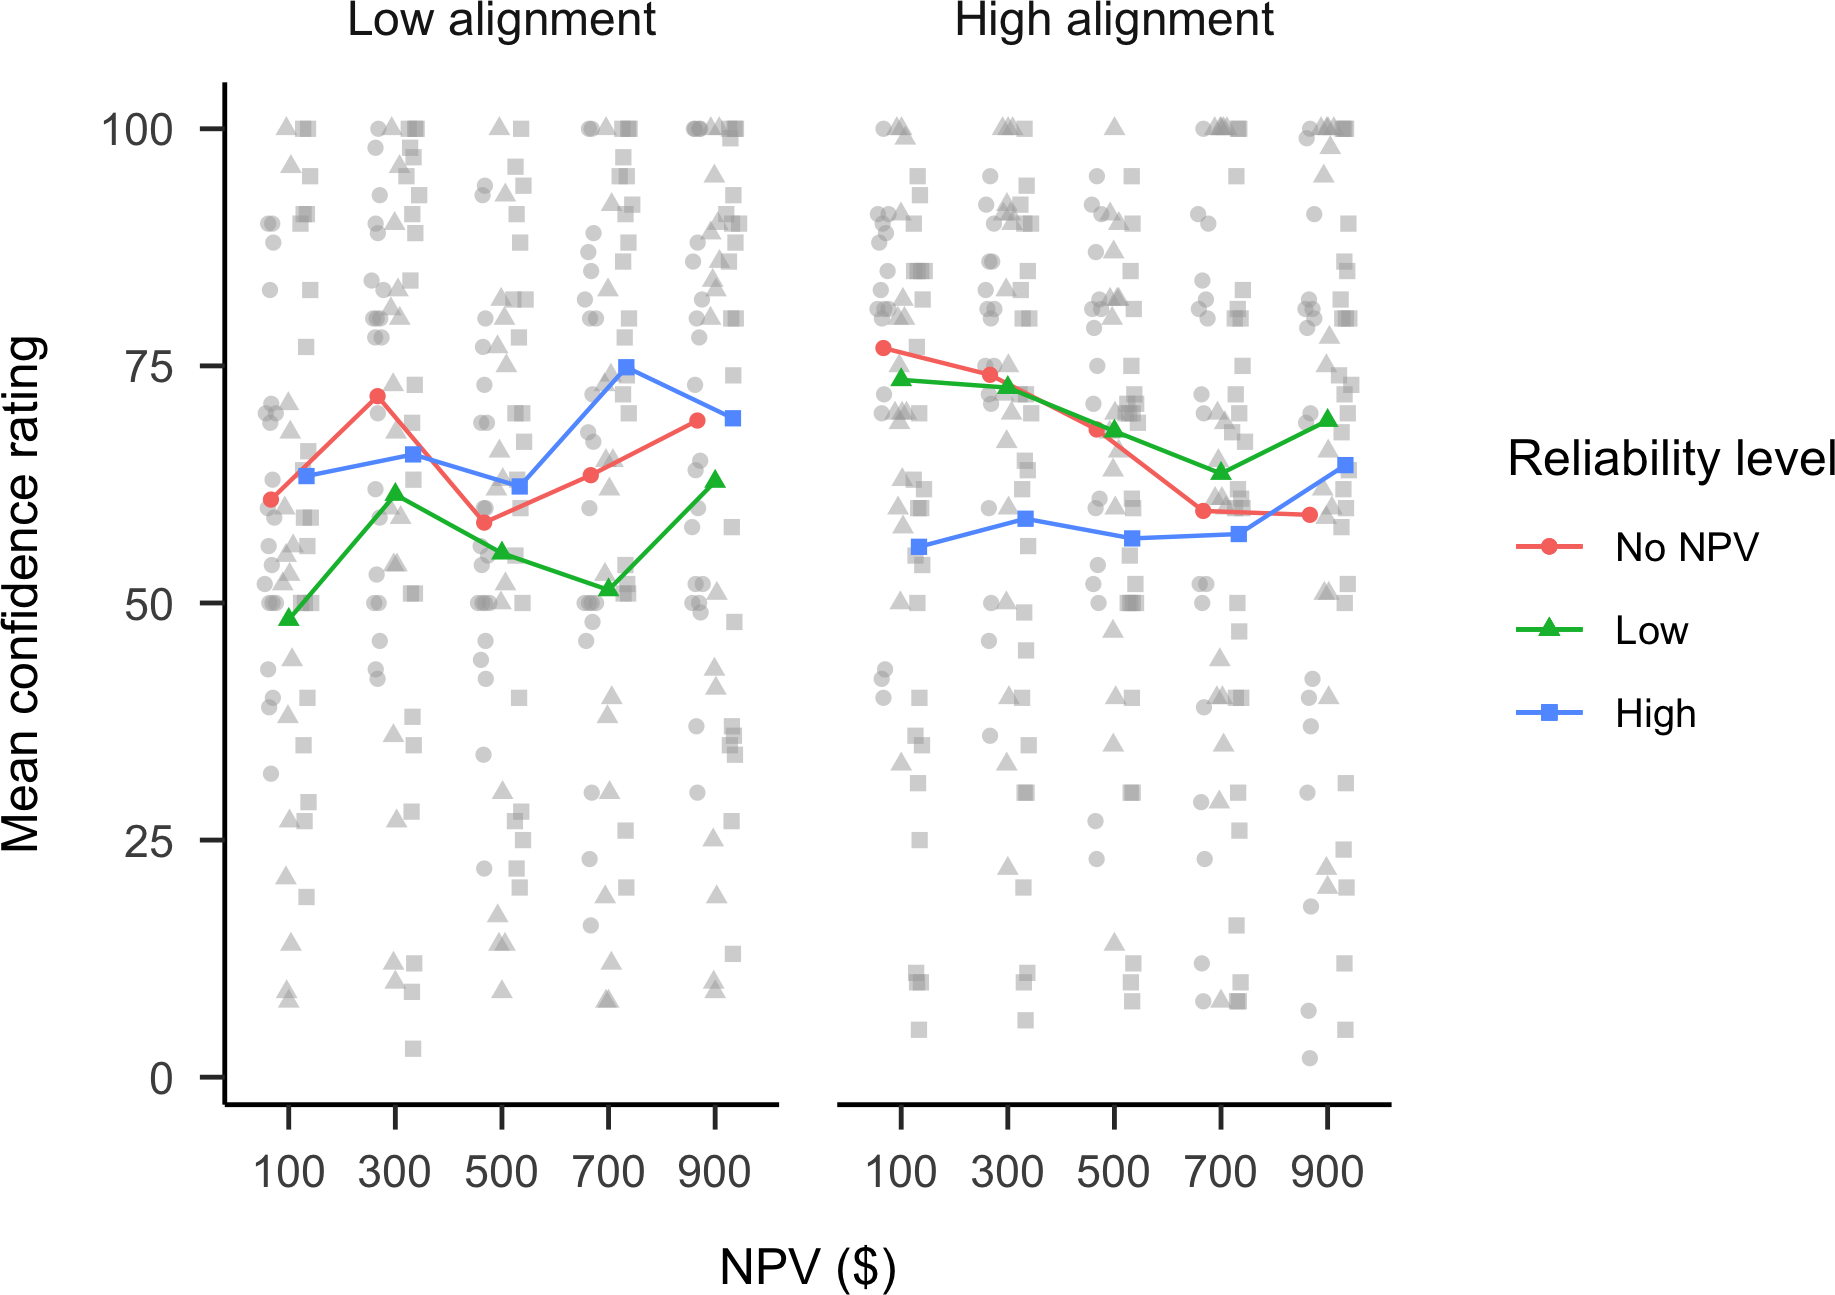
\includegraphics[width=1\linewidth]{project-similarity-bias-and-variance-neglect_files/figure-latex/plot-alignment-2-confidence-1} \caption{Mean confidence.}\label{fig:plot-alignment-2-confidence}
\end{figure}

\hypertarget{forecast-mean}{%
\subsubsection{Forecast Mean}\label{forecast-mean}}

A mixed factorial ANOVA was conducted to investigate the effects of alignment
and verbally-instructed NPV reliability on participants' forecast means. As seen
in Figure~\ref{fig:plot-alignment-2-forecast-mean}, the alignment \(\times\)
reliability level \(\times\) NPV interaction was not significant,
\(F(5.26, 142.10) = 1.89\), \(p = .095\), \(\hat{\eta}^2_p = .066\).
However, the alignment \(\times\) NPV interaction was significant,
\(F(2.63, 142.10) = 2.89\), \(p = .044\), \(\hat{\eta}^2_p = .051\); as well as the
reliability level \(\times\) NPV interaction,
\(F(5.26, 142.10) = 7.91\), \(p < .001\), \(\hat{\eta}^2_p = .227\). The simple
effects appear to be as above. Specifically, in the low alignment condition, the
linear NPV trend was significantly lower in the no NPV condition than both the
low reliability condition,
\(\Delta M = 0.19\), 95\% CI \([0.09, 0.30]\), \(t(54) = 3.63\), \(p = .001\), and the high
reliability condition,
\(\Delta M = 0.16\), 95\% CI \([0.04, 0.28]\), \(t(54) = 2.75\), \(p = .008\). However, in the
high alignment condition, the linear NPV trend was only significantly lower in
the no NPV condition than the high reliability condition,
\(\Delta M = 0.22\), 95\% CI \([0.11, 0.32]\), \(t(54) = 4.04\), \(p < .001\), and not the low
reliability condition,
\(\Delta M = 0.08\), 95\% CI \([-0.04, 0.21]\), \(t(54) = 1.30\), \(p = .198\).



\begin{figure}
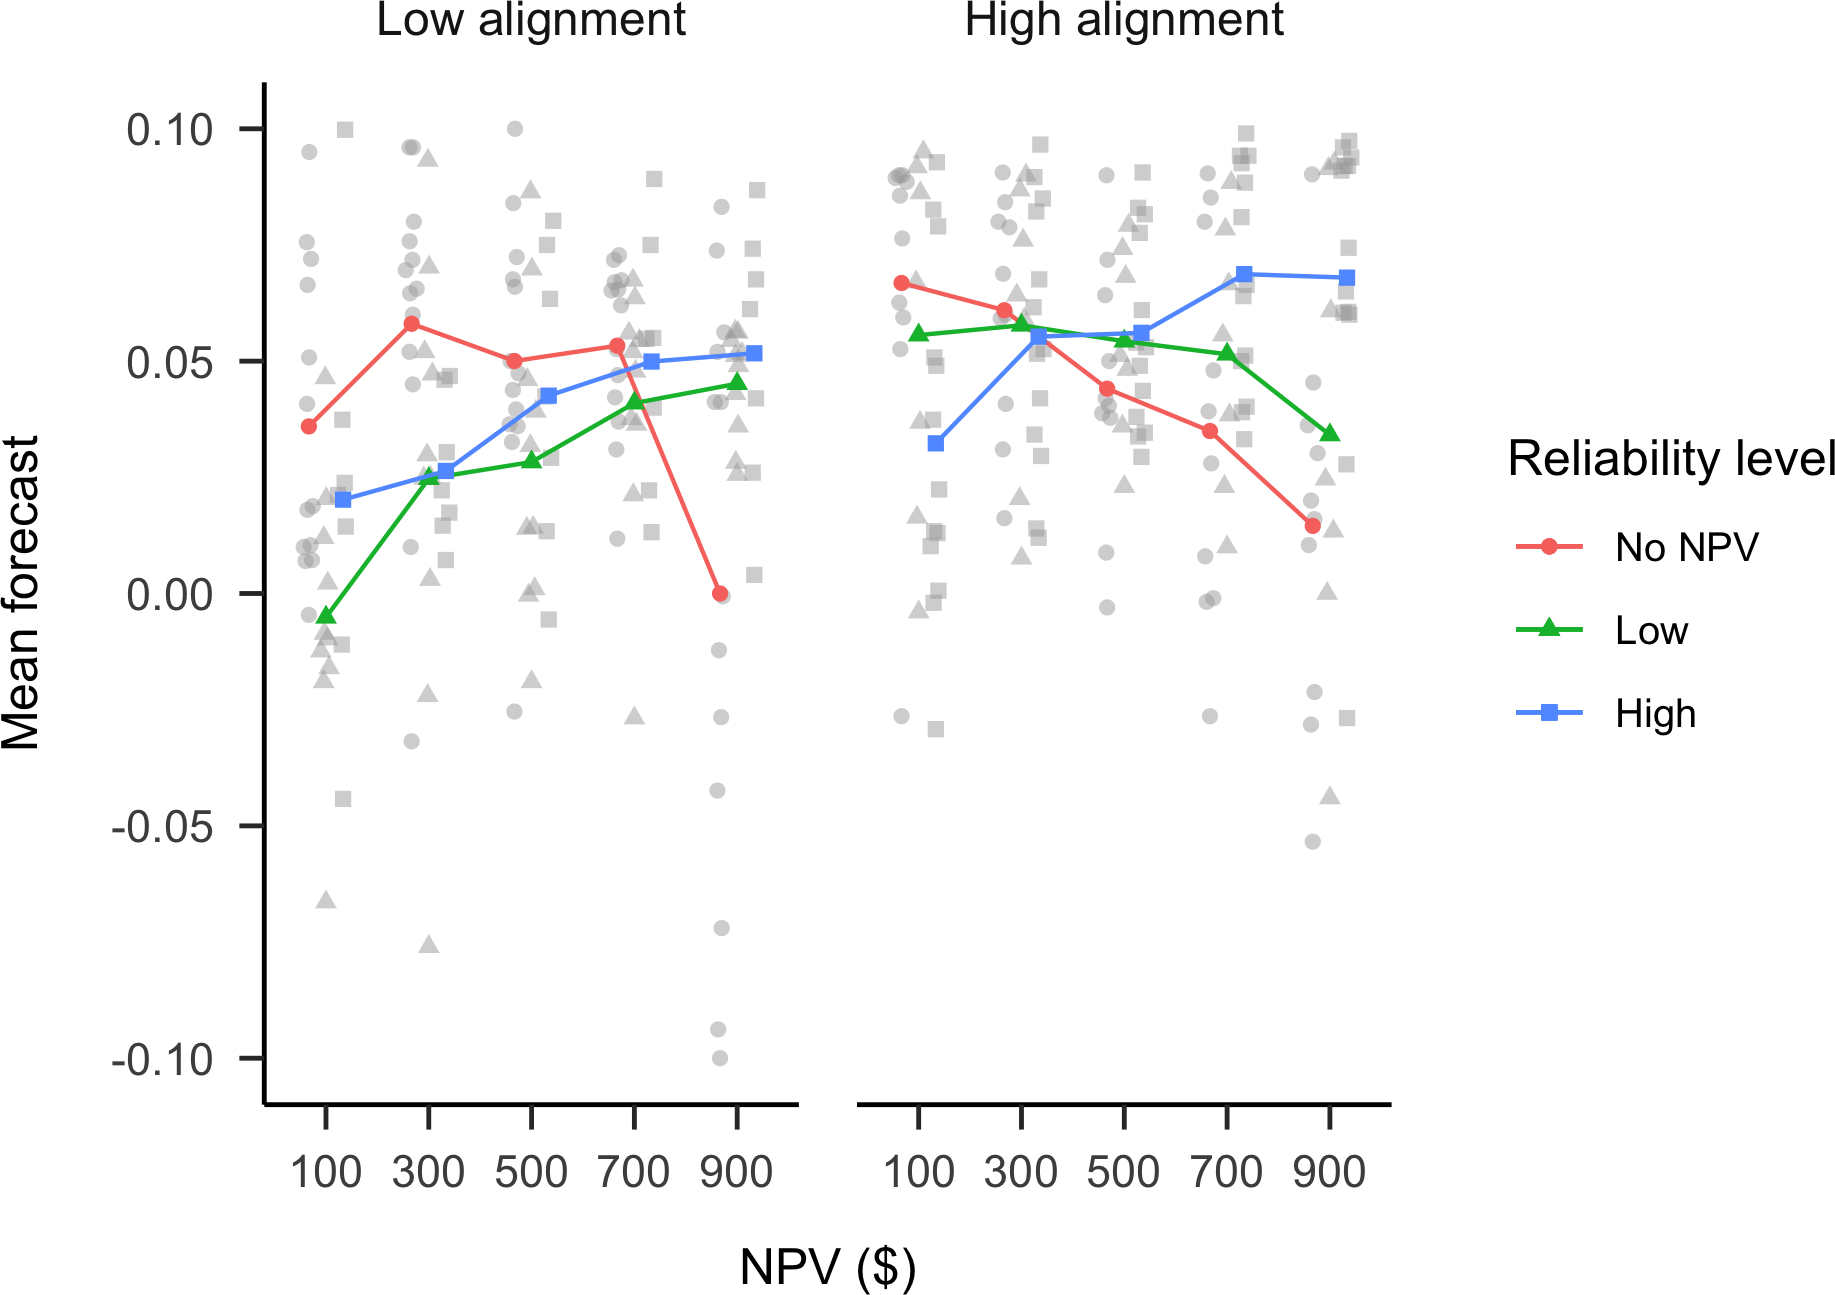
\includegraphics[width=1\linewidth]{project-similarity-bias-and-variance-neglect_files/figure-latex/plot-alignment-2-forecast-mean-1} \caption{Mean forecasts.}\label{fig:plot-alignment-2-forecast-mean}
\end{figure}

\hypertarget{forecast-sd-alignment-2}{%
\subsubsection{Forecast SD}\label{forecast-sd-alignment-2}}

A mixed factorial ANOVA was conducted to investigate the effects of alignment
and verbally-instructed NPV reliability on participants' forecast SDs. As seen
in Figure~\ref{fig:plot-alignment-2-forecast-sd}, the alignment \(\times\)
reliability level \(\times\) NPV interaction was significant,
\(F(6.87, 185.42) = 2.91\), \(p = .007\), \(\hat{\eta}^2_p = .097\).
However, none of the linear NPV trends were significantly different from each
other as above. Of relevance, the low alignment condition on average had higher
SDs than those in the high alignment condition,
\(F(1, 54) = 5.77\), \(p = .020\), \(\hat{\eta}^2_p = .097\).



\begin{figure}
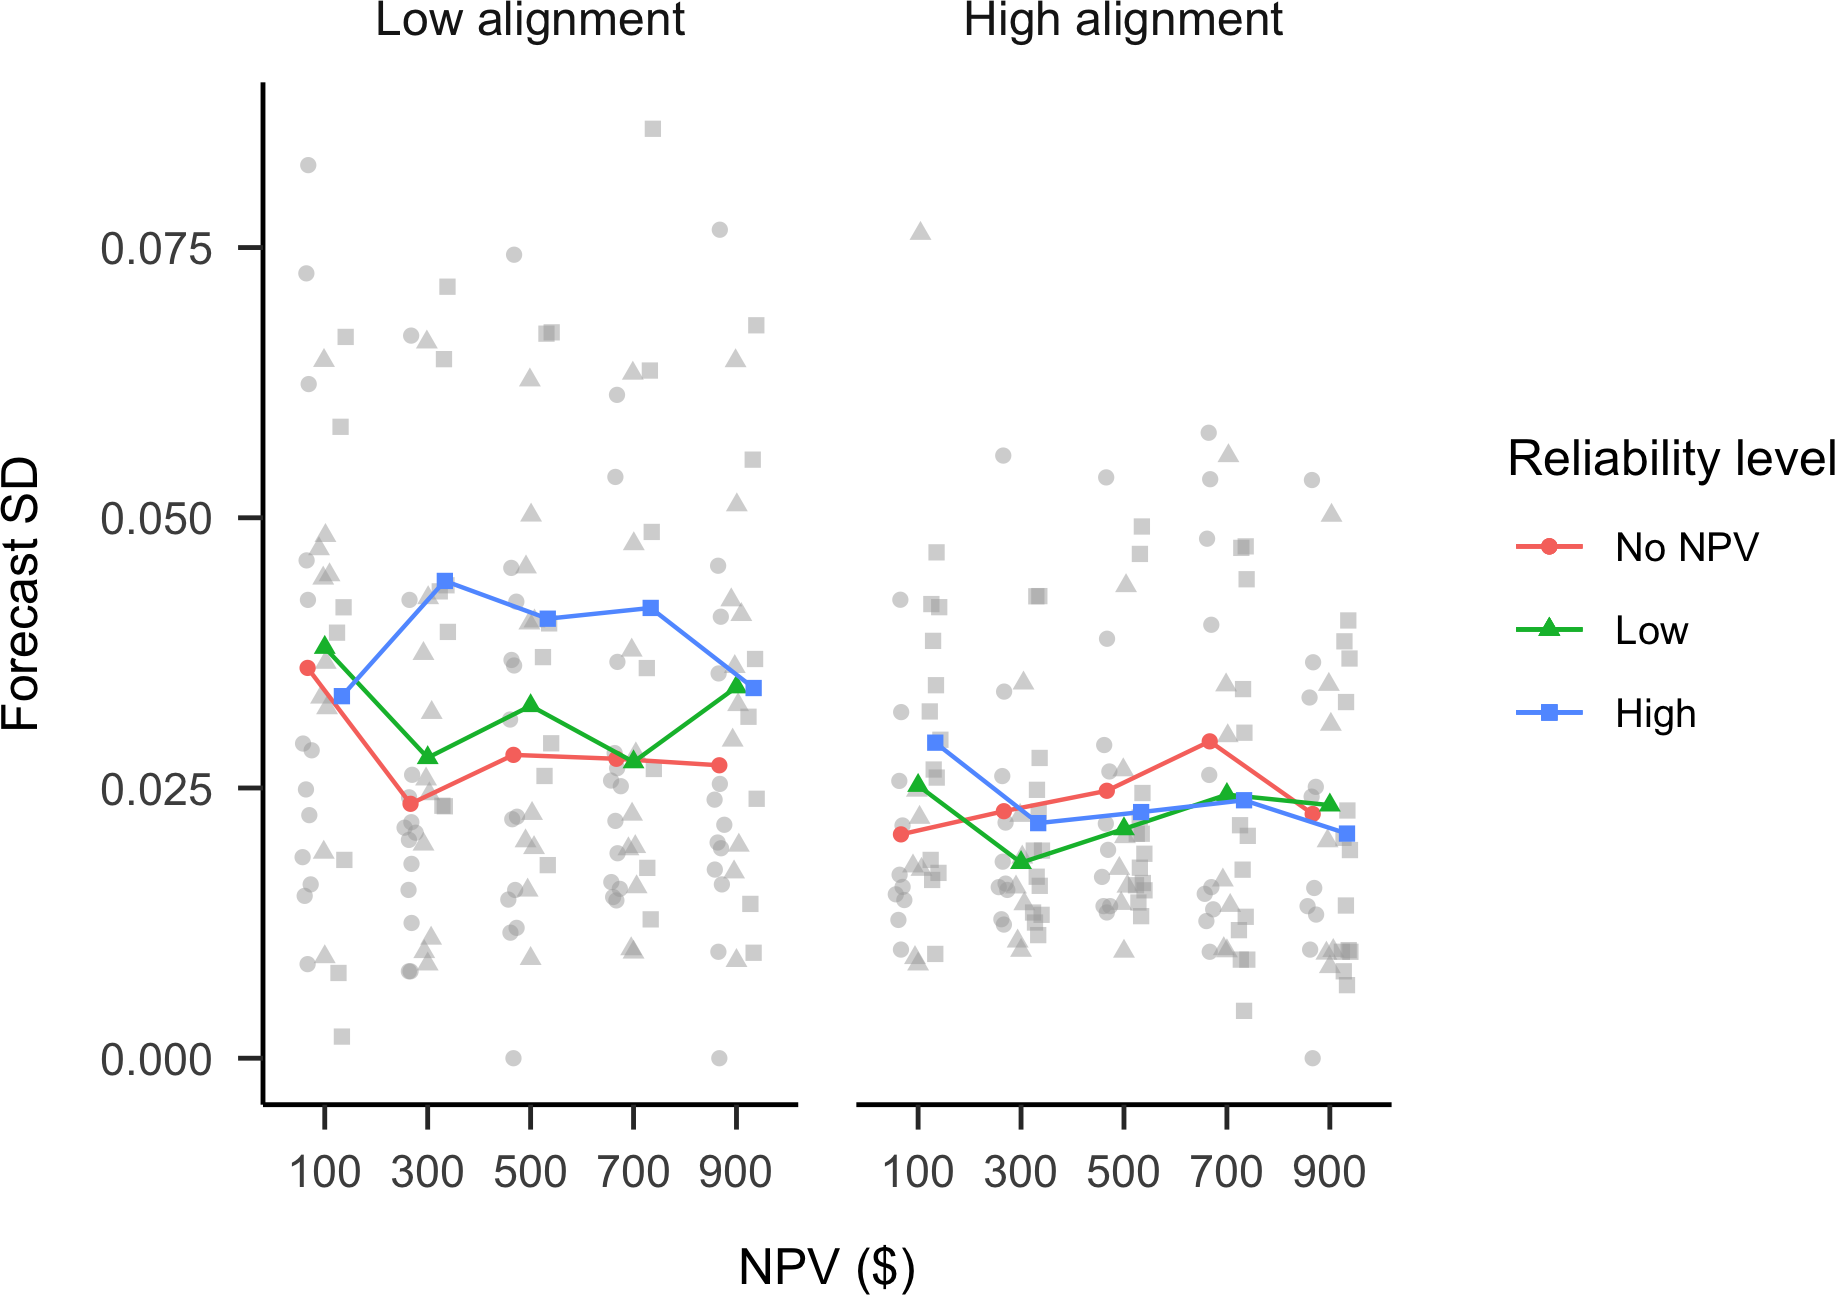
\includegraphics[width=1\linewidth]{project-similarity-bias-and-variance-neglect_files/figure-latex/plot-alignment-2-forecast-sd-1} \caption{Mean forecast SD.}\label{fig:plot-alignment-2-forecast-sd}
\end{figure}

\hypertarget{alignment-3-appendix}{%
\section{Experiment 2}\label{alignment-3-appendix}}

\hypertarget{instructions-materials-alignment-3-appendix}{%
\subsection{Instructions}\label{instructions-materials-alignment-3-appendix}}

Figure~\ref{fig:instructions-materials-alignment-3} shows the instructions.



\begin{figure}
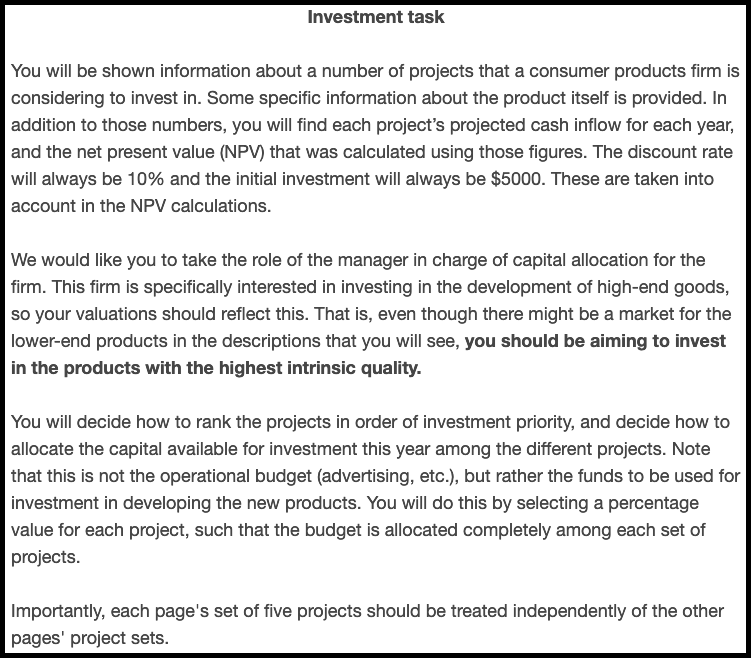
\includegraphics[width=1\linewidth]{project-similarity-bias-and-variance-neglect_files/figure-latex/instructions-materials-alignment-3-1} \caption{Experiment 2 instructions.}\label{fig:instructions-materials-alignment-3}
\end{figure}

\hypertarget{npv-test-materials-alignment-3}{%
\subsection{NPV Test}\label{npv-test-materials-alignment-3}}

Participants were given more extensive information about NPV than in the
previous experiment and were tested on their ability to calculate simple
averages from given numerical ranges, as shown in
Figures~\ref{fig:npv-test-1-materials-alignment-3}
and~\ref{fig:npv-test-2-materials-alignment-3}.



\begin{figure}
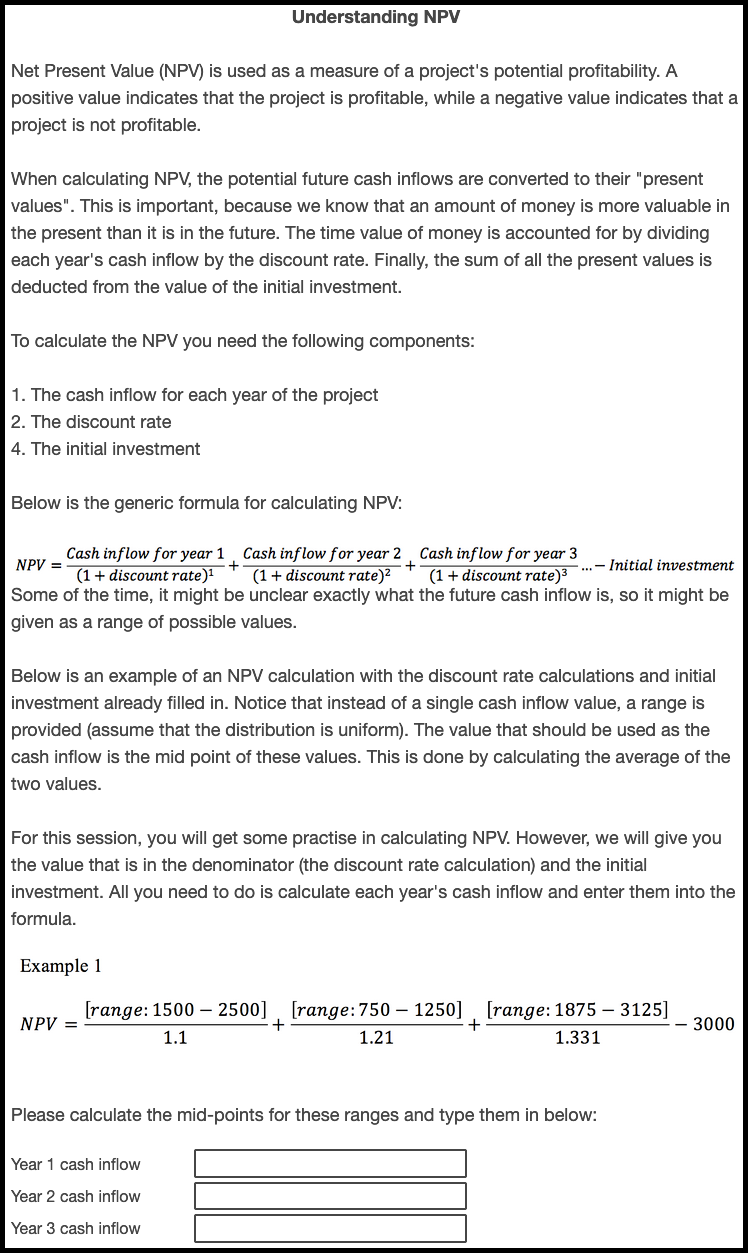
\includegraphics[width=0.9\linewidth]{project-similarity-bias-and-variance-neglect_files/figure-latex/npv-test-1-materials-alignment-3-1} \caption{Experiment 2 NPV test.}\label{fig:npv-test-1-materials-alignment-3}
\end{figure}



\begin{figure}
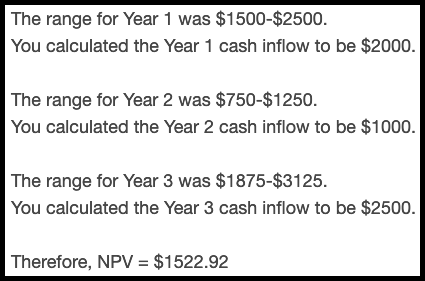
\includegraphics[width=0.6\linewidth]{project-similarity-bias-and-variance-neglect_files/figure-latex/npv-test-2-materials-alignment-3-1} \caption{Experiment 2 NPV test answers.}\label{fig:npv-test-2-materials-alignment-3}
\end{figure}

\hypertarget{npv-knowledge-materials-alignment-3}{%
\subsection{NPV Knowledge Ratings}\label{npv-knowledge-materials-alignment-3}}

A similar design to Long et al. (\protect\hyperlink{ref-long2018}{2018} Study~1) was used to test whether this sample may
be overconfident in their understanding on NPV. Therefore, participants were
asked to rate their knowledge of NPV in various points in the study.
Figure~\ref{fig:npv-knowledge-materials-alignment-3} shows an example of one
such display.



\begin{figure}
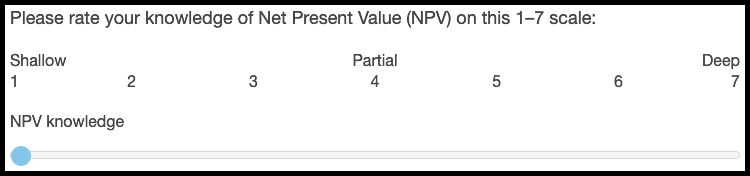
\includegraphics[width=1\linewidth]{project-similarity-bias-and-variance-neglect_files/figure-latex/npv-knowledge-materials-alignment-3-1} \caption{Experiment 2 NPV knowledge rating task.}\label{fig:npv-knowledge-materials-alignment-3}
\end{figure}

\newpage
\newpage

\hypertarget{variance-lecture-materials-alignment-3}{%
\subsection{Variance Lecture}\label{variance-lecture-materials-alignment-3}}

See below the slides for the variance lecture.

\begin{figure} \makebox[\linewidth][c]{\fbox{\includegraphics[width=1.2\linewidth]{/Users/shirdekel/Library/Application Support/renv/cache/v5/R-4.0/x86_64-apple-darwin17.0/alignment3/1.0/b278410953893fa36e2151055fbbe2dc/alignment3/materials/variance_lecture_split//_00000000000001.pdf}}} \caption{Variance lecture slide 1.} \end{figure}
 \begin{figure} \makebox[\linewidth][c]{\fbox{\includegraphics[width=1.2\linewidth]{/Users/shirdekel/Library/Application Support/renv/cache/v5/R-4.0/x86_64-apple-darwin17.0/alignment3/1.0/b278410953893fa36e2151055fbbe2dc/alignment3/materials/variance_lecture_split//_00000000000002.pdf}}} \caption{Variance lecture slide 2.} \end{figure}
 \begin{figure} \makebox[\linewidth][c]{\fbox{\includegraphics[width=1.2\linewidth]{/Users/shirdekel/Library/Application Support/renv/cache/v5/R-4.0/x86_64-apple-darwin17.0/alignment3/1.0/b278410953893fa36e2151055fbbe2dc/alignment3/materials/variance_lecture_split//_00000000000003.pdf}}} \caption{Variance lecture slide 3.} \end{figure}
 \begin{figure} \makebox[\linewidth][c]{\fbox{\includegraphics[width=1.2\linewidth]{/Users/shirdekel/Library/Application Support/renv/cache/v5/R-4.0/x86_64-apple-darwin17.0/alignment3/1.0/b278410953893fa36e2151055fbbe2dc/alignment3/materials/variance_lecture_split//_00000000000004.pdf}}} \caption{Variance lecture slide 4.} \end{figure}
 \begin{figure} \makebox[\linewidth][c]{\fbox{\includegraphics[width=1.2\linewidth]{/Users/shirdekel/Library/Application Support/renv/cache/v5/R-4.0/x86_64-apple-darwin17.0/alignment3/1.0/b278410953893fa36e2151055fbbe2dc/alignment3/materials/variance_lecture_split//_00000000000005.pdf}}} \caption{Variance lecture slide 5.} \end{figure}
 \begin{figure} \makebox[\linewidth][c]{\fbox{\includegraphics[width=1.2\linewidth]{/Users/shirdekel/Library/Application Support/renv/cache/v5/R-4.0/x86_64-apple-darwin17.0/alignment3/1.0/b278410953893fa36e2151055fbbe2dc/alignment3/materials/variance_lecture_split//_00000000000006.pdf}}} \caption{Variance lecture slide 6.} \end{figure}
 \begin{figure} \makebox[\linewidth][c]{\fbox{\includegraphics[width=1.2\linewidth]{/Users/shirdekel/Library/Application Support/renv/cache/v5/R-4.0/x86_64-apple-darwin17.0/alignment3/1.0/b278410953893fa36e2151055fbbe2dc/alignment3/materials/variance_lecture_split//_00000000000007.pdf}}} \caption{Variance lecture slide 7.} \end{figure}
 \begin{figure} \makebox[\linewidth][c]{\fbox{\includegraphics[width=1.2\linewidth]{/Users/shirdekel/Library/Application Support/renv/cache/v5/R-4.0/x86_64-apple-darwin17.0/alignment3/1.0/b278410953893fa36e2151055fbbe2dc/alignment3/materials/variance_lecture_split//_00000000000008.pdf}}} \caption{Variance lecture slide 8.} \end{figure}
 \begin{figure} \makebox[\linewidth][c]{\fbox{\includegraphics[width=1.2\linewidth]{/Users/shirdekel/Library/Application Support/renv/cache/v5/R-4.0/x86_64-apple-darwin17.0/alignment3/1.0/b278410953893fa36e2151055fbbe2dc/alignment3/materials/variance_lecture_split//_00000000000009.pdf}}} \caption{Variance lecture slide 9.} \end{figure}
 \begin{figure} \makebox[\linewidth][c]{\fbox{\includegraphics[width=1.2\linewidth]{/Users/shirdekel/Library/Application Support/renv/cache/v5/R-4.0/x86_64-apple-darwin17.0/alignment3/1.0/b278410953893fa36e2151055fbbe2dc/alignment3/materials/variance_lecture_split//_00000000000010.pdf}}} \caption{Variance lecture slide 10.} \end{figure}
 \begin{figure} \makebox[\linewidth][c]{\fbox{\includegraphics[width=1.2\linewidth]{/Users/shirdekel/Library/Application Support/renv/cache/v5/R-4.0/x86_64-apple-darwin17.0/alignment3/1.0/b278410953893fa36e2151055fbbe2dc/alignment3/materials/variance_lecture_split//_00000000000011.pdf}}} \caption{Variance lecture slide 11.} \end{figure}
 \begin{figure} \makebox[\linewidth][c]{\fbox{\includegraphics[width=1.2\linewidth]{/Users/shirdekel/Library/Application Support/renv/cache/v5/R-4.0/x86_64-apple-darwin17.0/alignment3/1.0/b278410953893fa36e2151055fbbe2dc/alignment3/materials/variance_lecture_split//_00000000000012.pdf}}} \caption{Variance lecture slide 12.} \end{figure}
 \begin{figure} \makebox[\linewidth][c]{\fbox{\includegraphics[width=1.2\linewidth]{/Users/shirdekel/Library/Application Support/renv/cache/v5/R-4.0/x86_64-apple-darwin17.0/alignment3/1.0/b278410953893fa36e2151055fbbe2dc/alignment3/materials/variance_lecture_split//_00000000000013.pdf}}} \caption{Variance lecture slide 13.} \end{figure}
 \begin{figure} \makebox[\linewidth][c]{\fbox{\includegraphics[width=1.2\linewidth]{/Users/shirdekel/Library/Application Support/renv/cache/v5/R-4.0/x86_64-apple-darwin17.0/alignment3/1.0/b278410953893fa36e2151055fbbe2dc/alignment3/materials/variance_lecture_split//_00000000000014.pdf}}} \caption{Variance lecture slide 14.} \end{figure}

\hypertarget{results-alignment-3-appendix}{%
\subsection{Additional Analyses}\label{results-alignment-3-appendix}}

\hypertarget{ranking-1}{%
\subsubsection{Ranking}\label{ranking-1}}

A mixed factorial ANOVA was conducted to investigate the effects of NPV,
alignment, and numerical NPV reliability on participants' project rankings.
Figure~\ref{fig:plot-alignment-3-ranking} shows these data. The alignment
\(\times\) reliability level \(\times\) NPV interaction was not
significant,
\(F(3.00, 159.10) = 2.44\), \(p = .066\), \(\hat{\eta}^2_p = .044\).
However, the alignment \(\times\) NPV interaction was significant,
\(F(1.99, 105.72) = 16.97\), \(p < .001\), \(\hat{\eta}^2_p = .243\); as well as the reliability
amount \(\times\) NPV interaction,
\(F(3.28, 173.93) = 2.67\), \(p = .044\), \(\hat{\eta}^2_p = .048\). As in the
allocation data, the linear NPV trend did not differ between reliability level
condition in neither the low alignment condition,
\(\Delta M = 0.43\), 95\% CI \([-0.77, 1.63]\), \(t(53) = 0.71\), \(p = .480\), nor the high alignment
condition, \(\Delta M = 0.46\), 95\% CI \([-0.92, 1.84]\), \(t(53) = 0.67\), \(p = .504\). However,
averaging over reliability level, the linear NPV trend was higher in the low
alignment condition than in the high alignment condition,
\(\Delta M = -4.54\), 95\% CI \([-6.39, -2.68]\), \(t(53) = -4.91\), \(p < .001\).



\begin{figure}
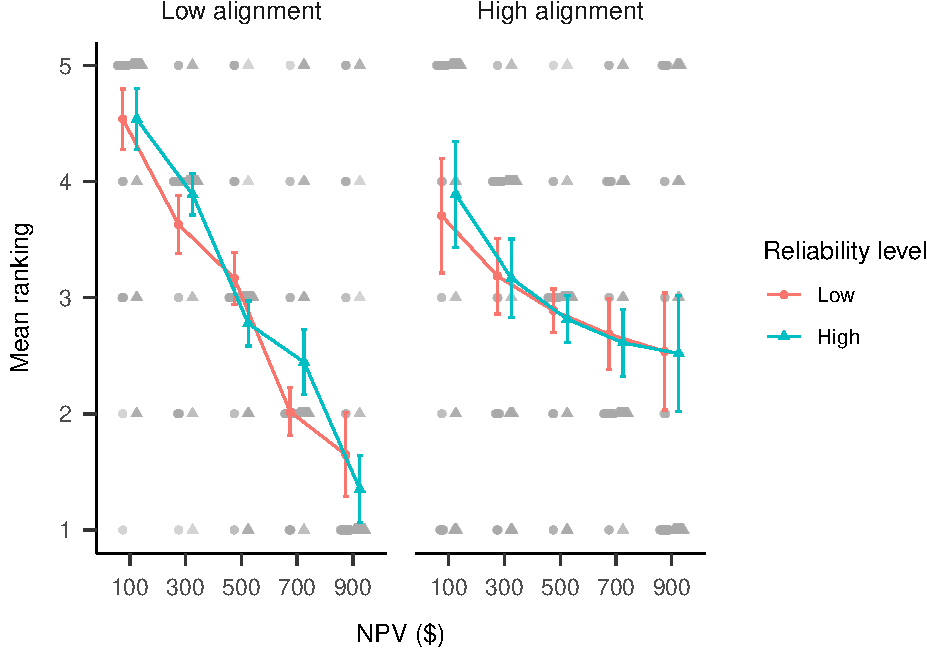
\includegraphics[width=1\linewidth]{project-similarity-bias-and-variance-neglect_files/figure-latex/plot-alignment-3-ranking-1} \caption{Mean ranking.}\label{fig:plot-alignment-3-ranking}
\end{figure}

\hypertarget{confidence-1}{%
\subsubsection{Confidence}\label{confidence-1}}

A mixed factorial ANOVA was conducted to investigate the effects of NPV,
alignment, and numerical NPV reliability on participants' confidence ratings.
Figure~\ref{fig:plot-alignment-3-confidence} shows these data. Only the main
effect of NPV was significant,
\(F(2.62, 139.08) = 2.97\), \(p = .041\), \(\hat{\eta}^2_p = .053\).



\begin{figure}
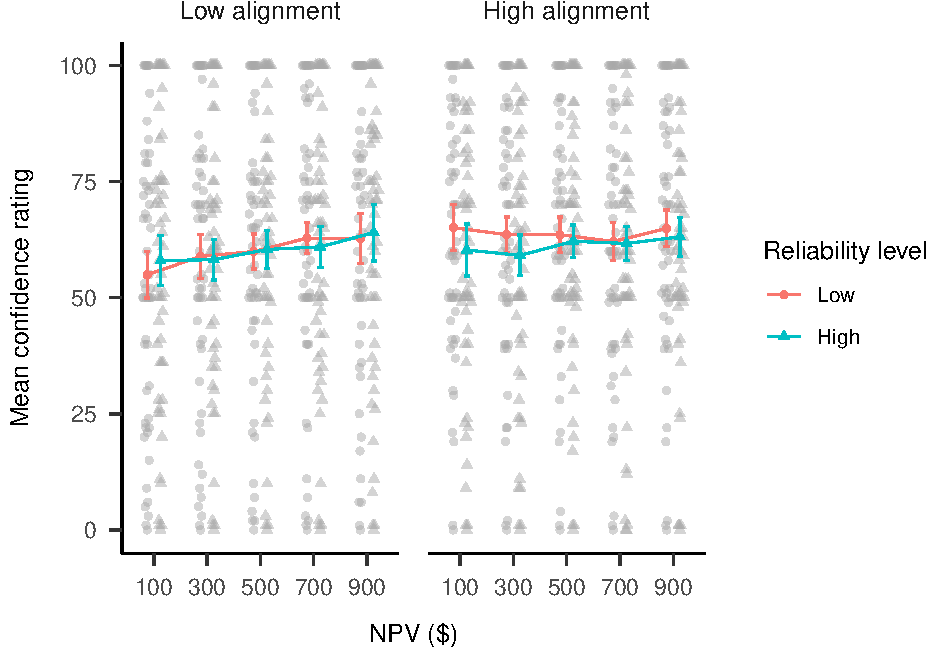
\includegraphics[width=1\linewidth]{project-similarity-bias-and-variance-neglect_files/figure-latex/plot-alignment-3-confidence-1} \caption{Mean confidence.}\label{fig:plot-alignment-3-confidence}
\end{figure}

\hypertarget{variance-lecture-1}{%
\subsubsection{Variance Lecture}\label{variance-lecture-1}}

The allocation and ranking data show that participants were affected by the
similarity of options, but were not affected by variance information. After the
main task of this experiment, participants were shown a short lecture about the
importance of variance information when making allocation decisions. They were
then presented with half of their previous allocations and gave them an
opportunity to amend their allocations. It was hypothesised that participants
will be more sensitive to variance after the educational intervention.

A mixed factorial ANOVA was conducted to investigate the effects of phase on
participants' project allocations. As shown in
Figure~\ref{fig:plot-alignment-3-variance-lecture}, the four-way interaction
was not significant,
\(F(2.56, 133.09) = 1.74\), \(p = .169\), \(\hat{\eta}^2_p = .032\).
Further, the NPV \(\times\) phase \(\times\) reliability level interactions were not
significant for either the low alignment condition,
\(\Delta M = 4.43\), 95\% CI \([-23.71, 32.58]\), \(t(52) = 0.32\), \(p = .753\); or the
high alignment conditions,
\(\Delta M = -11.92\), 95\% CI \([-43.39, 19.55]\), \(t(52) = -0.76\), \(p = .451\). In the
low alignment condition, the linear NPV trend (averaged over reliability level)
was significantly weaker after the lecture, compared with the linear NPV trend
before the lecture, \(\Delta M = -12.85\), 95\% CI \([-24.08, -1.62]\), \(t(52) = -2.30\), \(p = .026\).
However, this comparison was not significant in the high alignment condition,
\(\Delta M = -6.37\), 95\% CI \([-18.93, 6.18]\), \(t(52) = -1.02\), \(p = .313\). These results
suggest that participants did not become better informed by NPV numerical
reliability after the variance lecture. There was, however, some reduction in
reliance on NPV overall when projects were dissimilar.



\begin{figure}[!htbp]
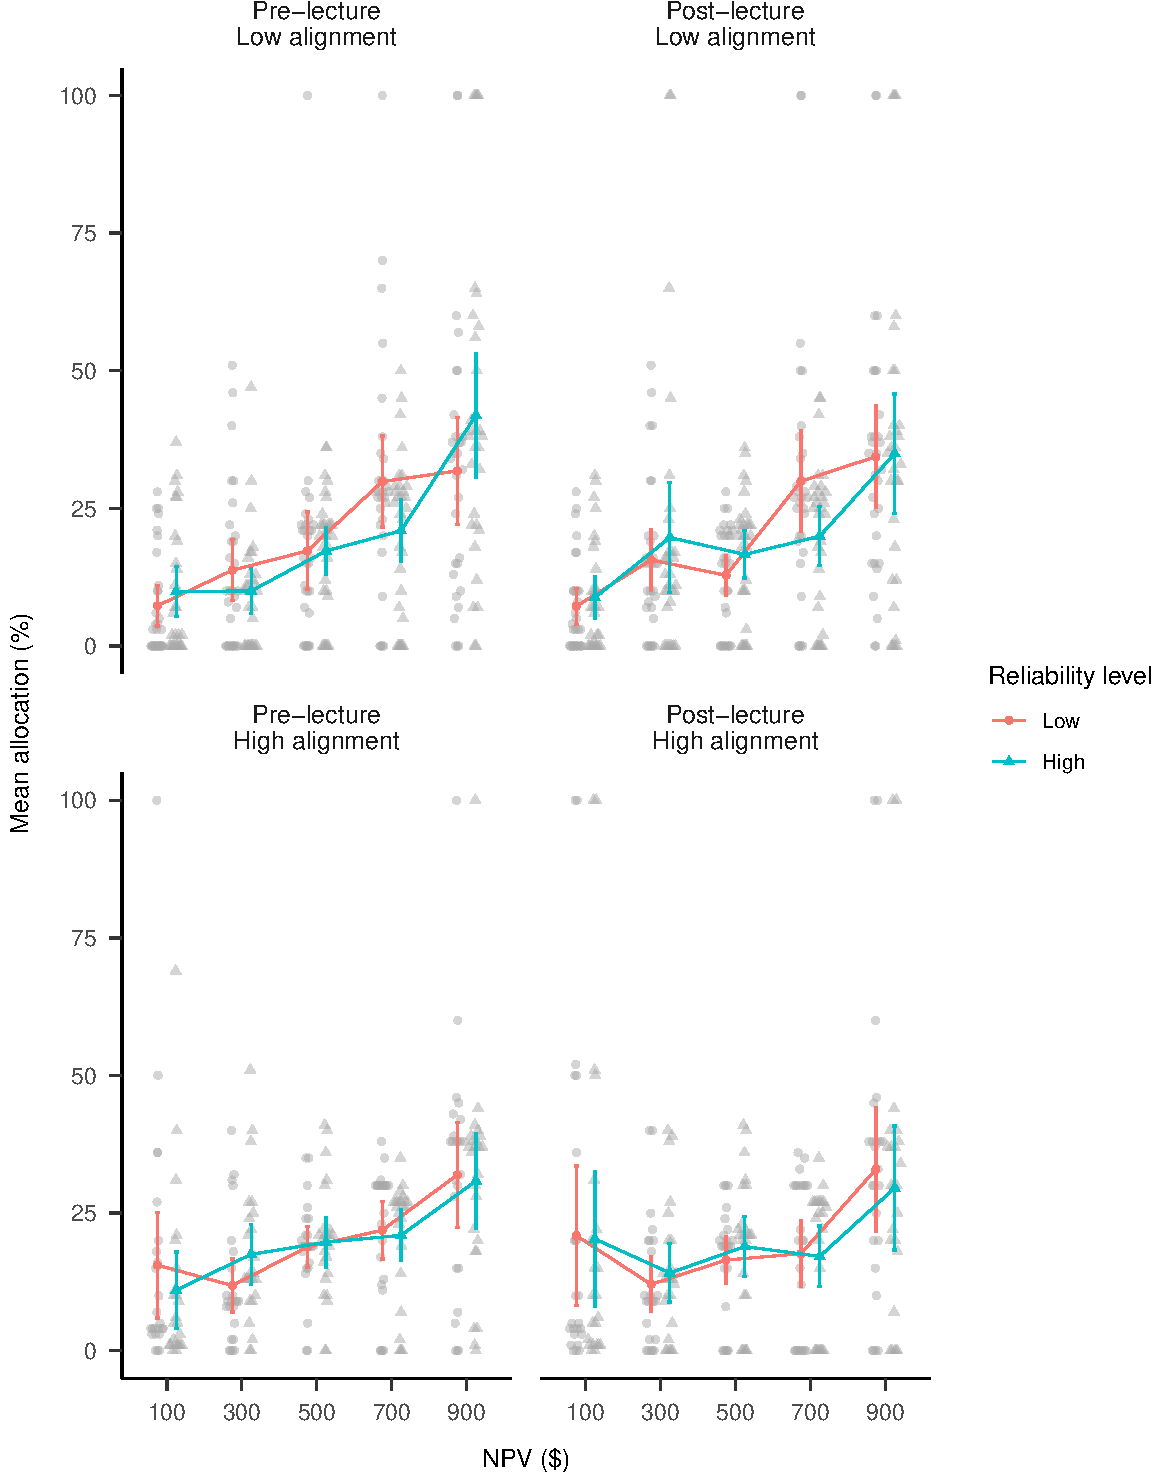
\includegraphics[width=1\linewidth]{project-similarity-bias-and-variance-neglect_files/figure-latex/plot-alignment-3-variance-lecture-1} \caption{Mean allocation by NPV, reliability level, alignment, and phase.}\label{fig:plot-alignment-3-variance-lecture}
\end{figure}

\hypertarget{npv-knowledge}{%
\subsubsection{NPV Knowledge}\label{npv-knowledge}}

A repeated-measures ANOVA was conducted to investigate the effects of experiment
phase condition on participants' NPV knowledge rating.
Figure~\ref{fig:plot-alignment-3-npv-knowledge} shows these data. The main
effect of phase was significant, \(F(2.43, 128.59) = 7.80\), \(p < .001\), \(\hat{\eta}^2_p = .128\).
The post-explanation rating was significantly higher than the pre-explanation
rating,
\(\Delta M = -0.59\), \(95\%\ \mathrm{CI}_\mathrm{\scriptsize Tukey(5)}\) \([-0.92, -0.26]\), \(t(53) = -5.07\), \(p_\mathrm{\scriptsize Tukey(5)} < .001\). However, there were no significant
differences in rating between any of the later phases.



\begin{figure}
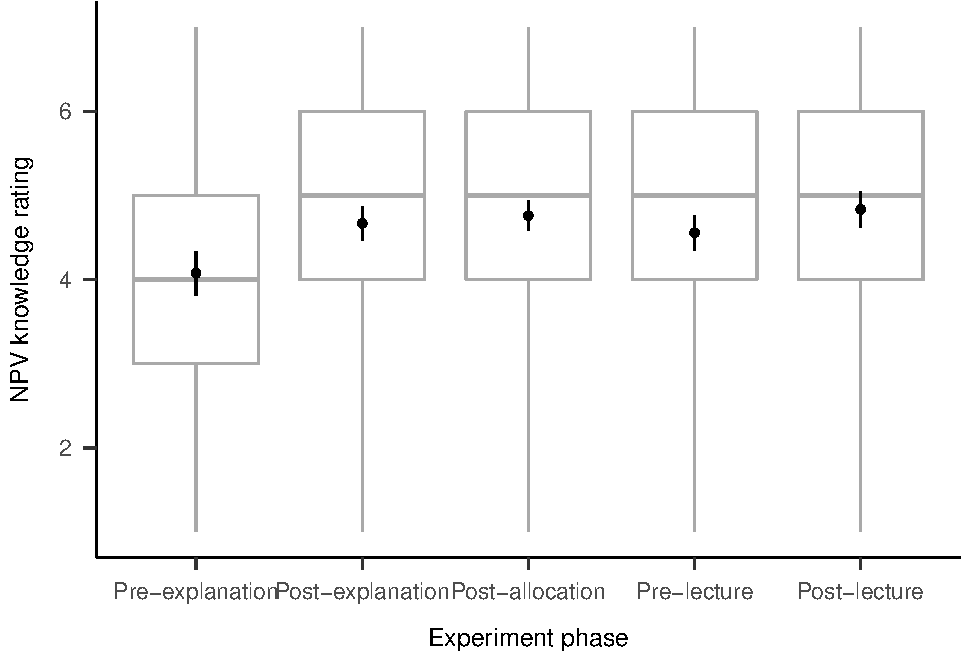
\includegraphics[width=1\linewidth]{project-similarity-bias-and-variance-neglect_files/figure-latex/plot-alignment-3-npv-knowledge-1} \caption{Mean NPV knowledge rating.}\label{fig:plot-alignment-3-npv-knowledge}
\end{figure}

\hypertarget{experiment-3}{%
\section{Experiment~3}\label{experiment-3}}

\hypertarget{alignment-8-appendix}{%
\subsection{Hypothesised Effects}\label{alignment-8-appendix}}

Figure~\ref{fig:plot-simulation-alignment-8} shows the simulated hypothesised
effects for Experiment~3. These effects were constructed as a composite of
Experiment~1 data (without the no NPV condition) for the verbal reliability type
condition, and data from a pilot study (Dekel, \protect\hyperlink{ref-dekel2021b}{2021}, Appendix B.8) for the
numerical reliability type condition. Variance was removed to see the effects
clearer.



\begin{figure}
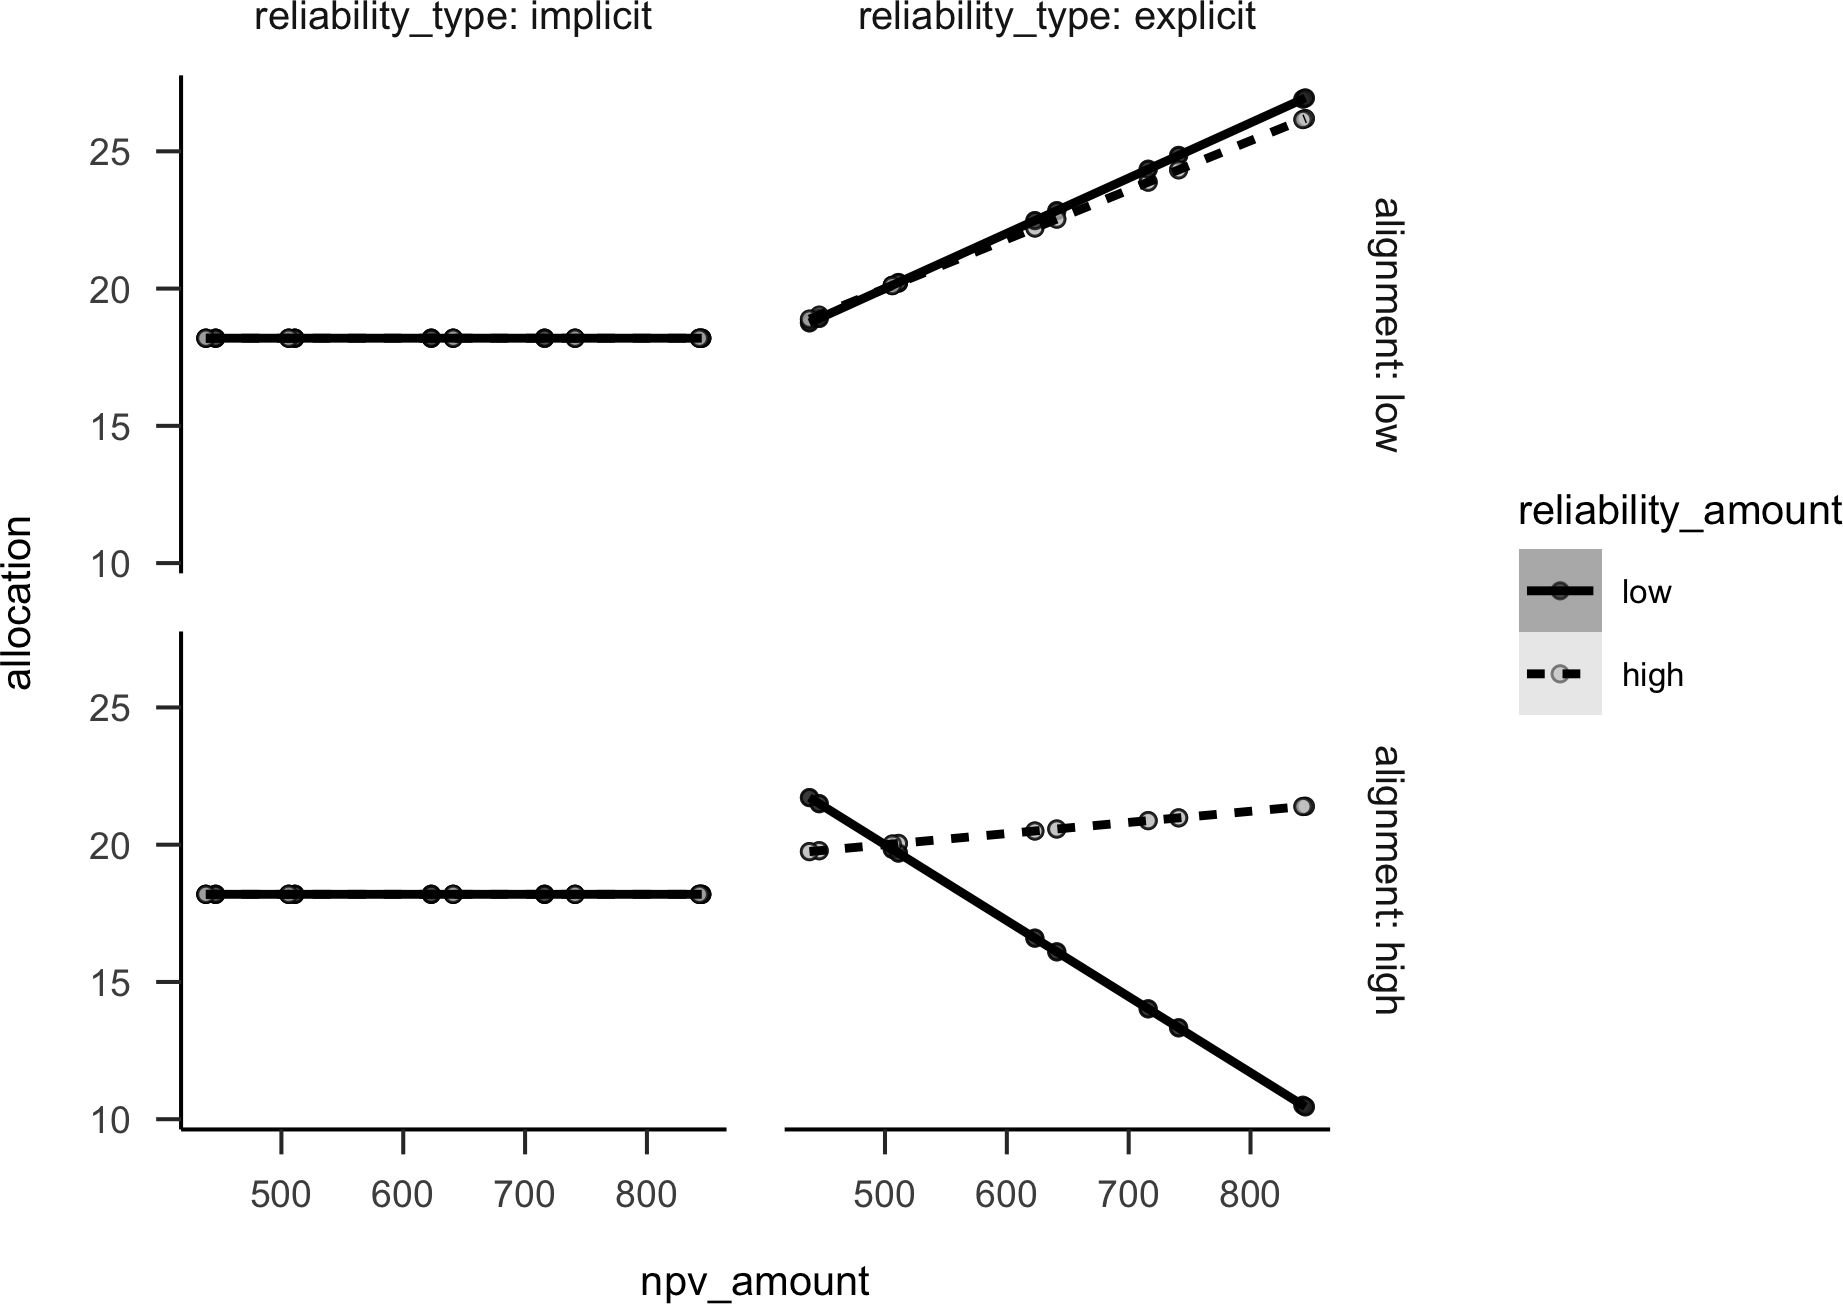
\includegraphics[width=1\linewidth]{project-similarity-bias-and-variance-neglect_files/figure-latex/plot-simulation-alignment-8-1} \caption{Experiment~3 predicted data.}\label{fig:plot-simulation-alignment-8}
\end{figure}

\hypertarget{power-analysis-alignment-8}{%
\subsection{Power Analysis}\label{power-analysis-alignment-8}}

A power analysis was conducted through simulation of the effects hypothesised in
Experiment~3 (and the simple effects implied by them). The simulated data used
the same regression coefficients as Experiment~2 for the explicit condition, no
effects for the implicit condition (as shown in
Figure~\ref{fig:plot-simulation-alignment-8}), and the intercept and residual
variance of Experiment~2. The null effects were analysed using the two one-sided
tests (TOST) procedure, or \emph{equivalence} testing (Lakens et al., \protect\hyperlink{ref-lakens2018}{2018}), and setting the
smallest effect size of interest to the smallest difference that leads to a
significant equivalence between low and high implicit reliability for low
alignment in a pilot study (Dekel, \protect\hyperlink{ref-dekel2021b}{2021}, Appendix B.8).
Figure~\ref{fig:power-curve-alignment-8} shows the resulting power curve. The
analysis suggests a total sample size of 448
(112 \(\cdot\) 4).

\newpage

\begin{landscape}



\begin{figure}
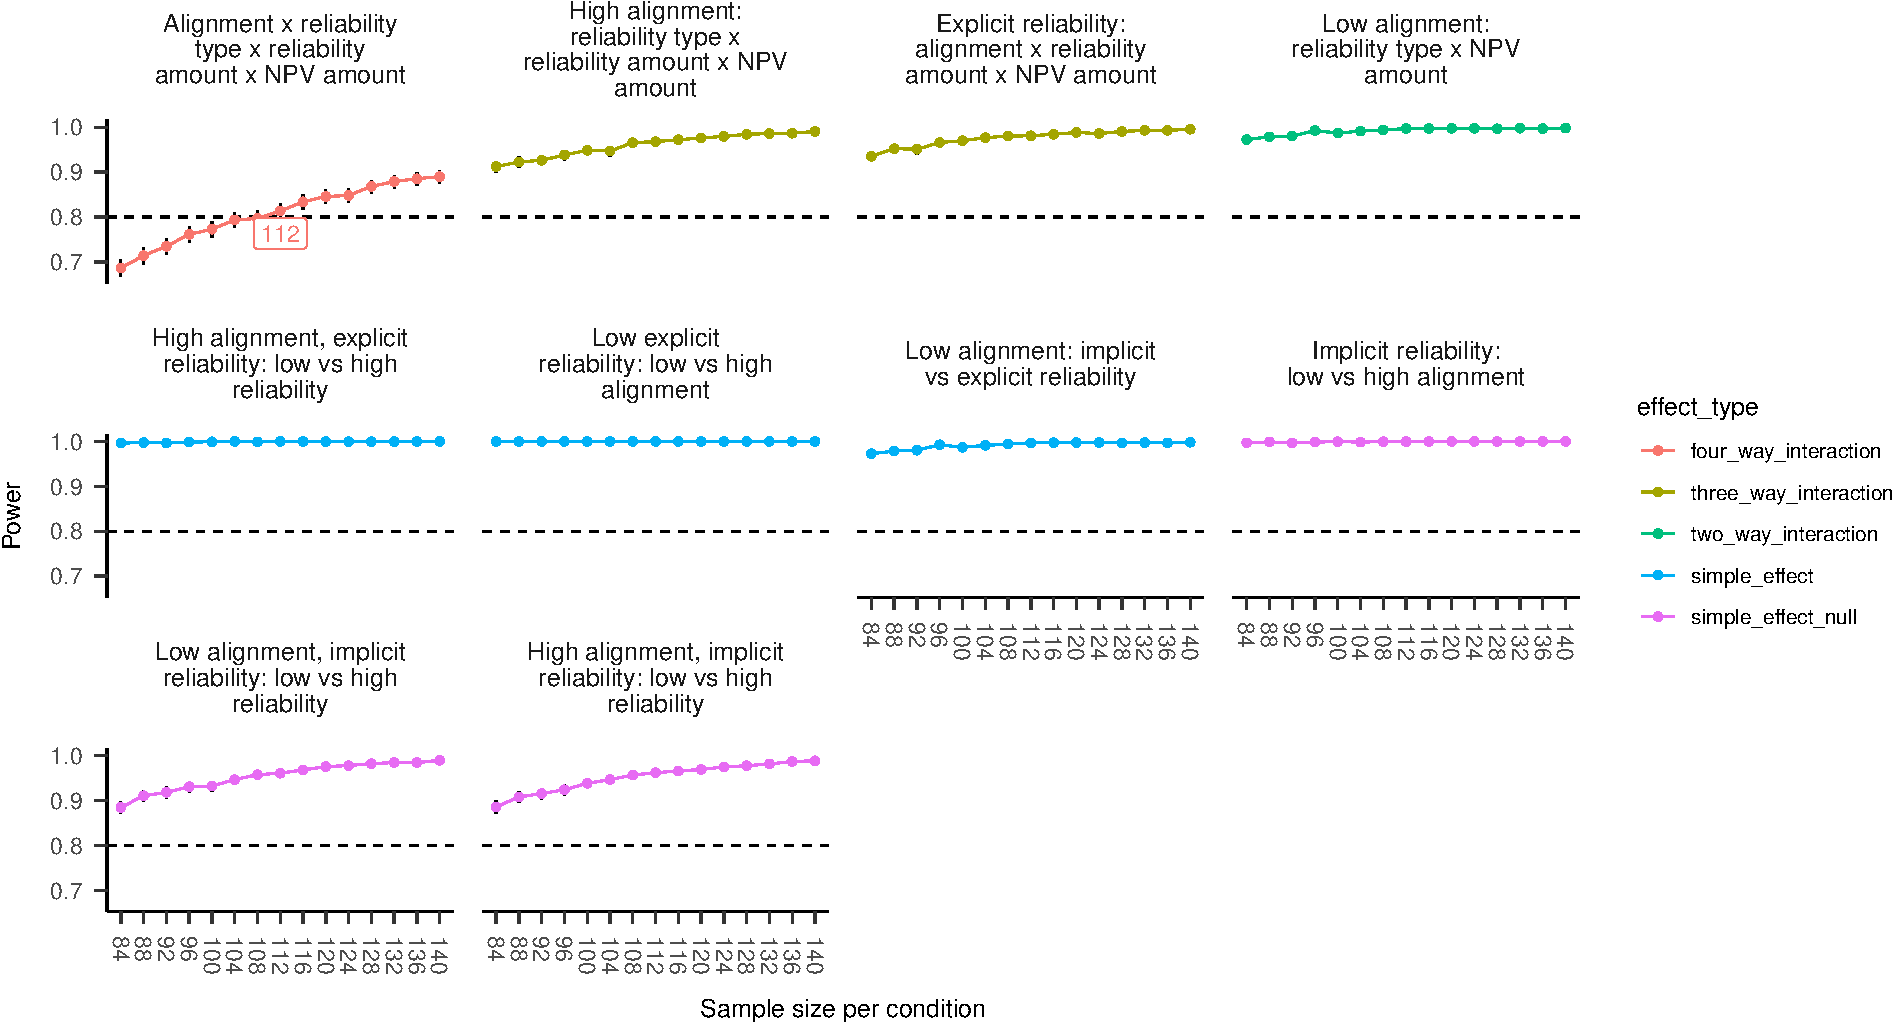
\includegraphics[width=1\linewidth]{project-similarity-bias-and-variance-neglect_files/figure-latex/power-curve-alignment-8-1} \caption{Alignment Experiment~3 power curve. Labels indicate lowest sample size above 80\% power.}\label{fig:power-curve-alignment-8}
\end{figure}

\end{landscape}

\newpage

\hypertarget{instructions-materials-alignment-8-appendix}{%
\subsection{Instructions}\label{instructions-materials-alignment-8-appendix}}

Figures~\ref{fig:instructions-reliability-explicit-materials-alignment-8}
and~\ref{fig:instructions-reliability-implicit-materials-alignment-8} show the
instructions for the verbal and numerical reliability conditions, respectively.



\begin{figure}
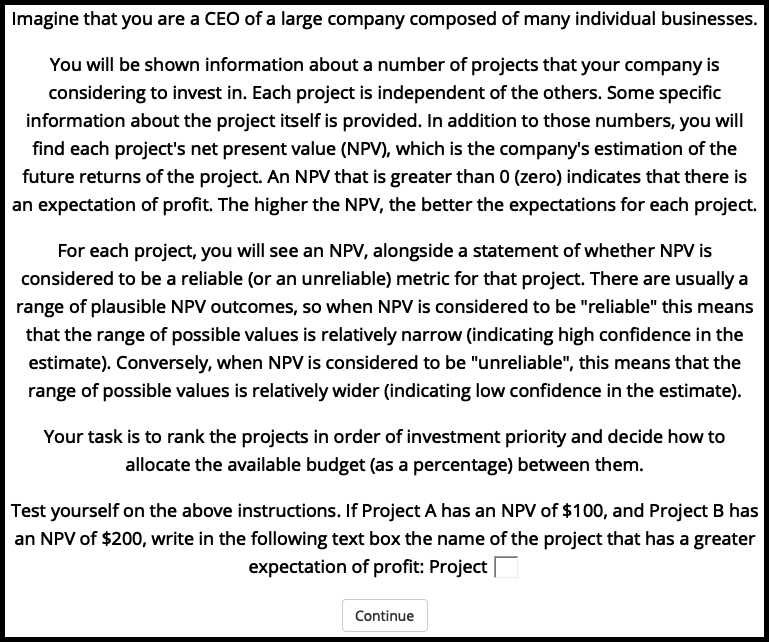
\includegraphics[width=1\linewidth]{project-similarity-bias-and-variance-neglect_files/figure-latex/instructions-reliability-explicit-materials-alignment-8-1} \caption{Experiment~3 verbal reliability instructions.}\label{fig:instructions-reliability-explicit-materials-alignment-8}
\end{figure}



\begin{figure}
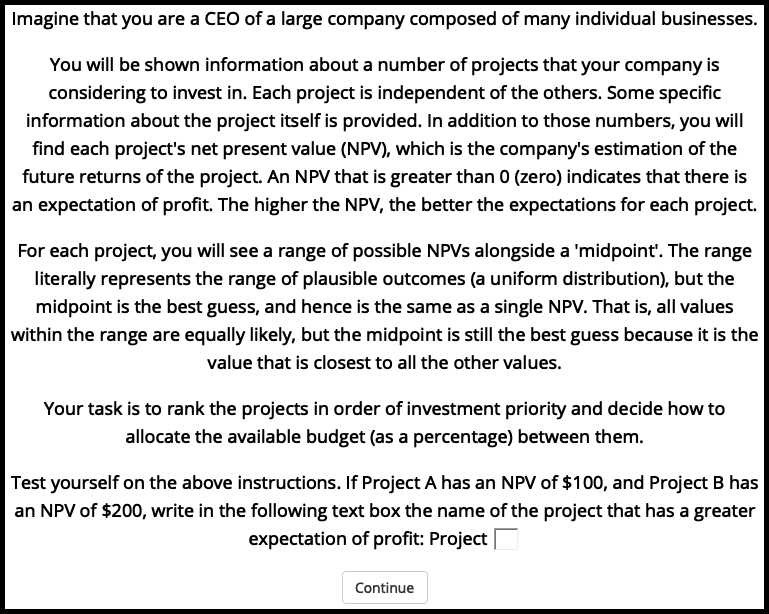
\includegraphics[width=1\linewidth]{project-similarity-bias-and-variance-neglect_files/figure-latex/instructions-reliability-implicit-materials-alignment-8-1} \caption{Experiment~3 numerical reliability instructions.}\label{fig:instructions-reliability-implicit-materials-alignment-8}
\end{figure}

\hypertarget{interstitial-materials-alignment-8}{%
\subsection{Interstitial Display}\label{interstitial-materials-alignment-8}}

Figure~\ref{fig:interstitial-materials-alignment-8} shows an example of an
interstitial display.



\begin{figure}

\includegraphics[width=1\linewidth]{project-similarity-bias-and-variance-neglect_files/figure-latex/interstitial-materials-alignment-8-1} \caption{An example of an interstitial display in Experiment~3.}\label{fig:interstitial-materials-alignment-8}
\end{figure}

\hypertarget{results-alignment-8-allocation}{%
\subsection{Additional Analyses}\label{results-alignment-8-allocation}}

The three-way interaction (reliability level \(\times\) NPV \(\times\) reliability
type) in the high alignment condition was significant,
\(\Delta M = 35.43\), 95\% CI \([20.74, 50.12]\), \(t(444) = 4.74\), \(p < .001\). The NPV \(\times\)
reliability type (averaging over reliability level) in the low alignment
condition was significant,
\(\Delta M = 11.48\), 95\% CI \([0.19, 22.77]\), \(t(444) = 2.00\), \(p = .046\). The association
between allocation and NPV for those in the explicit low reliability
condition was significantly stronger for those in the low alignment condition,
than for those in the high alignment condition,
\(\Delta M = 35.68\), 95\% CI \([22.27, 49.09]\), \(t(444) = 5.23\), \(p < .001\).
The linear NPV trend for those in the low alignment condition was
significantly stronger for those in the explicit reliability condition, than for
those in the implicit reliability condition (averaging over reliability level),
\(\Delta M = 11.48\), 95\% CI \([0.19, 22.77]\), \(t(444) = 2.00\), \(p = .046\). The linear
NPV trend for those in the implicit reliability condition was not
significantly ``equivalent'' between those in the low and high reliability
conditions for both those in the low alignment
\(\Delta M = 1.64\), 95\% CI \([-8.74, 12.03]\), \(t(444) = 0.31\), \(p = .620\)
and high alignment conditions
\(\Delta M = -1.21\), 95\% CI \([-11.59, 9.18]\), \(t(444) = 0.22\), \(p = .589\).
However, this is likely to be because the ``lowest effect size of interest''
estimate originated from an analysis used before data collection that was
different to the one that one used after data collection. Specifically, a
univariate linear model was originally used (treating NPV as a continuous
predictor), whereas the data were ultimately analysed using a multivariate
linear model (treating NPV as a repeated measures factor). In the numerical
reliability condition, a pilot experiment (Dekel, \protect\hyperlink{ref-dekel2021b}{2021}, Appendix B.8)
suggested that the linear NPV trend would be equivalent between those in the low
and high alignment conditions, averaged over reliability level. However, the
test of equivalence was not significant,
\(\Delta M = 15.19\), 95\% CI \([3.90, 26.48]\), \(t(444) = 2.64\), \(p = .996\).


\end{document}
